\documentclass[12pt,PhD]{Thesis}



% ******** vmargin settings *********
\usepackage{vmargin} %This give you full control over the used page area, it maybe not the idea method in Latex to do so, but I wanted to reduce to amount of white space on the page
\setpapersize{A4}
%\setmargins{3.5cm}%			%linker Rand, left edge
%	  {1cm}%     %oberer Rand, top edge
%           {14.7cm}%		%Textbreite, text width
%           {23.42cm}%   %Texthoehe, text hight
%           {14pt}%			%Kopfzeilenhöhe, header hight
%           {1cm}%   	  %Kopfzeilenabstand, header distance
%           {0pt}%				%Fußzeilenhoehe footer hight
%           {2cm}%    	  %Fusszeilenabstand, footer distance   


%Defining text font profile
\usepackage{t1enc} % as usual




\usepackage[latin1]{inputenc} % as usual
\usepackage{times}	
\usepackage{mathcomp, subfigure}
\usepackage{amssymb}
\usepackage{amsmath}
\usepackage[pdftex]{graphicx}
\usepackage{cleveref}
\pagestyle{plain}
%\renewcommand{\topfraction}{0.99}
%\renewcommand{\bottomfraction}{0.99}
%\renewcommand{\textfraction}{0}


\dept{School of Physics and Astronomy}
\submitdate{2012}

\begin{document}
%Plan
%
\title{Measurements and Simulations of Impedance Reduction Techniques in Particle Accelerators}
\author{Hugo Alistair Day}
\principaladviser{Dr. Roger Jones}


\beforeabstract
\prefacesection{Abstract}
The phenomenon of wakefields and the corresponding frequency-domain property, beam coupling impedance have long been studied in particle accelerators. They are important as a source of beam instabilities due beam-equipment interactions and placing restrictions on the operating parameters of particle accelerators. As accelerators have pushed towards smaller beam emittances and higher beam currents the importance of controlling the beam impedance has become more important. With the latest high power accelerators, even beam-induced heating due to the beam power loss has become a serious limitation on beam operation.

In this thesis a short review of the existing impedance reduction techniques in use in many particle accelerators is given. The limitations and restrictions of these techniques is also considered, focusing heavily on the usage of damping materials to reduce the Q of cavity resonances. In addition to covering a number of methods of measuring (using benchtop and beam-based measurements) or simulating the beam impedance of devices. In particular the use of the coaxial wire technique - a bench top measurement method for measuring the beam impedance of a device - to measure the longitudinal and transverse (dipolar, quadrupolar and constant) impedancess of symmetric and asymmetric structures. These techniques are subsequently applied to two significant sources of beam impedance within the LHC - the injection kicker magnets (LHC-MKIs) and elements of the collimation upgrades for the LHC. A comparison between simulations and measurements of the impedance of the MKI is presented in addition to an evaluation of alternative beam screen designs in regards to the possible beam-induced heating of the structure. Two facets of the LHC collimation upgrade are investigated - the choice of the jaw material of the phase 2 secondary collimators, expected to be a significant contributor to the LHC transverse impedance budget, and the TCTP collimator for which a full structure simulation is carried out to determine the effectiveness of the impedance reduction system in place.
\afterabstract
\prefacesection{The Author}
The author grew up in the south of the UK, leaving King Edward VI Grammar School in 2005 to read physics at the University of Southampton. In 2008 he was lucky enough to be selected for a summer studentship at CERN studying particle behaviour in the spectrometer of the 3MeV test bed for the Linac4 H- source. After graduating from Southampton in 2009 with an MPhys in Physics he went north to study for a PhD in the School of Physics and Astronomy at the University of Manchester. He was able to acquire a Doctoral Studentship from the CERN Doctoral Student Programme and subsequently spent three exceptional years at CERN, Switzerland. 
\prefacesection{Acknowledgements}
%\emph{Alles hat ein Ende, aber ein Wurst hat zwei.}
\\
First and foremost thanks to my supervisors, Elias Metral and Roger Jones. You've provided, in your own ways, insight and guidance that helped get this work on the road and ultimately to it's destination. Particular thanks to Elias for being willing to answer my questions, no matter how basic, convoluted, badly explained or even entirely relevant they may be. An additional thanks should go to my "not-supervisor" supervisors Mike Barnes and Fritz Caspers. Mike for your constant interest in my work and taking the time to explain the more technical aspects of magnet operations. And Fritz, CERN's persistent bastion of wisdom. Your tenacity, even if... especially if delivered with your usual flair is always refreshing, even if it requires twice the work to satisfy.
\\
To my friends at work, both near and far. I've bothered you with questions, queries and inane banter for 3 years and you still haven't lynched me! Nicolas, Niccolo, Carlo, Serena, Olav, Jean-Luc many thanks to all of you for your assistance. Thanks to Adina and James "Oh god that beard is immense" M. in Manchester for listening to the frequent rant I'd have. And to all the members in the MEW group, past and present, for an abundance of technical support and advice. Especially to Ian for being an immense Dude! Further thanks to Prof. Vitorrio Vacarro, Alexej Grudiev and Alexey Burov. Your collective wisdom on all things RF and impedance has pulled me out of more holes than I can count by this point. And one final thanks to the Commisar of the Impedance Team - Benoit Salvant. A little hint, consistent questioning and the occassional boot to the posterior have been much appreciated over the years.
\\
To my family, either by blood or by choice. The gamers (Southampton and CERN) for incessantly dragging me away from reality into a strange dark place far from here, filled with demons, heroes and cake. The library crew for unintentionally providing me an outlet during those long times of writing amongst the books. Piotr, Ruben, Steffen, Joni and a number of others for dragging me up into the mountains and ensuring we all got back down intact. Penny, Jan, Nic, Victor, Joe and Steffen for providing somewhere I'm happy to return home to. The Random Trip Club for providing sugar and insanity in relatively equal portions. LHCz collaboration for getting me started on helping to make films, and the Zurichians for helping continue the path. Sharman and Oscar - whether intentionally or not you've both provided the means and motive to jump onto the Adventure over the years. Hopefully it's been worth it. And to Eric - the hardest lesson was learning you just need the right tool for the job. And enough perseverence to learn how to use it. Continue being awesome you all.
\\
And finally, a thank you to something special. Sight, sound, touch, smell and taste. With you there there's no gap to fill. Rakkatakka \m/.

\afterpreface


% What is new in the thesis:
% Wire measurements of asymmetric structures
% LMCI with SC and BB impedances - reconstructing Kell-Schnell diagram
% Simulations of wire measurements of structures
% Simulations of large structures (3m of magnets/kicker magnets)
%
%
%



\chapter{Introduction}
\section{Introduction}

The LHC collimation system is a key part of the machine protection system in the LHC. Due to extremely high stored beam and magnetic energy in the LHC [cite], amounting to some 160MJ of beam energy and 3GJ of stored magnetic energy, it is neccessary to keep close control on the losses experienced by the system. In the LHC this is done by a combination of monitoring the losses within the machine, carefully controlled losses by the collimation system, and a rigorous interlock system designed to dump the beam safely in the event of the development of dangerous behaviour by the circulating beam [LHC machine protection].

The collimation system in the LHC is a four-stage system, composed primarily of primary (TCP), secondary (TCS), and tertiary (TCT) collimators. These serve to scatter the particle halo, then further scatter and absorb the scattered particles. Further protection is provided by absorbers (TCLA), collimators at the injection regions (TCLI and TDI) and at the extraction region (TCDQA). In particular the TCTs are placed near the experimental IPs to protect the inner triplet magnets (used for final focusing of the beam before collision). In total the collimation system is broken down into two IRs; IR3 for betatron cleaning, in which there are:

\begin{enumerate}
\item{1 primary collimator}
\item{4 secondary collimators}
\item{4 absorbers}
\end{enumerate}

per beam and IR7 for momentum cleaning, which is composed of:

\begin{enumerate}
\item{3 primary collimators}
\item{11 secondary collimators}
\item{5 absorbers}
\end{enumerate}

per beam, with an additional 8 tertiary collimators (2 per experimental IP) per beam. In addition to the collimators at the injection and extraction region each beam is exposed to 44 different moveable collimators per circulation of the machine. The primary and secondary collimators presently all have a jaw material carbon reinforced graphite (conductivity $\sigma_{graphite} = 7 \times 10^{4} S m^{-1} $). This material was chosen due to the requirement for a robust jaw material (mechanically stable under large thermal shock) from a machine protection point of view, however not optimised from a beam impedance point of view.

The current collimation system has demonstrated to be exceptionally effective at it's job of providing machine protection to the LHC [cite Chamonix 2012 MP presentation], however it has been shown to be a limiting factor in the luminousity of the LHC due to the large contribution to the transverse beam coupling impedance by the primary, and especially the numerous secondary collimators in the system, which are also almost double the length of the primary collimators[cite]. 

\begin{figure}
\subfigure[]{
\label{fig:phase-1-col-longitudinal-rf}
}
\subfigure[]{
\label{fig:phase-1-col-sliding-contacts}
}
\label{fig:pĥase-1-rf}
\caption{Different components the impedance reduction measures in the phase 1 collimator design. \ref{fig:phase-1-col-longitudinal-rf} shows the longitudinal RF fingers, ensuring a good conducting path for the beam image currents, and \ref{fig:phase-1-col-sliding-contacts} shows the sliding RF contacts on the collimators jaw. These are intended to minimise the volume seen by the beam, thus making any cavity modes that may be excited by the beam at very high frequencies where the beam power spectrum is very small.}
\end{figure}

The phase 1 collimator (those presently (as of 2012) in place in the LHC) designs have a number of design features that are designed to reduce the beam coupling impedance of each device. Although the resistive wall contribution to the beam coupling impedance due to the poorly conducting jaw material is significant, the use of longitudinal RF fingers in the transition between the beam pipe to the collimator jaws and of a system of sliding contact fingers to isolate the beam from seeing the collimator vacuum tank (see Fig~\ref{fig:phase-1-rf} for more details). These function well as impedance reduction techniques, however have some limitations from a mechanical point of view. In particular, the sliding contacts have been suspected to be a significant producer of dust in the LHC due to the moving physical contact during collimator alignment [cite]. 

Due to these factors (high transverse impedance due to the resistive wall impedance and problems of dust due to sliding contacts) a phase 2 upgrade of the LHC collimation system has been proposed. This entails two components;

\begin{enumerate}
\item{The replacement of the current secondary collimators (the prime contributor to the large transverse impedance) by a phase 2 design using a good conducting material as the jaw material. There will be some loss of mechnical robustness but it is thought that this will not be detrimental to the requirements of machine protection with a suitable choice of material.}
\item{Replacing the existing sliding RF contacts with a contactless RF system (shown in Fig.~\ref{fig:rf-system-phase-2}). This is designed to remove the problem of dust caused by the sliding RF contacts in the phase 1 system by removing the moving physical contacts. This increase the volume of the cavity visible to the particle beam, decreasing the frequency of the lowest cavity modes. To counteract these new resonances, ferrite is placed in the cavity to decrease the resulting Q of the resonances.}
\end{enumerate}

\begin{figure}
\begin{center}
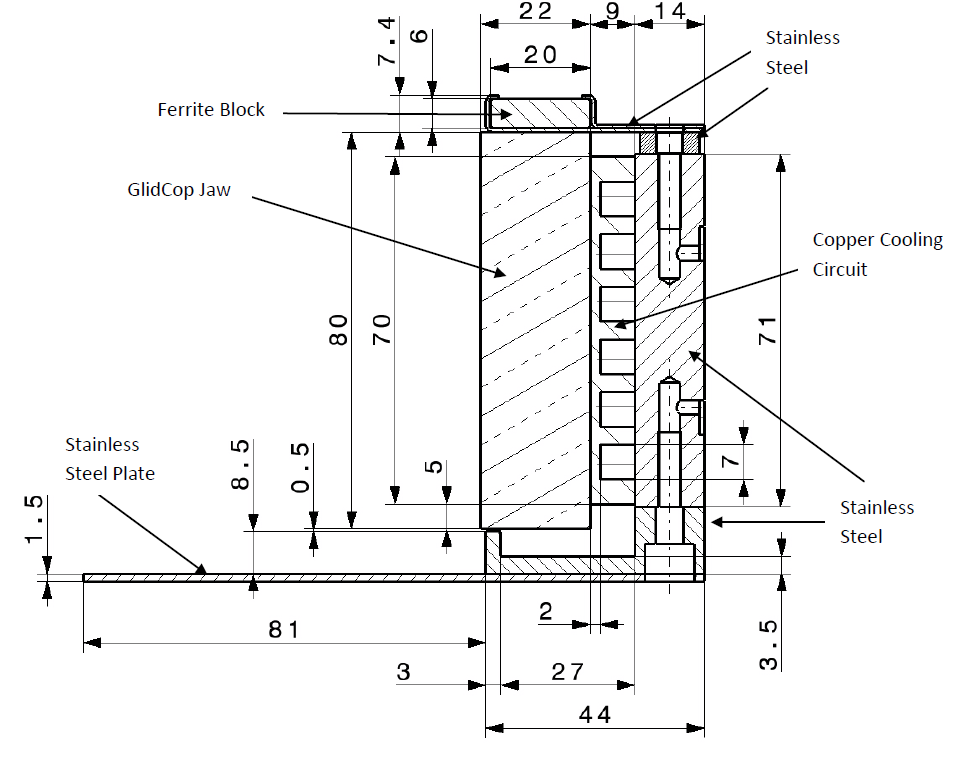
\includegraphics[width=0.7\textwidth]{LHC_Collimation_Upgrades/figures/cu-geo.png}
\end{center}
\label{fig:phase-2-rf-system}
\caption{The RF system for use in the phase 2 collimation system. The sliding RF contacts of the phase 1 design are replaced with a ferrite damping system. The RF contacts are removed, allowing the beam to see the entire RF cavity, causing resonances at lower frequencies. The Q of these resonances are decreased by the use of ferrite damping tiles.}
\end{figure}

In this chapter shall be presented an comparison of the different jaw materials proposed for use in the phase 2 secondary collimators, in particular a combination of jaw materials aimed at combining extremely robust materials with highly conductive metals, and the results of full 3D simulations of a TCTP collimator - a tertiary collimator for use in the LHC - which is incorporates the ferrite damping system in comparison to the sliding contacts of the phase 1 RF system. 



%
% Introduction to the new collimator design - Old collimator design, problems with sliding rails, new design, new material possibilities
% Material Evaluation - Comparison of CST simulations
% Whole collimator simulations of phase 2 secondary - Transverse and longitudinal modes with ferrite - compared to that from phase 1
% Sims in CST PS, GdFidl and HFSS
% Heating calculations also
%
%
%
%
%





%%%%% Wakefields and Impedances %%%%%%%

\chapter{Wakefields and Impedance}
\section{Wakefields}

Wakefields are the conventional name given to the phenomenon of induced electromagnetic fields due to charged particles traversing the beam pipe, RF cavities and many other pieces of equipment facing a particle beam in a particle accelerator. They have long been studied as a source of collective instabilities within particle accelerators [cite], through the use of analytical models for different beam pipe geometries[cite] and materials[cite], using computational simulation tools[cite], and both beam-based and bench-top measurement techniques. In this chapter is presented a number of significant properties of wakefields and their frequency domain counterpart, beam coupling impedance, as well an select example of observable effects that wakefields produce.

To aid in the explaination there will first be a short definition of the relative positions and labels of particles used in the following section. We define the source, or inducing particle as a charged particle with charge $q_{1}$ moving with velocity $\mathbf{v} = \beta{}c \mathbf{\vec{z}}$ at coordinate $\left( \mathbf{r_{1}} \right) = x_{1}\mathbf{\hat{x}} + y_{1}\mathbf{\hat{y}} + z_{1} \mathbf{\hat{z}}$, leading a test, or witness particle, with charge $q_{2}$, moving with velocity $\mathbf{v}$ at coordinate $\left( \mathbf{r_{2}} \right) = x_{2}\mathbf{\hat{x}} + y_{2}\mathbf{\hat{y}} + z_{2} \mathbf{\hat{z}}$ at a distance $z_{1} - z_{2}$ behind the source particle. This relationship is visualised in Fig.~\ref{fig:source_and_wit}.

\begin{figure}

\caption{The relative displacements and velocities of the source and test particles.}
\label{fig:source_and_wit}
\end{figure} 

\subsection{The Electromagnetic Fields of a Moving Charged Particle in Free Space}

If we consider the electromagnetic fields generated by the source particle, it can be shown that the fields at a vector $\mathbf{R} = \mathbf{r_{1}} - \mathbf{r_{2}}$ is given by

\begin{align}
\mathbf{E}\left( \mathbf{R}  \right) = \frac{q_{1}\mathbf{R}}{\gamma^{2}\left| \mathbf{R} \right|^{3}} \\
\mathbf{H}\left( \mathbf{R}  \right) = \frac{1}{c}\mathbf{v} \times \mathbf{E}
\label{eqn:gen_fields_mov_part}
\end{align}

where $\gamma = \sqrt{1- v^{2}/c^{2}}$ is the relativistic gamma factor. It can be shown that, if we take the ultrarelativistic limit (i.e. $\gamma \rightarrow \infty$) we can see that Eqn~\ref{eqn:gen_fields_mov_part} becomes

\begin{equation}
\mathbf{E}\left( \mathbf{R}  \right) = \frac{2q_{1}\mathbf{r}}{r^{3}}\delta{z-ct} \\
\mathbf{H}\left( \mathbf{R}  \right) = \mathbf{\hat{z}} \times \mathbf{E}
\label{eqn:ultrarel_field_eqn}
\end{equation}

where $\mathbf{r} = x\mathbf{\hat{x}} + y\mathbf{\hat{y}}$ is a purely transverse vector.

The following witness particle this experiences the resulting lorentz force 

\begin{equation}
\mathbf{F}\left(\mathbf{r_{1}}, \mathbf{r_{2}}  \right) = q_{2}\left[ \mathbf{E} + \mathbf{v} \times \mathbf{B}  \right]. 
\end{equation}

Looking at Eqn.~\ref{eqn:ultrarel_field_eqn}, it can be seen that the force can be seperated into longitudinal and transverse components 

\begin{align}
F_{\parallel}\left(\mathbf{r_{1}} \mathbf{r_{2}}  \right) = q_{2}E_{\parallel} \\
\mathbf{F_{\perp}}\left(\mathbf{r_{1}}, \mathbf{r_{2}}  \right)  = q_{2}\left[ \mathbf{E_{\perp}} + \mathbf{v} \times \mathbf{B} \right]
\end{align}

where $E_{\parallel} = \mathbf{E}.\mathbf{\hat{z}}$ and $\mathbf{E_{\perp}} = E_{x}\mathbf{\hat{x}} + E_{y}\mathbf{\hat{y}}$. $F_{\parallel}$ has only an electric component as the magnetic flux density $\mathbf{B}$ has magnitude = 0 in the $\mathbf{\hat{z}}$ direction. Considering just the longitudinal force, integrating over all space gives the total energy change of the source particle

\begin{equation}
U_{1}\left(\mathbf{r_{1}}  \right) = -q_{2} \int^{\infty}_{-\infty} d\mathbf{z} . \mathbf{F}\left(\mathbf{r_{1}}, \mathbf{r_{2}}  \right),
\end{equation}

where $t = z_{1}/\beta{}c = z_{1}/c$ in the ultrarelativistic case. Similarly the energy change in the witness particle can be calculated by

\begin{equation}
U_{2}\left(\mathbf{r_{1}}, \mathbf{r_{2}}, \tau  \right)  = -q_{2} \int^{\infty}_{-\infty} d\mathbf{z} \mathbf{F}\left(\mathbf{r_{1}}, \mathbf{r_{2}}  \right),
\label{eqn:witness_energy_change_single}
\end{equation}

where $t = z_{1}/\beta{}c = z_{1}/c + \tau$ and $\tau = \left( z_{1}-z_{2} \right)/\beta{}c$ is the time between the source and witness particle. From these two energy losses two widely used terms can be extracted; the loss factor $k$, given by

\begin{equation}
k\left(\mathbf{r_{1}}  \right) = \frac{U_{1}\left(\mathbf{r_{1}}  \right)}{q_{1}}
\end{equation}

and the longitudinal wake function, given by

\begin{equation}
w_{\parallel}\left(\mathbf{r_{1}}, \mathbf{r_{2}}, \tau   \right) = \frac{U_{2}\left(\mathbf{r_{1}}, \mathbf{r_{2}}, \tau  \right) }{q_{1} q_{2}},
\label{eqn:long_wake_func}
\end{equation}

denoting the normalised (with respect to source charge, and source and witness charge respectively) energy change of both the source particle (loss factor) and witness particle (wake function). 

\subsection{Wakefields of a Bunch}

As colliders are often used to collide bunches of particles as opposed to single particles, it is useful to be able to define the wake function of a bunch distribution. It can be seen that the total source charge of a bunch $q_{1}$ is the integral of the longitudinal current distribution $i_{b}\left( \tau \right)$ integrated over all time

\begin{equation}
q_{1} = \int^{\infty}_{-\infty}i_{b}\left( \tau \right) d\tau{}.
\end{equation}

The wake function of a bunch distribution at a point at time $\tau$ can be calculated by the convolution of the single particle wake function with the bunch distribution. Thus, if the bunch is split into infinitesimally small slices, the change in energy of a witness particle of charge $q$ at time $\tau$ due to a slice at time $\tau{}'$ is given by

\begin{equation}
dU\left(\mathbf{r_{2}}, \tau-\tau{}'  \right) = q i_{b}\left( \tau{}' \right) w_{\parallel}\left( r_{2}, \tau{}-\tau{}' \right).
\end{equation}

The longitudinal bunch wake function $W_{\parallel}\left(\mathbf{r_{2}}\right)$ can then be calculated using Eqn.~\ref{eqn:witness_energy_change_single}

\begin{equation}
W_{\parallel}\left( \mathbf{r_{2}}, \tau \right) = \frac{U\left( r_{2}, \tau \right) }{q_{1} q_{2}} = \frac{1}{q_{1}}\int^{\infty}_{-\infty}i_{b}\left( \tau{}' \right) w_{\parallel}\left( r_{2}, \tau{}-\tau{}'\right) d\tau{}' .
\end{equation}

\subsection{Transverse Wakefields}

Similar to the longitudinal wakefield, we can see that the total tranverse momentum change of the witness particle is given by integrating the transverse force across all space

\begin{equation}
\mathbf{P}\left(\mathbf{r_{1}}, \mathbf{r_{2}}, \tau  \right) = \int^{\infty}_{-\infty} \mathbf{F_{\perp}} \left( \mathbf{r_{1}} \mathbf{r_{2}}\right) dz
\end{equation}

where $t = z_{1}/c + \tau$ and again $\tau$ is the time delay between source and witness particles. And similarly to the longitudinal plane we can define a wake function normalised with regards to the source and witness particle charges

\begin{equation}
\mathbf{w_{\perp}}\left(\mathbf{r_{1}}, \mathbf{r_{2}}, \tau  \right) = \frac{\mathbf{P}\left(\mathbf{r_{1}}, \mathbf{r_{2}}, \tau  \right)}{q_{1} q_{2}}.
\label{eqn:trans_wake_func}
\end{equation}

And in a similar manner to the longitudinal bunch wake function a form for the transverse bunch wake function can be derived

\begin{equation}
W_{\perp}\left( \mathbf{r_{2}}, \tau \right) = \frac{U\left( r_{2}, \tau \right) }{q_{1} q_{2}} = \frac{1}{q_{1}}\int^{\infty}_{-\infty}i_{b}\left( \tau{}' \right) w_{\perp}\left( r_{2}, \tau{}-\tau{}'\right) d\tau{}' .
\end{equation}

\subsection{Panowsky-Wenzel Theorem}

Considering the force acting on the witness particle it can be seen to simply by the Lorentz force

\begin{equation}
\mathbf{F} = q_{2} \left[\mathbf{E} + \mathbf{v}\times \mathbf{B} \right]
\label{eqn:wit_gen_force}
\end{equation}

Now, considering Faraday's law in integral form ($\mathbf{B} = -\int^{t_{2}}_{t_{1}} \left( \nabla \times \mathbf{E} \right) dt$, $t_{1}$ being sufficiently in the past that $\nabla \times \mathbf{E} \rightarrow 0$), Eqn.~\ref{eqn:wit_gen_force} can be rewritten as

\begin{equation}
\mathbf{F} = q_{2}  \left[\mathbf{E} - \mathbf{v}\times\left(  \int^{t_{2}}_{t_{1}} \nabla \times \mathbf{E} dt \right) \right].
\end{equation}

Now, using the fact that the velocity $\mathbf{v}$ is constant and some vector identities this then becomes

\begin{equation}
\mathbf{F} = q_{2}  \left[\mathbf{E} - \int^{t_{2}}_{t_{1}}\left(  \nabla \left( \mathbf{v} . \mathbf{E} \right)  - \mathbf{v}\left( \nabla . \mathbf{E} \right) \right) dt  \right].
\end{equation}

If this force is seperated into the longitudinal and transverse components we see that they are the following

\begin{align}
F_{\parallel} = q_{2} E_{z} \\
\mathbf{F}_{\perp} = q_{2}  \left[\mathbf{E_{\perp}} - v \int^{t_{2}}_{t_{1}}\left(  \nabla_{\perp}E_{z}  - \frac{\partial\mathbf{E}_{\perp}}{\partial z} \right) dt  \right]
\end{align}

where $\nabla_{\perp}$ in the differential operator only in the transverse coordinates. If these are now compared to the identities of the wake function for the longitudinal and transverse wake functions given in Eqns.~\ref{eqn:long_wake_func; eqn:trans_wake_func} respectively, it can be seen that

\begin{align}
w_{\parallel}\left( \mathbf{r_{1}}, \mathbf{r_{2}}, \tau   \right) = -\frac{1}{q_{1}} \int^{\infty}_{-\infty} dz E_{z} \left( \mathbf{r_{1}}, \mathbf{r_{2}} \right) \\
\mathbf{w}_{\perp} \left(\mathbf{r_{1}}, \mathbf{r_{2}}, \tau   \right) = \frac{1}{q_{1}} \int^{\infty}_{-\infty} dz \left[ \mathbf{E_{\perp}}\left(\mathbf{r_{1}}, \mathbf{r_{2}} \right) - v   \int^{t_{2}}_{t_{1}}\left(  \nabla_{\perp}E_{z}\left(\mathbf{r_{1}}, \mathbf{r_{2}} \right)  - \frac{\partial\mathbf{E}_{\perp}\left(\mathbf{r_{1}}, \mathbf{r_{2}} \right)}{\partial z} \right) dt \right] \label{eqn:trans_wake_middle}.
\end{align}

The next stage requires partially differentiating Eqn~\ref{eqn:trans_wake_middle} by $s = v \tau = vt - z$. It can be seen from this relationship that $\partial / \partial s = - \partial / \partial z$ and $\partial / \partial s = 1/v \partial / \partial z$. Thus the first term can be replaced by $\partial / \partial s = - \partial / \partial s$, and the term the integral becomes the value of the intergrand at $\tau$.

\begin{equation}
\frac{\partial}{\partial s}\mathbf{w}_{\perp} \left(\mathbf{r_{1}}, \mathbf{r_{2}}, \tau   \right) = \frac{1}{q_{1}} \int^{\infty}_{-\infty} dz \left[ \frac{-\partial}{\partial z}\mathbf{E_{\perp}} - \left(  \nabla_{\perp}E_{z} + \frac{\partial\mathbf{E}_{\perp}}{\partial z} \right) dt \right].
\end{equation} 

It can be seen that the first and third integrand cancel. Also, the operator $\nabla_{\perp}$ may be moved to the front of the operation without changing the equation, thus

\begin{equation}
\frac{\partial}{\partial s}\mathbf{w}_{\perp} \left(\mathbf{r_{1}}, \mathbf{r_{2}}, \tau   \right) =  \frac{1}{q_{1}} \int^{\infty}_{-\infty} dz \nabla_{\perp}E_{z} = \mathbf{\nabla_{\perp}} w_{\parallel}\left( \mathbf{r_{1}}, \mathbf{r_{2}}, \tau   \right).
\end{equation}

%\begin{itemize}
%\item{Introduction to the electromagnetic field of charged particle moving in free space}
%\item{Field of a particle in a perfectly conducting pipe - method of image currents}
%\item{Place a witness particle distance s behind source particle and deduce electric field as seen by this particle}
%\item{normalise this by the source particle charge to give the wakepotential}
%\item{And again by the source particle charge and current profile to acquire the loss factor}
%\item{Longitudinal field predominantly}
%\item{Introduce the Panowsky-Wenzel theorem covering transverse field - Transverse wakes}
%\end{itemize}

\section{Impedances}

In a particle accelerator there are a large number of components that have frequency dependent properties, either due to their geometry (for example resonant cavity structures) or material properties (frequency dependent permetivitty/permeability is devices, for example ferrite in normal conducting kicker magnets). In addition many instability mechanisms are strongly modal in nature, thus a frequency analysis of the possible sources of impedance is incredibly valuable. 

\subsection{Beam Coupling Impedance}

The longitudinal beam coupling impedance $Z_{\parallel}$ and the transverse beam coupling impedance $Z_{\perp}$ are defined as the fourier transforms of the single particle wake function, given by

\begin{align}
Z_{\parallel} \left(\mathbf{r_{1}}, \mathbf{r_{2}}, \omega  \right) = \int^{\infty}_{0} d\tau w_{\parallel} \left(\mathbf{r_{1}}, \mathbf{r_{2}}, \tau  \right) e^{-j\omega \tau}\\
Z_{\perp} \left(\mathbf{r_{1}}, \mathbf{r_{2}}, \omega  \right) = j \int^{\infty}_{0} d\tau w_{\perp} \left(\mathbf{r_{1}}, \mathbf{r_{2}}, \tau  \right) e^{-j\omega \tau} \label{eqn:total_trans_imp}
\end{align}

where $\omega = 2\pi / \tau$. In a similar way the bunch wake function can be related to the longitudinal and transverse beam coupling impedance by considering the fourier transform of the time dependent bunch current $\lambda \left( \omega  \right) = \int^{\infty}_{-\infty} d\tau i_{b}\left( \tau \right) e^{-j \omega \tau}$, which allows it to be shown that

\begin{align}
W_{\parallel}  \left( \mathbf{r_{2}}, \tau \right) = \int^{\infty}_{- \infty} d \omega Z_{\parallel} \left(\mathbf{r_{1}}, \mathbf{r_{2}}, \omega  \right) \lambda \left( \omega  \right) e^{-j \omega \tau} \\
W_{\perp}  \left( \mathbf{r_{2}}, \tau \right) = \int^{\infty}_{- \infty} d \omega Z_{\perp} \left(\mathbf{r_{1}}, \mathbf{r_{2}}, \omega  \right) \lambda \left( \omega  \right) e^{-j \omega \tau}.
\end{align}

\subsection{Transverse Impedances}

As can be seen in Eqn.~\ref{eqn:total_trans_imp}, the transverse impedance is dependent on the displacement of both the source and witness particles. For reasons of simplifying beam dynamics evaluation, it is useful to distinguish the components dependent only on the transverse displacement of the source particle and that of the witness particle in the vertical and horizontal planes of the beam. This involves seperating the impedance firstly into horizontal and vertical components, and subsequently into components dependent only on the displacement of the source and of the witness particle. These are called the dipolar, or driving impedance and the quadrupolar, or detuning impedance respectively. In addition it can be shown that constant transverse terms exist which must also be taken into account. These are given by

\begin{align}
Z_{\perp} \left(\mathbf{r_{1}}, \mathbf{r_{2}}, \omega  \right)  &= Z_{\perp, x} \left( x_{1}, x_{2}, \omega \right) + Z_{\perp, y} \left( y_{1}, y_{2}, \omega \right) \\
Z_{\perp, x} \left( x_{1}, x_{2}, \omega \right) &= Z_{dip, x} \left( x_{1}, \omega  \right) + Z_{quad, x} \left( x_{2}, \omega  \right) + Z_{const, x} \left( \omega  \right) \\
Z_{\perp, y} \left( y_{1}, y_{2}, \omega \right) &= Z_{dip, y} \left( y_{1}, \omega  \right) + Z_{quad, y} \left( y_{2}, \omega  \right) + Z_{const, y} \left( \omega  \right).
\end{align}

The relative displacements of the source and witness particle are shown in Fig.~\ref{fig:trans_imp_disp} for clarity.

\begin{figure}

\caption{The relative displacements of the source and witness particle in the horizontal and vertical planes that identify the dipolar/driving and quadrupolar/detuning impedances.}
\label{fig:trans_imp_disp}
\end{figure}

%\begin{itemize}
%\item{Firstly mention the commonality of frequency dependent material properties - ferrite permeability, permitivitty determined by conductivity/frequency in conductors/dielectrics/skin depth}
%\item{Fourier transform of wakefield into the convolution of the beam current spectrum and the impedance}
%\item{Again Panowsky-Wenzel for impedance}
%\item{Discussion of the transverse impedance - in particular the general definition of an impedance (n-th order current interacting with an m-th order field)}
%\item{Define dipolar/driving and quadrupolar/detuning impedance. In addition constant transverse impedance term}
%\end{itemize}
\subsection{Geometric Impedance}
\label{sec:imp_geo_imp}

Geometric impedances are characterised by resonant fields at a resonant frequency, typically characterised by some characteristic dimension of the structure. This is typically a characteristic length of a structure (cavity size, antenna length), which may be part of a vacuum tank, or an internal structure to the device exhibiting the resonance. 

As a simple example, consider a cylindrical pillbox cavity of radius $r_{cav}$ and length $L$ connected to a beam pipe of radius $r_{pipe}$ located at the centre of the cavity, as shown in Fig.~\ref{fig:cylin_geo_diagram}. For simplicity we shall assume that the cavity is made from a perfectly conducting materials. It shall be assumed that the fields do not propogate along the attached beam pipe (i.e. for frequencies below cutoff). In this example we shall consider a particle travelling on the axis of the beam pipe, and only the longitudinal wakefunction/impedance will be investigated to simplify matters. Further details can be found in [cite Andy Wolzski, E Jensen, Stupakov]. It can be shown that there are two families of resonant modes in in a pillbox cavity, TM-type modes and TE-type modes. The TE-type modes have no longitudinal electrical field by definition, and therefore do not contribute to the longitudinal wakefunction for an on axis particle. In a cylindrical coordinate system using coordinates $(r, \theta, z)$, the longitudinal electrical field of the $n$-th order TM-type modes can be shown to be

\begin{equation}
E_{z,n} = E_{0}J_{n}\left( k_{r} r \right) cos \left( n \theta \right) cos \left( k_{z} z \right) e^{-j \omega t}
\end{equation}

where $E_{0}$ is the magnitude of the electric field, $J_{n}$ is $n$-th order Bessel function, $k_{z}=n\pi{}/L$, and n is an interger. A wakefunction for each mode subsequently be defined as $w_{\parallel ,n}\left( \tau \right)$, where the total wakefunction is thus defined as

\begin{equation}
w_{\parallel} \left( \mathbf{r}_{1}, \mathbf{r}_{2}, \tau \right) =  \displaystyle\sum\limits_{n = 0}^{\infty} w_{\parallel ,n} \left( \tau \right) = \displaystyle\sum\limits_{n = 0}^{\infty} \int^{\infty}_{-\infty} dz E_{z,n} \left( r, \theta , z \right)
\end{equation}

\begin{figure}

\caption{Cross section of a cylindrical pillbox cavity with an attached beam pipe}
\label{fig:cylin_geo_diagram}
\end{figure}

To evaluate the problem in the frequency domain we shall introduce the RLC parallel circuit model to simplif the frequency doman representation.

\subsubsection{RLC Circuit Model}

We can define any given resonance by an equivalent RLC circuit, which is driven by a current, shown in Fig.~\ref{fig:rlc_circ}. The symbols represent the equivalent resistor (R), inductance (L) and capcitance (C). From this circuit a number of defining parameters are now deduced, and the physical equivalents in the physical cavity are described.

\begin{figure}

\caption{The equivalent RLC parallel circuit for a cavity resonance, driven by a current $i_{b}$, in this cas the beam current}
\label{fig:rlc_circ}
\end{figure}

The first parameter to be derived is the resonant frequency of the cavity mode itself $\omega_{0}$. This can be shown (by solving the time varying voltage build up of the circuit in Fig.~\ref{fig:rlc_circ}) to be given by

\begin{equation}
\omega_{0} = \frac{1}{LC}.
\end{equation}

Next we define the quality factor of the cavity mode, $Q_{n}$. This factor describes the damping of the wakefunction in the cavity for a given mode, larger values indicating a longer damping time. In terms of the cavity it is given by

\begin{equation}
Q_{n} = \frac{\omega_{0} W}{P_{loss}} = \omega_{0}RC
\end{equation}

where $W = \int_{V} \epsilon / 2 \left| \mathbf{E} \right|^{2} dV$ is the stored electromagnetic energy in the cavity due to the mode, and $P_{loss}$ is the total losses in the cavity. Commonly the later is dominated by conductive losses on the cavity walls, but as will be seen in later sections, also includes losses due to other mechanisms. The final figures of merit are the $R_{s, n}/Q_{n}$ of the cavity mode, and the shunt impedance $R_{s, n}$ of the mode. $R_{s, n}/Q_{n}$ is given by

\begin{equation}
\frac{R_{s, n}}{Q_{n}} = \frac{\left| V_{acc} \right|^{2}}{2 \omega_{0} W}
\end{equation}

where $V_{acc} = \int^{\infty}_{-\infty} E_{z, n} e^{-j \omega_{0} z/ \beta{}c} dz$ is the effective voltage that a traversing particle sees due to the cavity mode. It can thus be seen that the $R_{s, n}/Q_{n}$ of a cavity mode gives some ratio of the acceleration of a traversing particle to the stored energy. The shunt impedance $R_{s, n}$ is then given by

\begin{equation}
R_{s, n} = \left(  \frac{R_{s, n}}{Q){n}} \right) Q_{n} = \frac{\left| V_{acc} \right|^{2}}{2 P_{loss}}
\end{equation}

or an equivalent ratio for power loss in the cavity to acceleration of the particle. From these quality factors is defined a broadband description of the beam coupling impedance at all frequencies due to all modes, given by

\begin{equation}
Z_{\parallel} \left( \omega \right) = \displaystyle\sum\limits_{n = 0}^{\infty} Z_{\parallel, n} \left( \omega \right) = \displaystyle\sum\limits_{n = 0}^{\infty} \frac{R_{s, n}}{1 - iQ \left( \frac{\omega}{\omega_{0}} - \frac{\omega_{0}}{\omega} \right)}.
\end{equation}

And number of examples of this type of impedance are shown in Sec.~\ref{sec:beam_induced_heating}
\subsection{Resistive Wall Impedance}
\label{sec:res_wall_imp}

The resistive wall impedance is an impedance generated due to the finite conductivity of the material of the beam pipe wall. This can have a number of regimes dependent on whether the skin depth of the material $\delta \left( \omega \right) = \sqrt{\frac{2}{\mu_{0} \sigma \omega}}$ is much smaller than the thickness of the beam pipe wall [ref classical thick wall formalism], comparable to the thickness of the beam pipe wall [ref redistribution effect] or much larger than the thickness of the beam pipe wall [ref dielectric or ferrite impedances]. In this instance, $\sigma$ is the conductivity of wall material. It can also be shown that the shape of the beam pipe cross section also plays a significant role in defining the impedance [ref mounet axisymmetric/parallel plate].

Here we shall not attempt a comprehensive summary of the various resistive wall impedance models, but simply give an introduction to the classic thick wall formalism to give a sense of how changing the wall conductivity affects the resistive wall impedance. A considerably more detailed overview of this derivation can be found in [cite Chao]. Consider a circular beam pipe of radius $a$ containing a source particle of charge $q_{1}$ moving with velocity $\mathbf{v} = \beta c \mathbf{\hat{z}}$, as shown in Fig.~\ref{fig:res_wall_diagram}. In this case it shall be assumed that $\beta = 1$.

\begin{figure}

\caption{The geometry of the classical thick wall formula.}
\label{fig:res_wall_diagram}
\end{figure}

It can be shown that the beam coupling impedance per unit length $L$ of this structure, assuming $\delta \ll b$ is given by [cite Chao]

\begin{align}
\frac{Z_{\parallel}^{0}  \left( \omega \right)}{L} &= \frac{1 - sgn \left( \omega \right) i }{2 \pi a \delta \sigma} \\
\frac{Z_{\perp}^{1}  \left( \omega \right)}{L} &= \frac{c}{\omega}\frac{1 - sgn \left( \omega \right) i }{2 \pi a^{3} \delta \sigma}
\end{align}

where $sgn$ is a function that returns the sign (positive or negative) of the value. The 0 and 1 indicate these modes represent the zeroeth and first azimuthal modes of the source current. It can be easily seen is that the impedance is proportional to $1/ \sqrt{\sigma}$, thereby indicating that materials with a higher conductivity generally give lower beam coupling impedance in the thick wall regime (See Fig.~\ref{fig:resWallImpComp} for a comparison between two sample materials).

\begin{figure}
\subfigure[]{

\label{fig:reswalllong}
}
\subfigure[]{

\label{fig:reswalltrans}
}

\caption{Examples of the longitudinal \ref{fig:reswalllong} and transverse \ref{fig:reswalltrans} resistive wall impedance of a beam pipe of radius $a = 2cm$ made of both copper ($\sigma = 1 \times 10^{7} S m^{-1}$) and graphite ($\sigma = 7 \times 10^{4} S m^{-1}$.}
\label{fig:resWallImpComp}
\end{figure}

\begin{itemize}
\item{Return to simple axisymmetric geometry concerning a finite conductivity of the wall}
\item{Derive in frequency domain - then have impedance. Give an example wakefield of a good conductor (copper), bad conductor (graphite), non-conductor (ferrite)}
\end{itemize}
\section{Example of the Effects of Wakefields}
\subsection{Beam Induced Heating}
\label{sec:beam_induced_heating}
\section{Defining and Deriving Power Loss in Circular Accelerators}
\label{sec:power_loss}

When a charged particle interacts with an impedance it losses energy to generate the resulting wakefield. This is called the parasitic loss, and is generally defined as[ref Chao/Ng]

\begin{equation}
\Delta E = -2\pi e^{2}N_{b}\int^{\infty}_{-\infty} d\omega \left| \lambda \left( \omega \right)  \right|^{2} Z_{\parallel} \left( \omega \right)
\end{equation}

where $\Delta E$ is the energy loss per pass per particle, $e$ is the charge per particle, $N_{b}$, $\omega$ the frequency, $\lambda$ the line density of the bunch and $Z_{\parallel}$ the longitudinal impedance of the object being traversed.
																
Due to the decay of the wakefields induced by this energy loss, this energy must eventually be lost to the device causing the impedance (valid below the cutoff frequency of the machine beam pipe). Therefore we can assume that the energy loss from the particles is absorbed by the surrounding structure. Summing over all particles in a bunch we can therefore obtain a sum of the energy loss;

\begin{equation}
\Delta E_{bunch} = 2\pi \left( eN_{b}   \right)^{2} \int^{\infty}_{-\infty} d\omega \left| \lambda \left( \omega \right)  \right|^{2} Z_{\parallel} \left( \omega \right)
\end{equation}

As often we must deal with machines storing multiple bunches, for these we simply multiply the energy loss per bunch by the number of stored bunches to acquire the total energy loss per passage;

\begin{equation}
\Delta E_{bunches} = 2\pi \left( eN_{b}   \right)^{2}n_{bunch} \int^{\infty}_{-\infty} d\omega \left| \lambda \left( \omega \right)  \right|^{2} Z_{\parallel} \left( \omega \right)
\end{equation}

where $n_{bunch}$ is the number of bunches in the machine. If we assume a revolution frequency $f_{rev}$ we thus get a power loss of;

\begin{align}
P_{loss}  = & \Delta E_{bunches} f_{rev}\nonumber \\  
 = & 2\pi f_{rev} \left( eN_{b}   \right)^{2}n_{bunch} \int^{\infty}_{-\infty} d\omega \left| \lambda \left( \omega \right)  \right|^{2} Z_{\parallel} \left( \omega \right) \nonumber  \\ 
 = & 2\pi f_{rev} \left( eN_{b}   \right)^{2}n_{bunch} \int^{\infty}_{-\infty} d\omega \left| \lambda \left( \omega \right)  \right|^{2} Z_{\parallel} \left( \omega \right) \nonumber \\
 = & 2\pi f_{rev} \left( eN_{b}   \right)^{2}n_{bunch} \int^{\infty}_{-\infty} d\omega \left| \lambda \left( \omega \right)  \right|^{2} \left( \Re{}e \left( Z_{\parallel} \left( \omega\right) + \Im{}m Z_{\parallel} \left( \omega\right) \right) \right).
\end{align}
 
As $\Re{}e\left(Z_{\parallel} \left( \omega\right)\right)$ is an even function and $\Im{}m\left(Z_{\parallel} \left( \omega\right)\right)$ is an odd function, we see that

\begin{equation}
P_{loss}   =  \omega_{rev} \left( eN_{b}   \right)^{2}n_{bunch} \int^{\infty}_{0} 2 d\omega \left| \lambda \left( \omega \right)  \right| ^{2}  \Re{}e \left( Z_{\parallel} \left( \omega\right)  \right).
\label{eqn:power_loss_omega}
\end{equation}

Next we make a change of the variable of integration $\omega = n_{bunch}\omega_{rev}$;

\begin{equation}
P_{loss}   =  \omega_{rev} \left( eN_{b}   \right)^{2}n_{bunch}^{2} \int^{\infty}_{0} 2 d\omega_{rev} \left| \lambda \left( \omega_{rev}n_{bunch} \right)  \right|^{2}  \Re{}e \left( Z_{\parallel} \left( \omega_{rev}n_{bunch}\right)  \right).
\end{equation}

We can subsequently change to a sum formalism to obtain

\begin{equation}
P_{loss} = \left( \omega_{rev}eN_{b}n_{bunch}  \right)^{2} \displaystyle\sum\limits_{p = 0}^{\infty} \left( 2 \left| \lambda \left(p \omega_{rev}n_{bunch} \right)  \right|^{2}  \Re{}e \left( Z_{\parallel} \left(p \omega_{rev}n_{bunch}\right) \right) \right) \label{ean:heating-gen}
\end{equation}

where $\omega_{0} = 2\pi f_{0}$, $f_{0} = \frac{1}{\tau_{b}}$ and $\tau_{b}$ is the bunch spacing.

\section{Longitudinal Beam Profiles}

As shown by the derivations in Section~\ref{sec:power_loss}, asides from the longitudinal impedance of the device under consideration the longitudinal profile of the circulating bunches also contributes to the power loss in the machine. In past works it has generally been assumed that bunches in accelerators have a Gaussian profile [ref Sacherer/Grudiev/Laclare](seen in Eqn.~\ref{eqn:gauss}, where $4\sigma_{z} = t_{b}$, $t_{b}$ is the bunch length) when approaching the analytical treatment of beam instabilities, both single-bunch and multi-bunch. Recent measurements of the power spectrum of particle beams, especially in the LHC [ref theo/phillipe] have shown characteristics that the Gaussian profile does not predict, for example the high frequency secondary peak as seen in Fig.~\ref{fig:measured_gauss}. To make more realistic predictions of heat loss due to beam impedance in the machine it is thus necessary to find bunch profiles which reproduce this behaviour.

\begin{equation}
\lambda \left( t \right) = e^{\frac{-t^{2}}{2\sigma^{2}}}
\label{eqn:gauss}
\end{equation}

\begin{figure}
\subfigure[]{
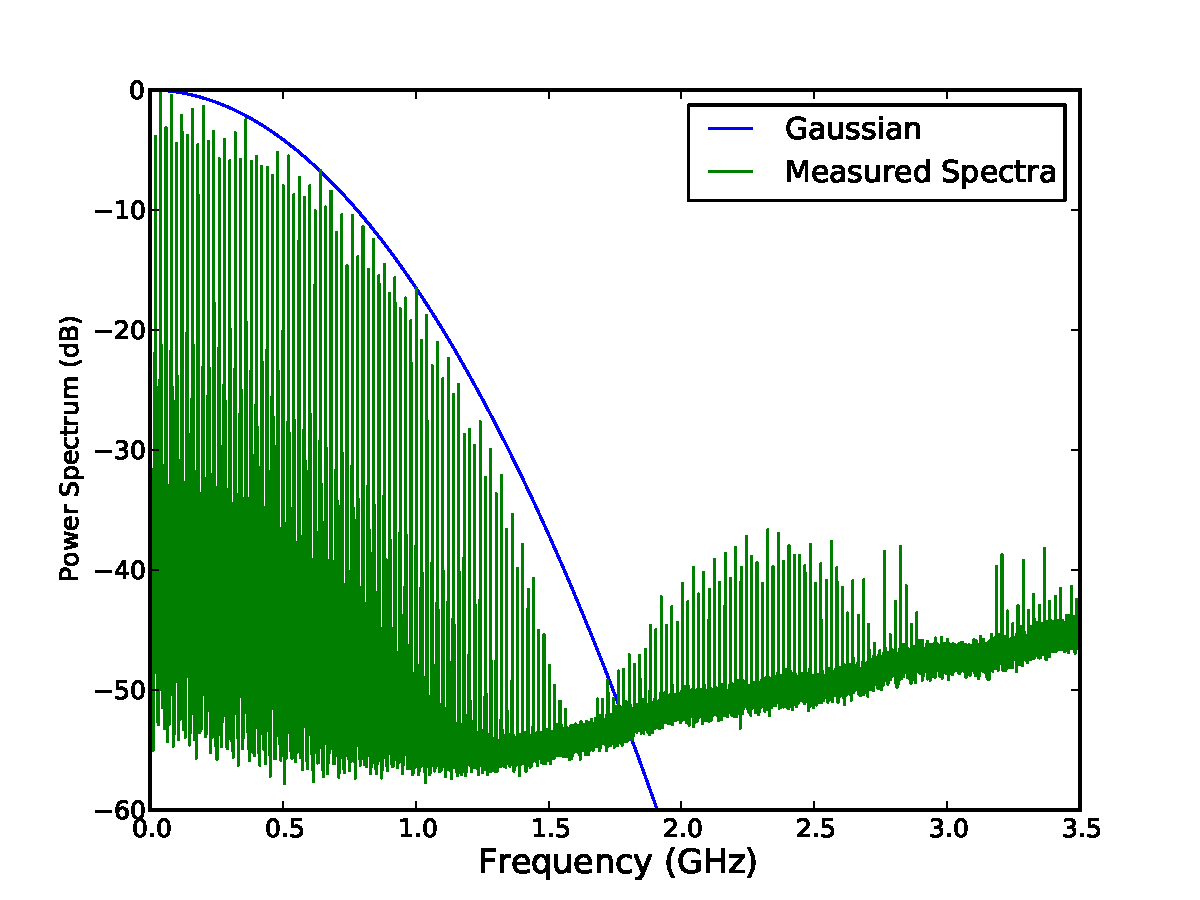
\includegraphics[width=0.45\textwidth]{Wakefields_and_Impedances/figures/beam_spectra_power_gauss_meas_12ns.pdf}
\label{fig:gauss_meas_freq}
}
\subfigure[]{
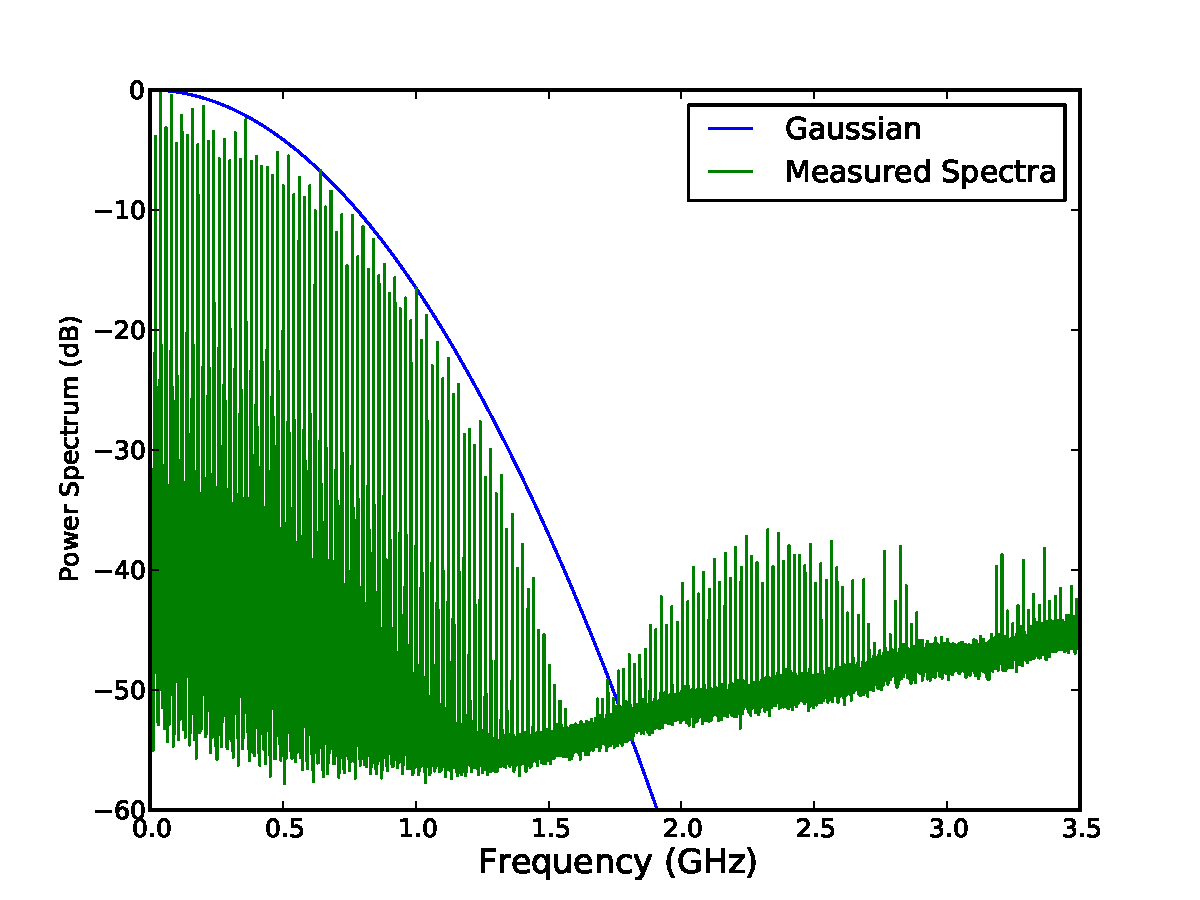
\includegraphics[width=0.45\textwidth]{Wakefields_and_Impedances/figures/beam_spectra_power_gauss_meas_12ns.pdf}
\label{fig:gauss_meas_time}
}
\caption{A comparison of \ref{fig:gauss_meas_freq} a measured beam power spectrum and a gaussian bunch of the same bunch length in the frequency domain and \ref{fig:gauss_meas_time} the resulting time domain beam profile. The gaussian has a bunch length (4$\sigma_{z}$ = 1.2ns) }
\label{fig:measured_gauss}
\end{figure}

A number of different longitudinal bunch profiles have been investigated in the past. Here we shall look at 3 other bunch profiles; a parabolic line density (see Eqn.~\ref{eqn:para_profile}), cos$^{2}$ (see Eqn.~\ref{eqn:cos_profile}), water-bag (see Eqn.~\ref{eqn:water_bag_profile}).

\begin{equation}
A\left( t \right) = \int^{\infty}_{-\infty} \lambda \left( \omega \right) e^{j\omega t} d\omega = 
\begin{cases}1-\left( \frac{2t} {t_{b}} \right)^{2} &\textrm{if $| t/2 | \leq t_{b}$}\\
0								&\textrm{if $| t/2 | > t_{b}$}
\end{cases}
\label{eqn:para_profile}
\end{equation}

\begin{equation}
A\left( t \right) = \int^{\infty}_{-\infty} \lambda \left( \omega \right) e^{j\omega t} d\omega = 
\begin{cases}
cos^{2}\left( \frac{\pi t} {t_{b}} \right) &\textrm{if $| t/2 | \leq t_{b}$}\\
0								&\textrm{if $| t/2 | > t_{b}$}
\end{cases}
\label{eqn:cos_profile}
\end{equation}

\begin{equation}
A\left( t \right) = \int^{\infty}_{-\infty} \lambda \left( \omega \right) e^{j\omega t} d\omega = 
\begin{cases}
\sqrt{1-\left( \frac{2t}{t_{b}}\right)^{2}} &\textrm{if $| t/2 | \leq t_{b}$}\\
0								&\textrm{if $| t/2 | > t_{b}$}
\end{cases}
\label{eqn:water_bag_profile}
\end{equation}

The comparison of these bunch profiles in the time domain are shown in Fig.~\ref{fig:time_bunch_profiles}. Note all bunch currents are normalised to their peak value. The corresponding current and power spectrums are shown in Fig.~\ref{fig:freq_dom_prof}. There are several things to note about these spectra; firstly that the non-infinite distribution of the non-gaussian bunch profiles gives rise to a number of high frequency lobes in the power spectrum, and secondly the interval of these nodes depends heavily on the bunch profile.

\begin{figure}
\begin{center}
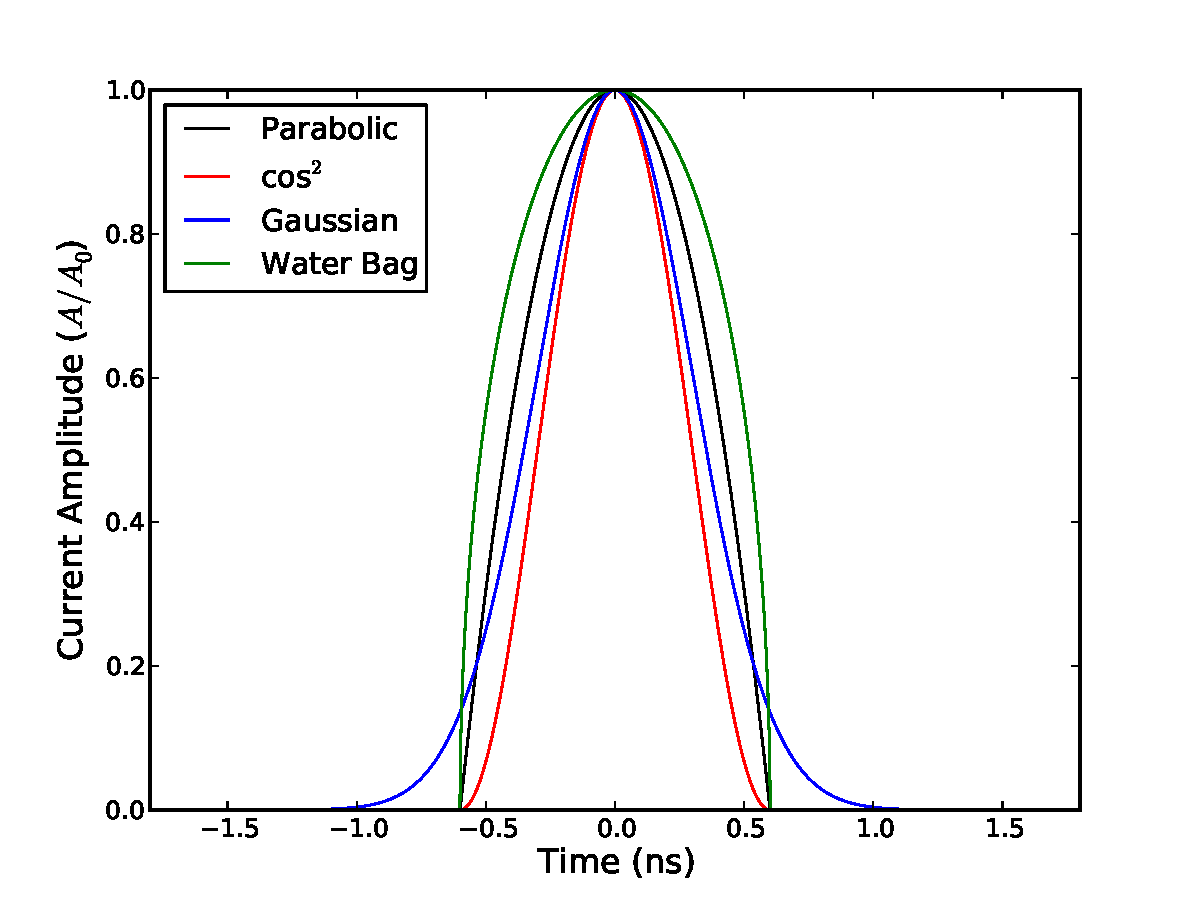
\includegraphics[width=0.65\textwidth]{Wakefields_and_Impedances/figures/bunch_profile_12ns.pdf}
\end{center}
\label{fig:time_bunch_profiles}
\caption{The longitudinal bunch profile of a number of bunch distributions. Note that all of them are normalised to have a peak bunch current of 1. For the gaussian distribution the bunch length is the 4$\sigma$ value. The bunch length $\tau_{b} = 1.2ns$}
\end{figure}

\begin{figure}
\subfigure[]{
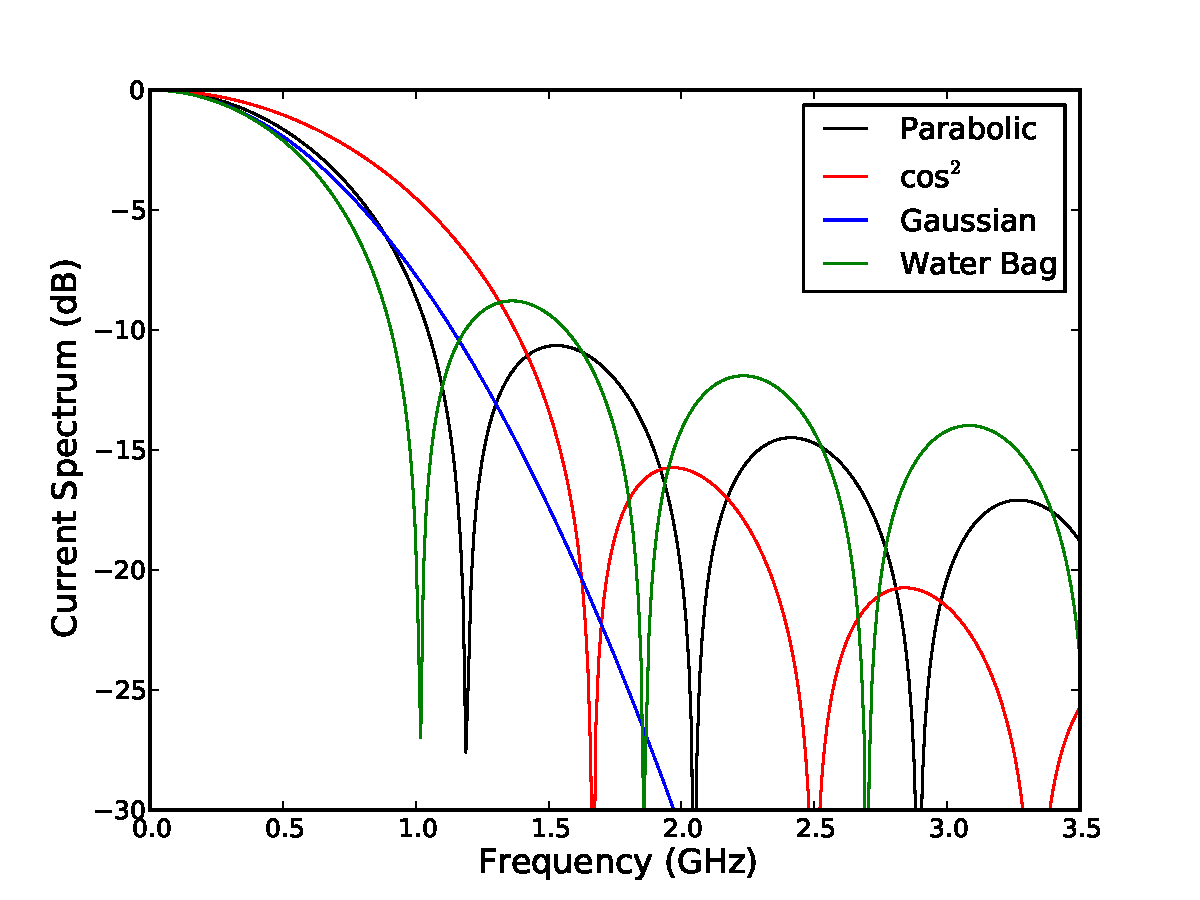
\includegraphics[width=0.45\textwidth]{Wakefields_and_Impedances/figures/current_spectrum_12ns.pdf}
\label{fig:current_spec}
}
\subfigure[]{
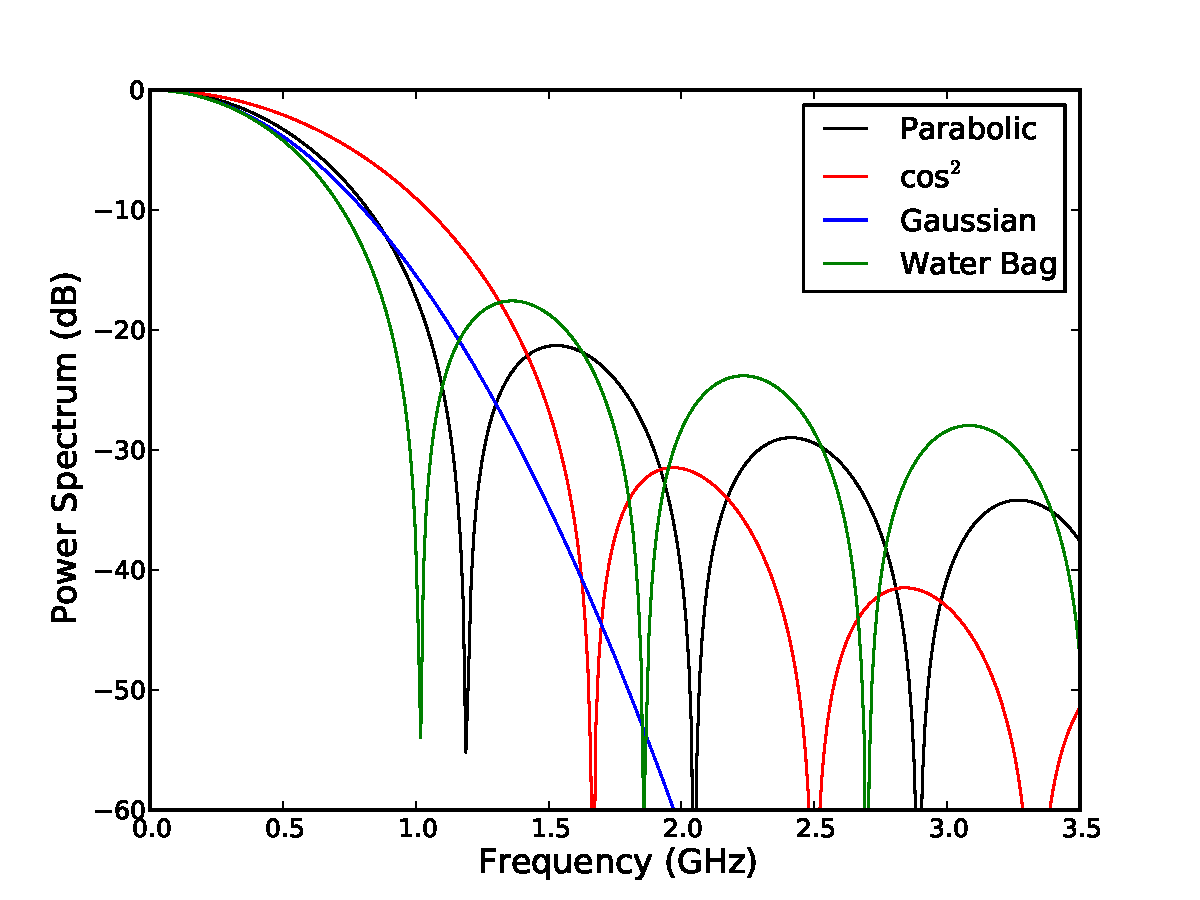
\includegraphics[width=0.45\textwidth]{Wakefields_and_Impedances/figures/power_spectrum_12ns.pdf}
\label{fig:power_spec}
}
\label{fig:freq_dom_prof}
\caption{The frequency domain \ref{fig:current_spec} current spectrum and \ref{fig:power_spec} power spectrum for a number of different bunch profiles with a bunch length $\tau_{b} = 1.2ns$.}
\end{figure}

To illustrate more clearly the effect of changing the bunch length on the power spectrum, a number of bunch profiles and the corresponding power spectra with different bunch lengths are shown below. Firstly, consider a gaussian bunch profile. It can be seen in Fig.~\ref{fig:diff_bunch_len_gauss} that by increasing the bunch length that the magnitude at high frequencies is decreased quite substantially as the bunch length increases. If we consider a finite bunch profile (non-gaussian), we note that we have high frequency lobes. The peak frequency of these lobes depends on the bunch length, as illustrated using a parabolic bunch profile for bunch lengths $\tau_{b} = 1ns, 1.2ns, 1.4ns$ in Fig.~\ref{fig:diff_bunch_len_para}. As the bunch length is increased the lobes move to lower frequencies, and the width of the first branch decreases, as seen for the gaussian bunch. Similar behaviour is observed with the cos$^{2}$ and water-bag bunch profiles.

\begin{figure}
\subfigure[]{
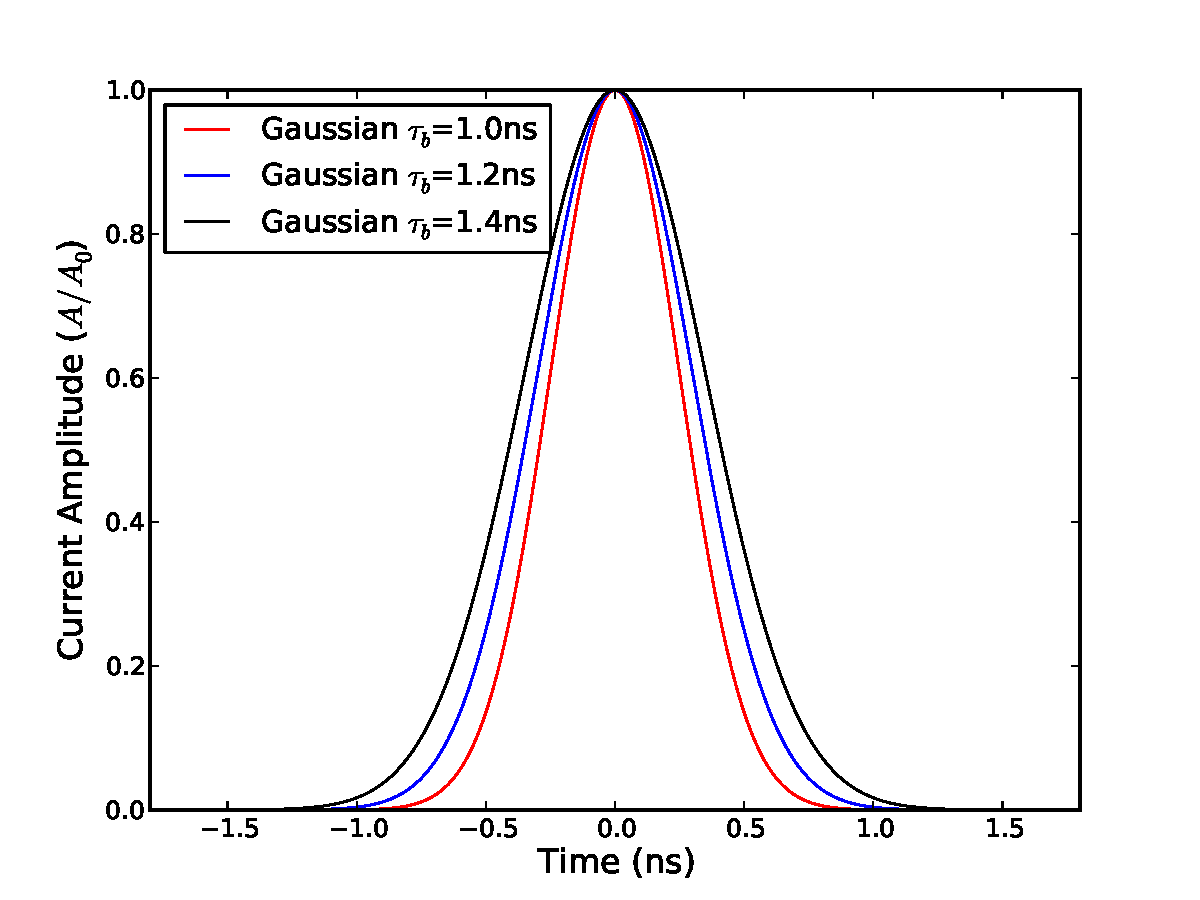
\includegraphics[width=0.45\textwidth]{Wakefields_and_Impedances/figures/gaussian_time_dom_diff_lengths.pdf}
\label{fig:change_len_time_gauss}
}
\subfigure[]{
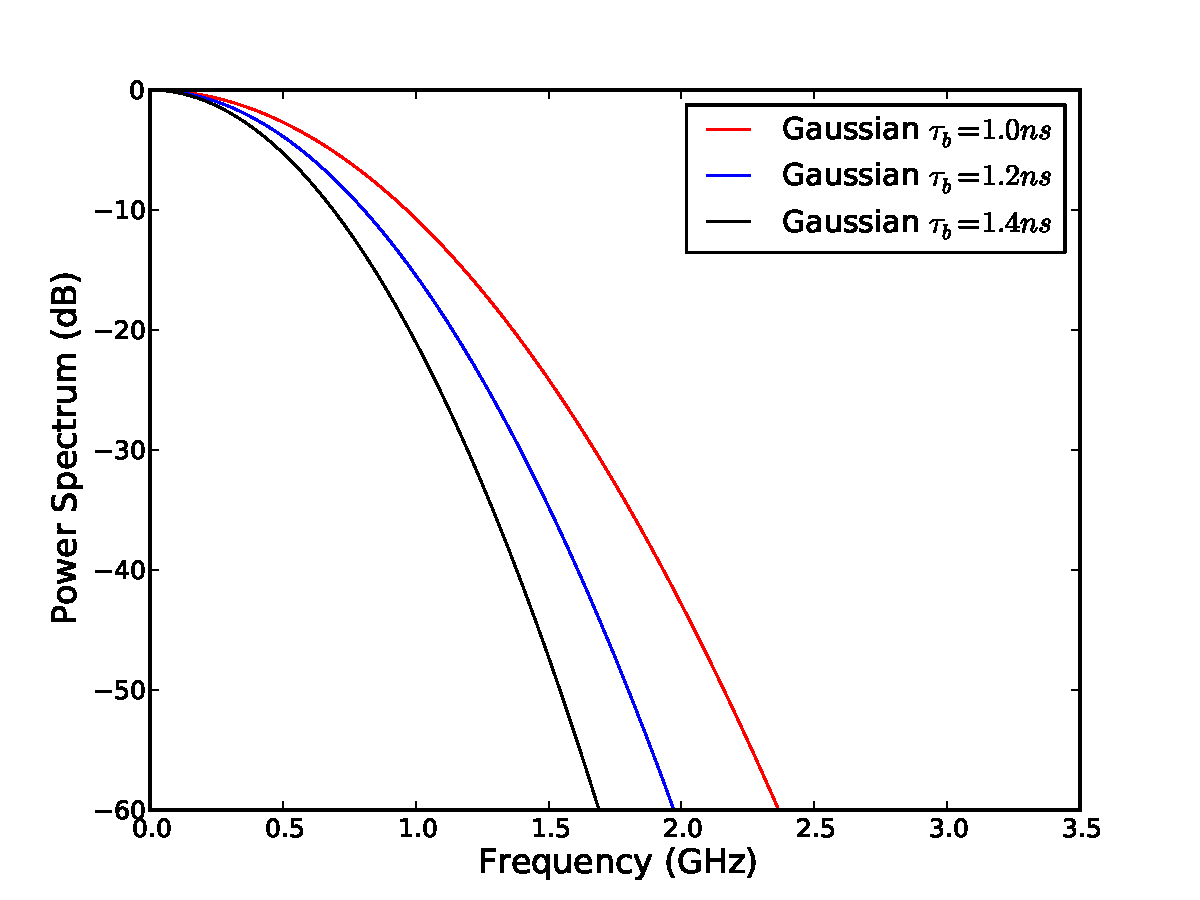
\includegraphics[width=0.45\textwidth]{Wakefields_and_Impedances/figures/gaussian_power_spec_diff_lengths.pdf}
\label{fig:change_len_freq_gauss}
}
\caption{\ref{fig:change_len_time_gauss} The longitudinal profile and the \ref{fig:change_len_freq_gauss} associated bunch power spectrum for a number of bunch lengths assuming a gaussian bunch profile.}
\label{fig:diff_bunch_len_gauss}
\end{figure}

\begin{figure}
\subfigure[]{
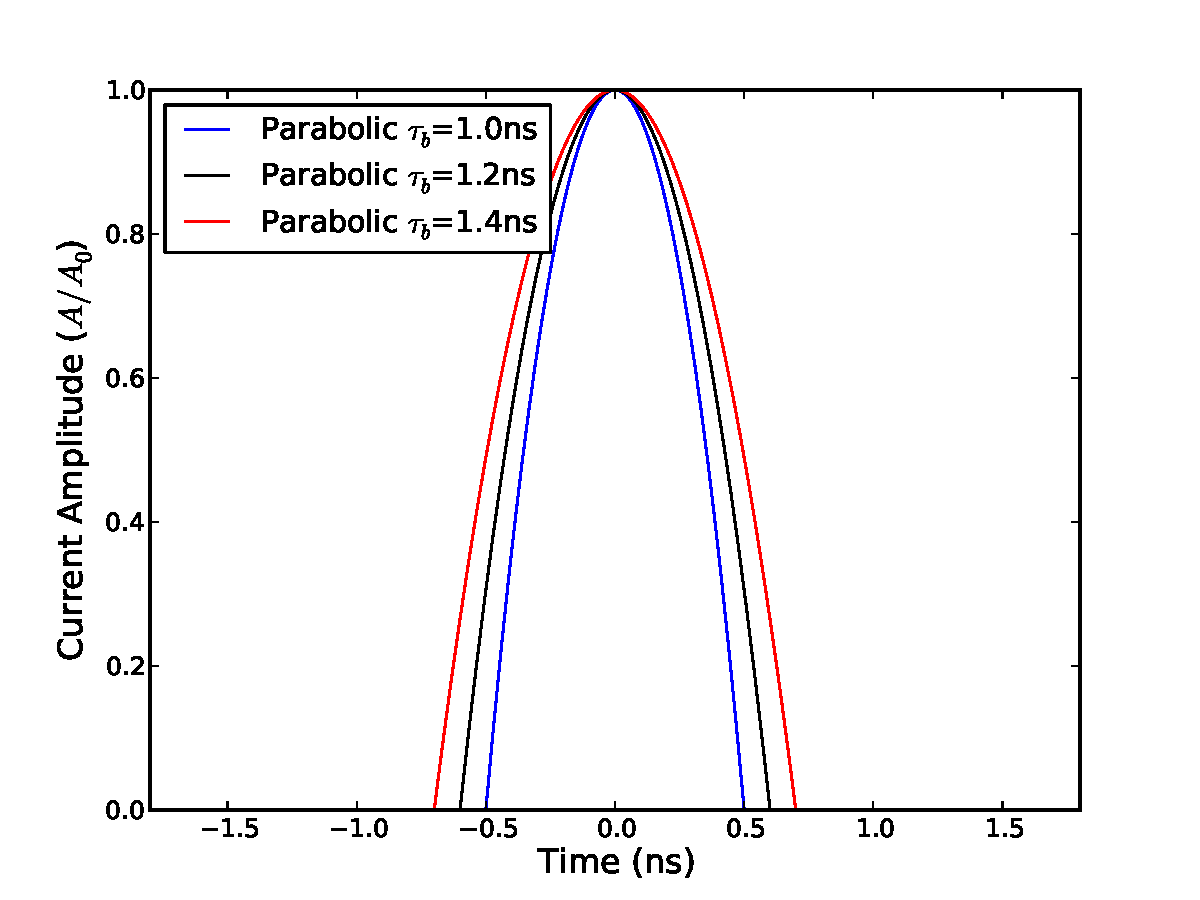
\includegraphics[width=0.45\textwidth]{Wakefields_and_Impedances/figures/current_amp_para_change.pdf}
\label{fig:change_len_time_para}
}
\subfigure[]{
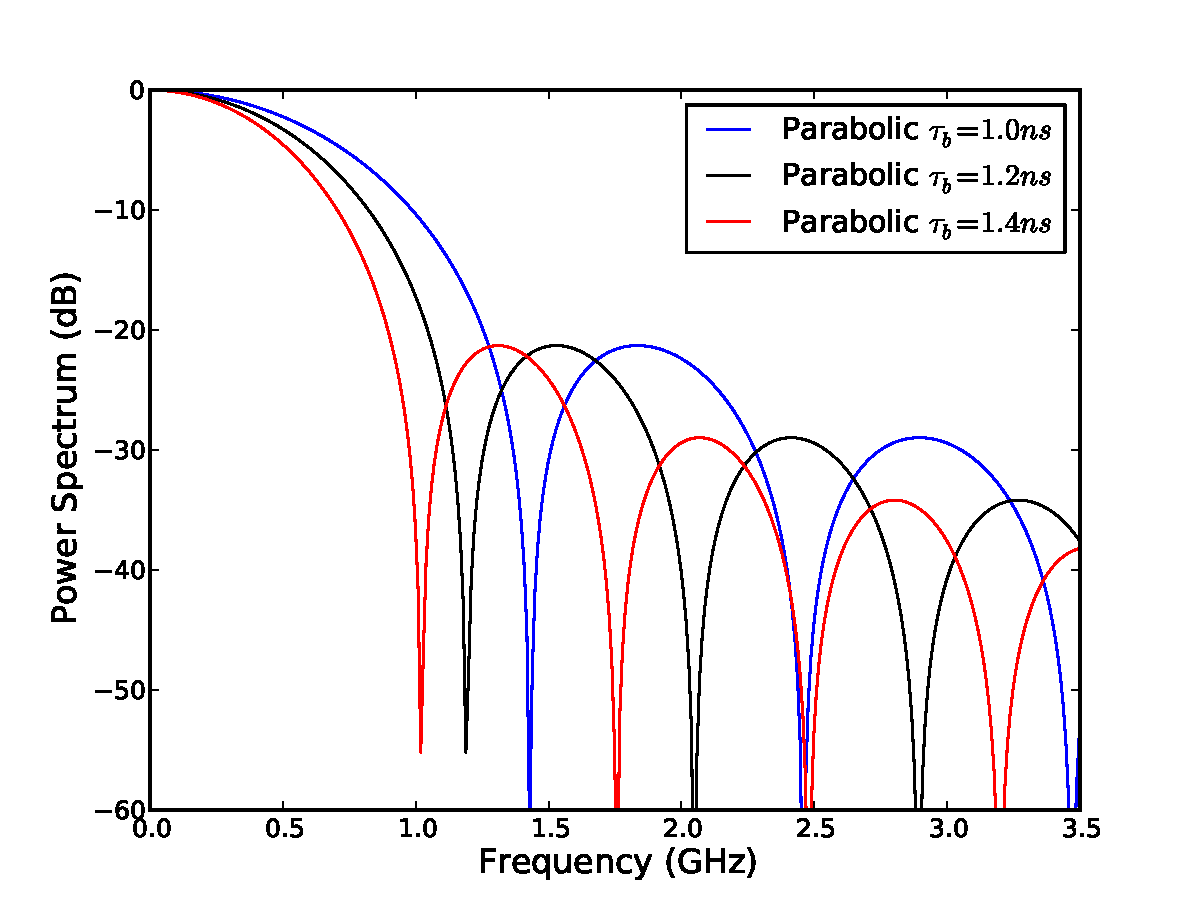
\includegraphics[width=0.45\textwidth]{Wakefields_and_Impedances/figures/freq_power_para_change.pdf}
\label{fig:change_len_freq_para}
}
\caption{\ref{fig:change_len_time_para} The longitudinal profile and the \ref{fig:change_len_freq_para} associated bunch power spectrum for a number of bunch lengths assuming a parabolic bunch profile.}
\label{fig:diff_bunch_len_para}
\end{figure}

Finally, a comparison of a measured bunch power spectra and the analytical power spectra is shown in Fig.~\ref{fig:power_all}. It can be seen that whilst it is possible to replicate some of the properties of the measured spectrum, an exact replication is non-trivial. Further investigation into the appropriate bunch profile is ongoing.

\begin{figure}
\begin{center}
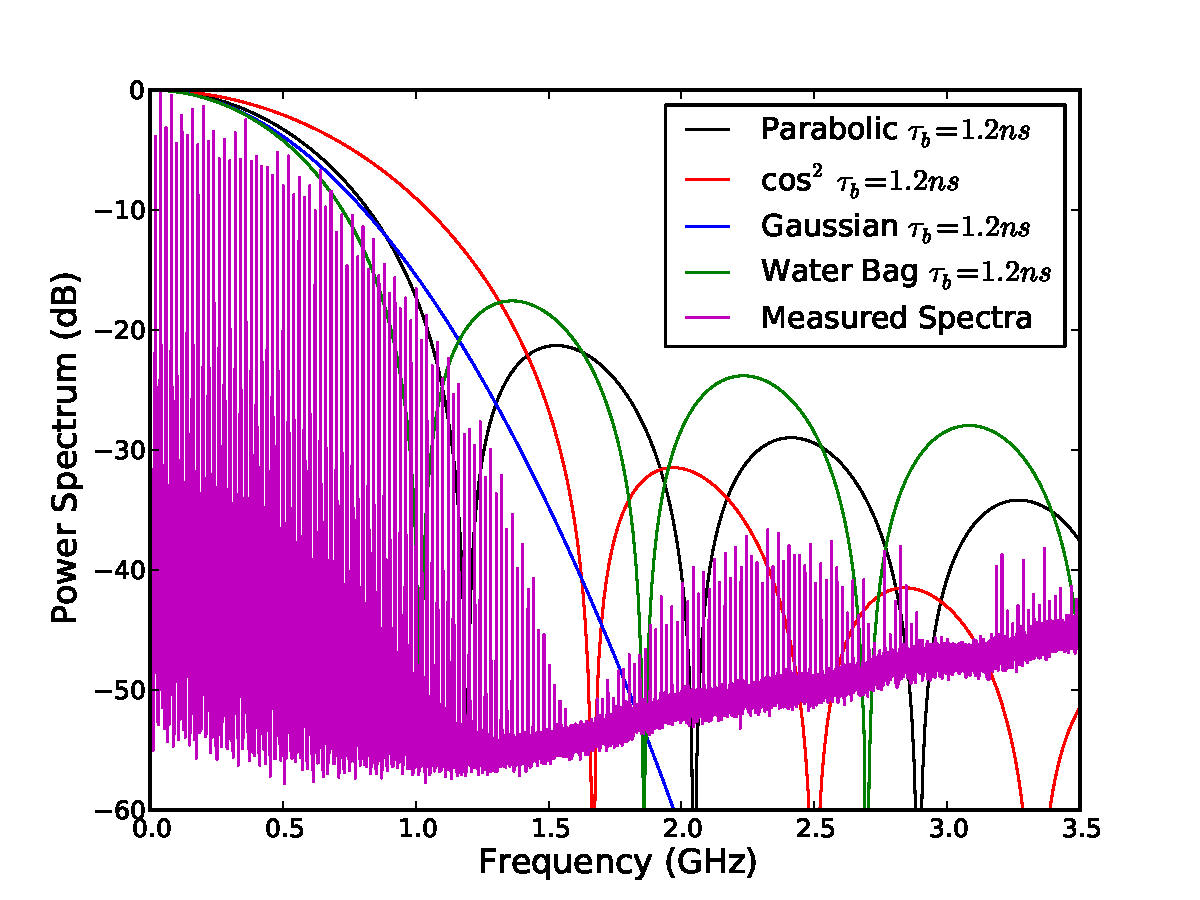
\includegraphics[width=0.65\textwidth]{Wakefields_and_Impedances/figures/beam_spectra_power_12ns.pdf}
\end{center}
\label{fig:power_all}
\caption{A comparison of a measured beam power spectrum and a number of analytical bunch profiles assuming a bunch length of 1.2ns.}
\end{figure}



% Introduce a number of longitudinal profiles in time domain - gaussian, parabolic line density, cos^2, water bag - comments of realism (gaussian being infinite) - truncated gaussian
% Comparison in the frequency domain - firstly gaussian compared to truncated gaussian - infinite tails reduce the magnitude of the higher frequency components and lobe
% Gaussian, parabolic, cos^2 - all with the same bunch length
% Using the above examples try using a number of different bunch lengths to illustrate how they change (gaussian - just extends further, parabolic, cos^2 lobe frequency changes)
% Finally - comparison to measured spectra to illustrate changes in bunch length and frequency components as bunch is ramped and squeezed

\section{Beam induced heating due to a low Q impedance}

For an impedance with a characteristic Q that is small (Q $<$ 10), it can be seen that the impedance peak will interact substantially with a number of beam harmonics (see Fig.~\ref{fig:low_q_harmonics}) due to the broad frequency range it occupies.

\begin{figure}
\begin{center}
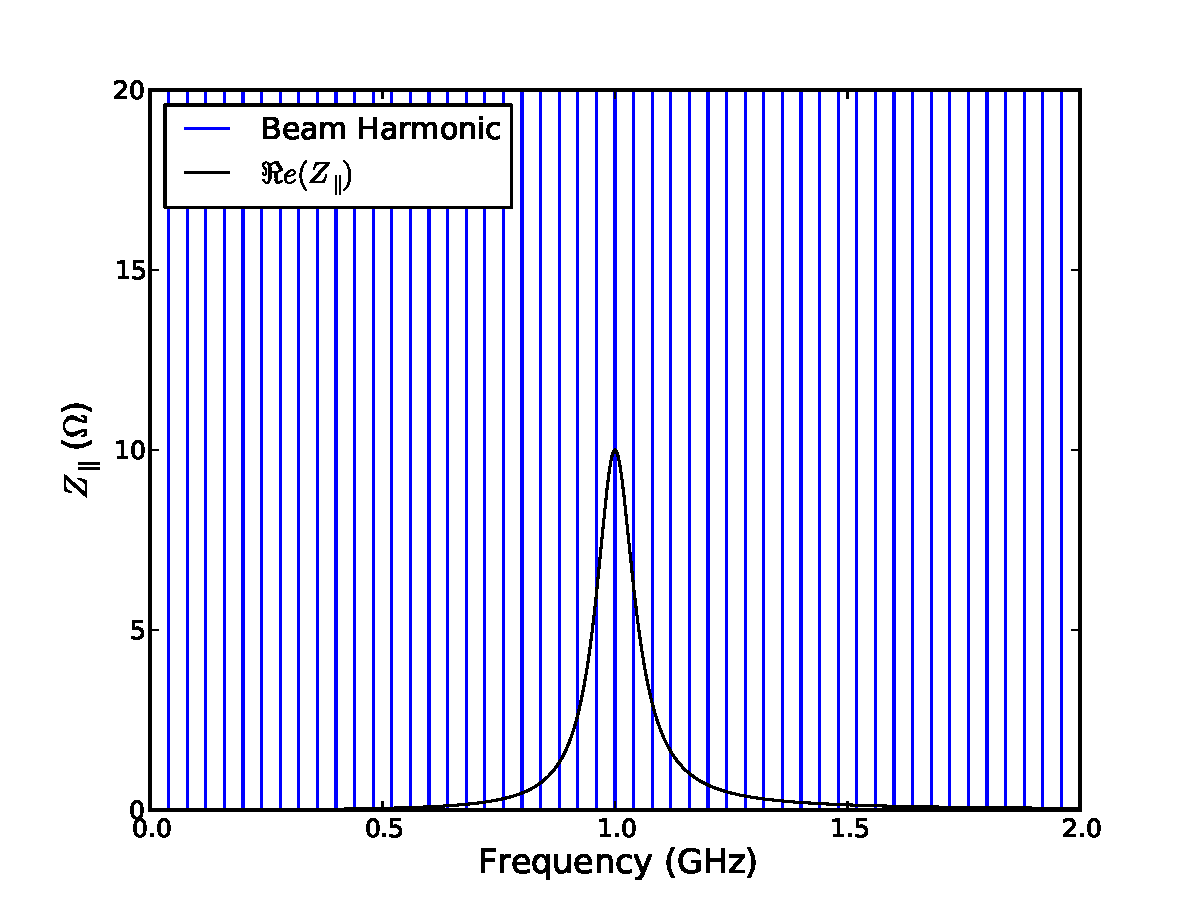
\includegraphics[width=0.65\textwidth]{Wakefields_and_Impedances/figures/low_q_10_resonance_beam_harmonics.pdf}
\end{center}
\label{fig:low_q_harmonics}
\caption{The beam harmonics of a beam with a bunch spacing of 25ns overlayed on the real component of the longitudinal impedance an example of a low Q impedance ($R_{s}=10\omega$, Q = 10, $f_{res}=1GHz$). The blue lines represent the frequency of a beam harmonic, not necessarily the magnitude of the power spectrum at that point. Note that a number of beam harmonics overlay non-zero impedance values.}
\end{figure}

Further investigation of the longitudinal beam spectrum reveals that there is significant structure between the major harmonics (which are due to the bunch spacing of the beam) which can be attributed to the other time structures of the beam, for example the bunch train spacing, or the interval between the pilot bunch train and the subsequent bunch train. As such the treatment of the estimation of beam losses requires a broad spectrum approach. If we consider Eqn.\ref{eqn:power_loss_omega} we see that we can treat the power losses in an integral form. We can observe a number of properties using this assumption. The power loss is proportional to the beam properties in the following manner:

\begin{enumerate}
\item{$P_{loss} \propto N^{2}$}
\item{$P_{loss} \propto n_{bunch}$}
\end{enumerate}

\section{Beam induced heating due to a high Q impedance}

In contrast to the overlap of the beam spectrum with a low Q impedance, for a high Q impedance only one beam harmonic lies upon the resulting impedance to any significant quantity. This is illustrated in Fig~\ref{fig:high_q_harmonics} If we consider Eqn \ref{eqn:heating-gen} and consider the situation where

\begin{equation}
\left( 2 \left| \lambda \left(p \omega_{rev}n_{bunch} \right)  \right|^{2}  \Re{}e \left( Z_{\parallel} \left(p \omega_{rev}n_{bunch}\right) \right) \right) = 
\begin{cases}
\left( 2 \left| \lambda \left( \omega_{res} \right)  \right|^{2}  \Re{}e \left( Z_{\parallel} \left( \omega_{res} \right) \right) \right) &\textrm{if $p \omega_{rev} n_{bunch} = \omega_{res}$}\\
0								&\textrm{if $p \omega_{rev} n_{bunch} != \omega_{res}$}
\end{cases}
\label{eqn:single_harmonic_profile}.
\end{equation}

\begin{figure}
\begin{center}
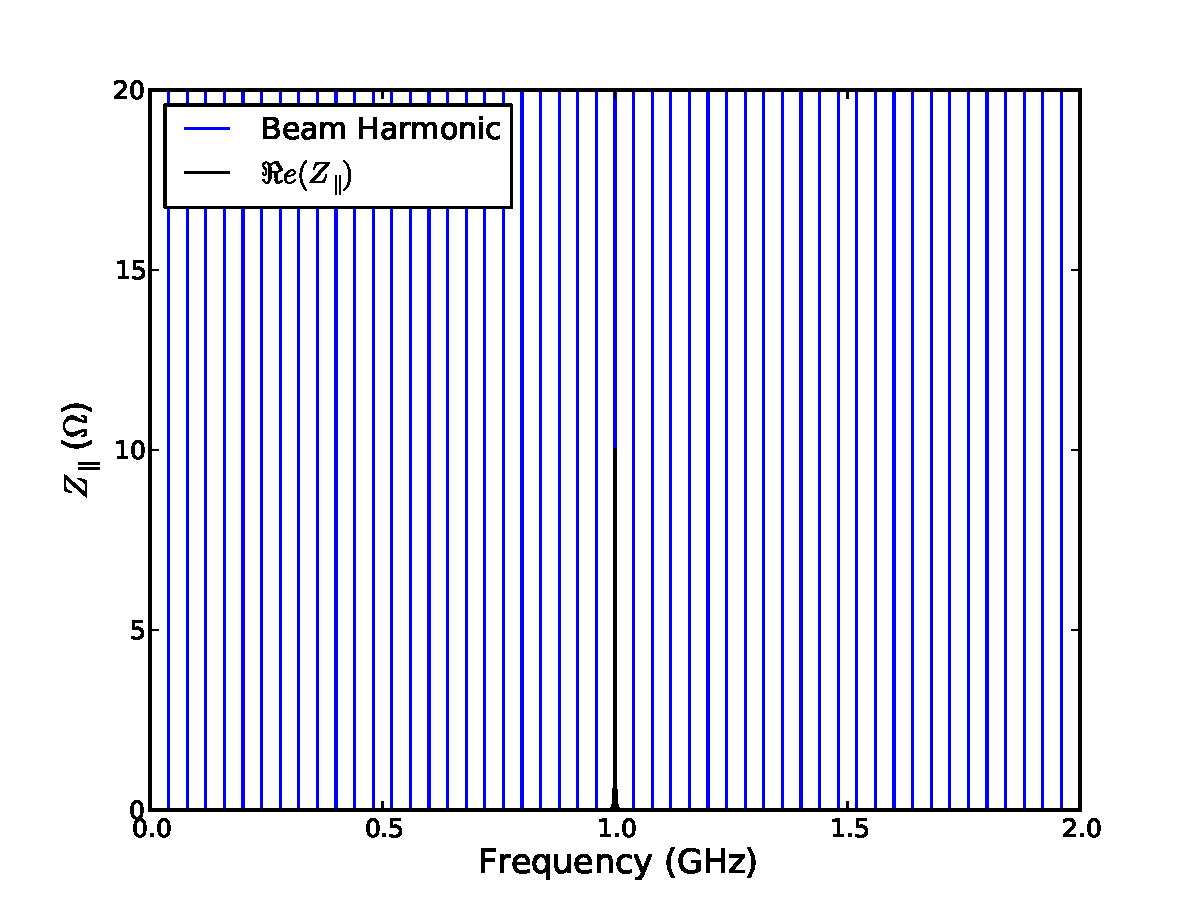
\includegraphics[width=0.65\textwidth]{Wakefields_and_Impedances/figures/high_q_1000_resonance_beam_harmonics.pdf}
\end{center}
\label{fig:high_q_harmonics}
\caption{The beam harmonics of a beam with a bunch spacing of 25ns overlayed on the real component of the longitudinal impedance an example of a high Q impedance ($R_{s}=10\omega$, Q = 1000, $f_{res}=1GHz$). The blue lines represent the frequency of a beam harmonic, not necessarily the magnitude of the power spectrum at that point. Note that only a single beam harmonic overlays a non-zero impedance values.}
\end{figure}

It can then be seen that Eqn~\ref{eqn:heating-gen} simplifies to

\begin{equation}
P_{loss} = \left( \omega_{rev}eN_{b}n_{bunch}  \right)^{2}  \left( 2 \left| \lambda \left( \omega_{res} \right)  \right|^{2}  \Re{}e \left( Z_{\parallel} \left(\omega_{res} \right) \right) \right). 
\label{ean:heating-high-q}
\end{equation}

The following properties can subsequently be seen as a result:

\begin{enumerate}
\item{$P_{loss} \propto N^{2}$}
\item{$P_{loss} \propto n_{bunch}^{2}$, provided that the resonant frequency of the resonance continues to coincide with a beam harmonic.}
\end{enumerate}

\section{Some Examples of the Beam-Induced Heating}

In this section we shall illustrate some important factors that have been covered in previous sections. In particular, the interaction of different bunch profiles at different bunch lengths with an example cavity resonance will be covered in some detail to illustrate how the estimated heating can change drastically depending on higher frequency lobes in the beam current spectrum. In addition, the heating due to two particle beams in the same vacuum chamber shall be briefly covered for interest.

\subsection{The Effect of Bunch Length on Power Loss}

As can be seen in Figs.~\ref{fig:freq_dom_prof} and \label{fig:diff_bunch_len_para}, the bunch profile and the bunch length can significantly alter the magnitude of the beam current at higher frequencies. To illustrate this, let us consider two resonant impedances, one broadband $Z_{bb}$ and one narrow band $Z_{nb}$ impedance, characterised by having a low-$Q$ and a high-$Q$ respectively. Both impedances shall have the same resonant shunt impedance $R_{s} = 100\Omega$. The broadband impedance shall have a $Q_{bb}=1$, and the narrow band impedance $Q_{nb}=1000$. The resonant frequency will be changed to illustrate effects in different regimes of the bunch length and of different bunch profiles.

We shall use the gaussian bunch profile and the $cos^{2}$ bunch profile for these examples. The gaussian is useful to illustrate the effect of just the changing bunch length, and the $cos^{2}$ due to the presence of a high frequency lobe in it's frequency domain current spectrum. The $cos^{2}$ frequency domain current profile is given by

\begin{equation}
I \left( \omega \right) = \frac{sin \left( \omega \tau_{b}/2 \right)}{ \omega \tau_{b}/2 \left[ 1 - \left(  \omega \tau_{b}/2 \right)^{2}  \right]}.
\end{equation}

First we shall consider a narrowband impedance which has a resonant frequency $\omega_{0} =2GHz$ which falls upon a beam harmonic such that $\omega_{0}=n\omega_{rev}$ where n is an integer. It should be noted that for other cases the contribution of these sources of heating is negligible due to the small beam current at this frequency. There are two extreme cases; that of  $\omega_{0} \gg 1/\tau_{b}$, in which it can be seen that the current spectrum will be negligible at the frequency of the impedance, and $\omega_{0} \ll 1/\tau_{b}$ where the beam current spectrum is essentially the same as the DC spectral component. The transition in this intervening regime is shown in Fig~\ref{fig:bunch_length_heat_narrow}, assuming a bunch current of 1A. It can be seen that in this case the heating falls drastically as the bunch length increases.

\begin{figure}
\begin{center}
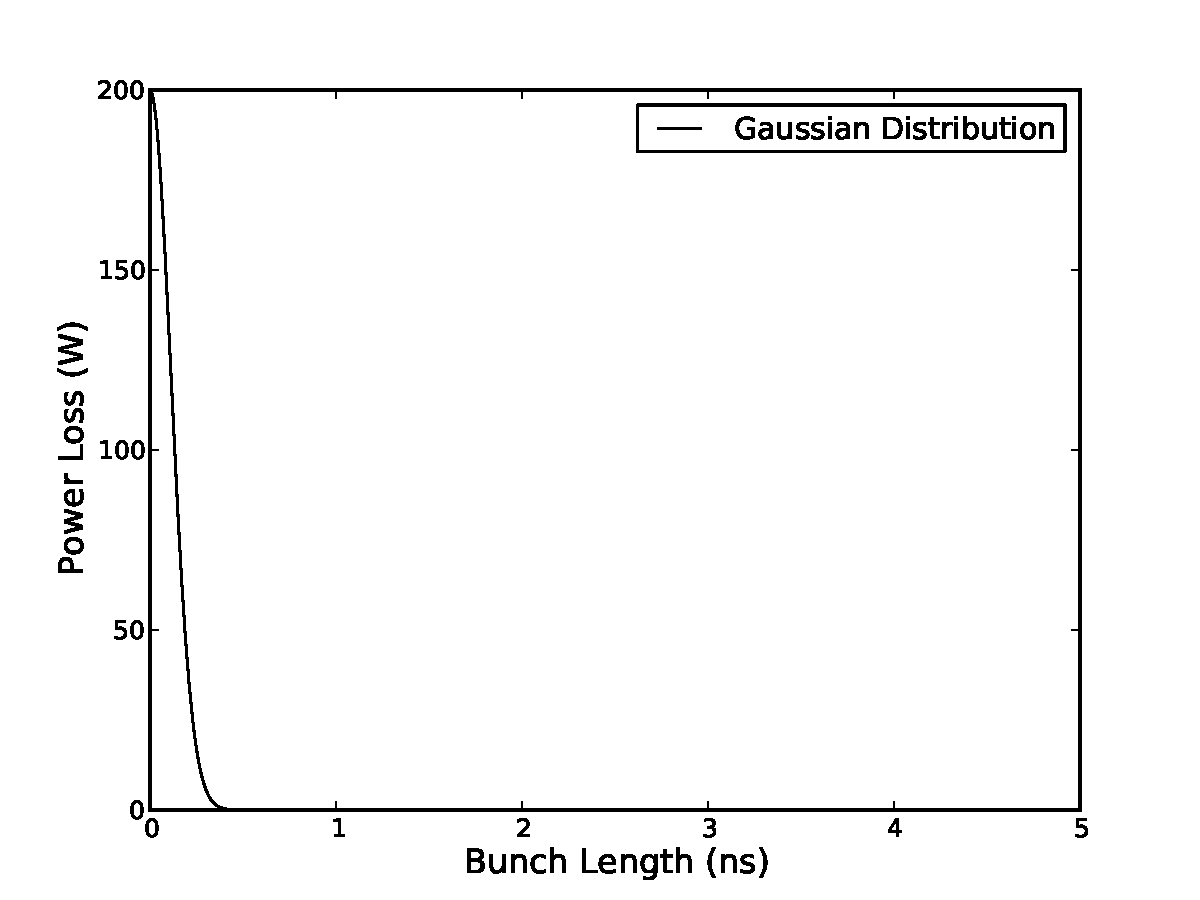
\includegraphics[width=0.8\textwidth]{Wakefields_and_Impedances/figures/heating_narrowband_gauss_bunch_length.pdf}
\end{center}
\label{fig:bunch_length_heat_narrow}
\caption{The change in power loss due to a narrow band resonance characterised by $\omega_{0} = 2GHz$, $R_{s} = 100\Omega$, $Q = 1000$ with a gaussian bunch distrbution of different lengths.}
\end{figure}

If we instead consider a cos$^{2}$ distribution we instead see the effect of the secondary lobes in the beam current spectrum. The power loss with bunch length is shown in Fig.~\ref{fig:bunch_length_heat_narrow_cos} in comparison to that of the gaussian profile. The beam power spectrum for a number of different bunch lengths are shown with the real component of the longitudinal impedance in Fig.~\ref{fig:imp_profile_cos}. Here it can be clearly seen that the intersection of the secondary lobe with the resonant impedance causes a peak in the power lost by the beam, highlighting the neccessity to be aware of the resonant frequencies of resonant impedances with relation to the beam harmonics.


\begin{figure}
\subfigure[]{
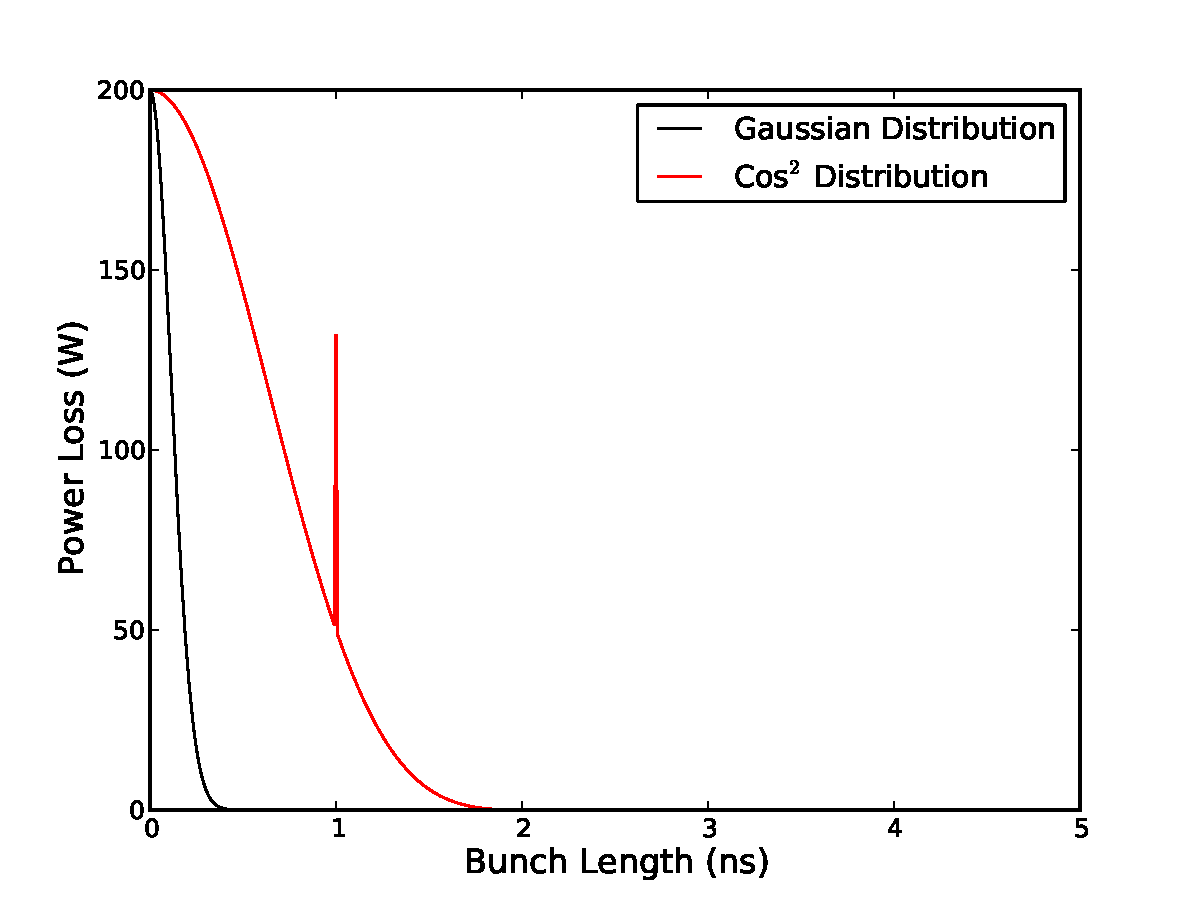
\includegraphics[width=0.5\textwidth]{Wakefields_and_Impedances/figures/heating_narrowband_gausscos_bunch_length.pdf}
\label{fig:long_imp_narrow_current}
}
\subfigure[]{
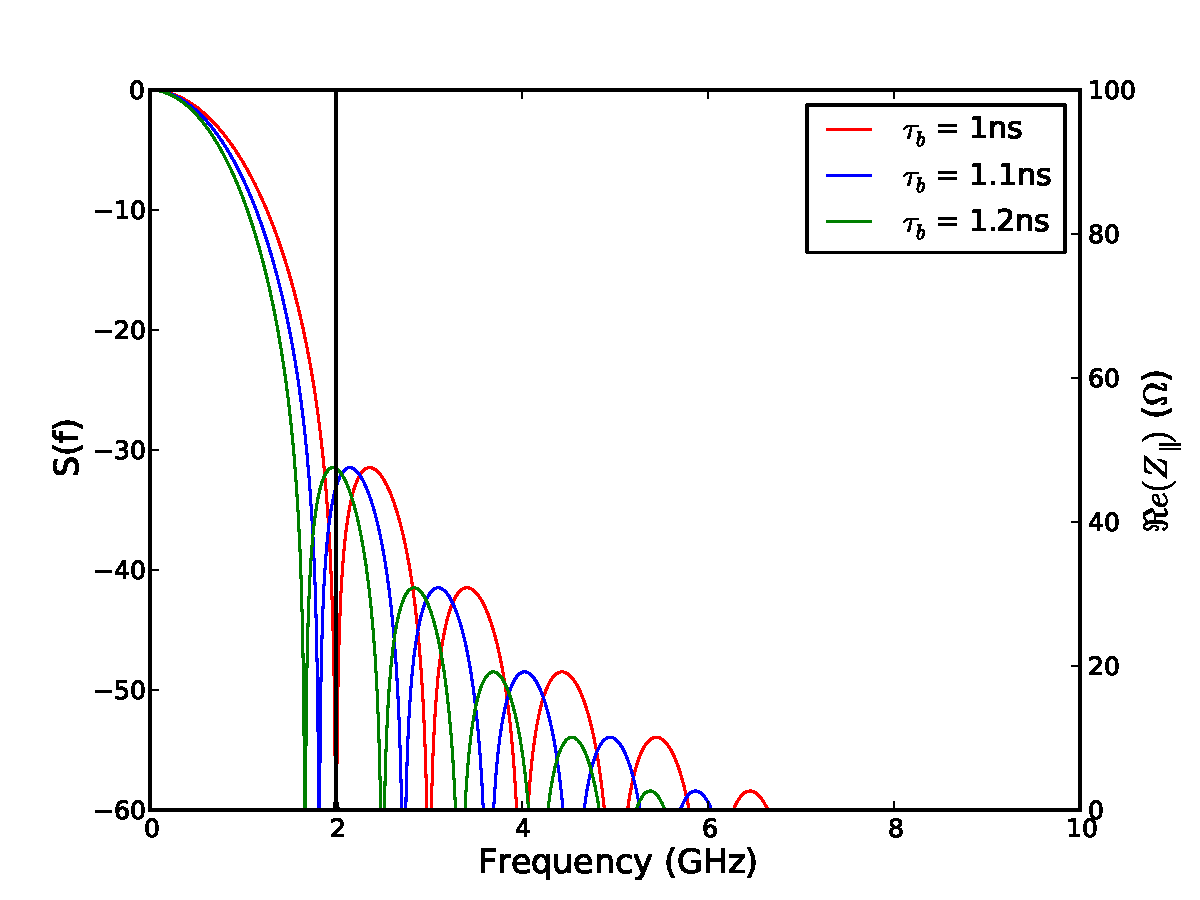
\includegraphics[width=0.5\textwidth]{Wakefields_and_Impedances/figures/impedance_and_power_cos_res.pdf}
\label{fig:imp_profile_cos}
}
\caption{\ref{fig:long_imp_narrow_current} The change in power loss due to a narrow band resonance characterised by $\omega_{0} = 2GHz$, $R_{s} = 100\Omega$, $Q = 1000$ interacting with a cos$^{2}$ bunch distribution with different bunch lengths. The impedance and the beam power spectrum are shown in \ref{fig:imp_profile_cos} to illustrate how this relates to the power loss.}
\end{figure}

For the broadband heating we shall consider a resonant impedance defined by the following parameters, $\omega_{0} = 2GHz$, $Q=1$, $R_{s}=100\Omega$. To account for the multiple beam harmonics that will interact with the resonance, it is assumed that the beam harmonics in this case occur at $20$MHz intervals. The impedance and the beam power spectrum is shown in Fig.~\ref{fig:broadband_heat_bunch_len} and the resulting power loss in Fig.~\ref{fig:broadband_power_loss} where it can be seen that the power loss decreases slowly with increasing bunch length. This is due to the significant contribution to the power loss at low frequencies, in which the component of the beam power spectrum decreases only marginally due to the decreasing bunch length.

\begin{figure}
\subfigure[]{
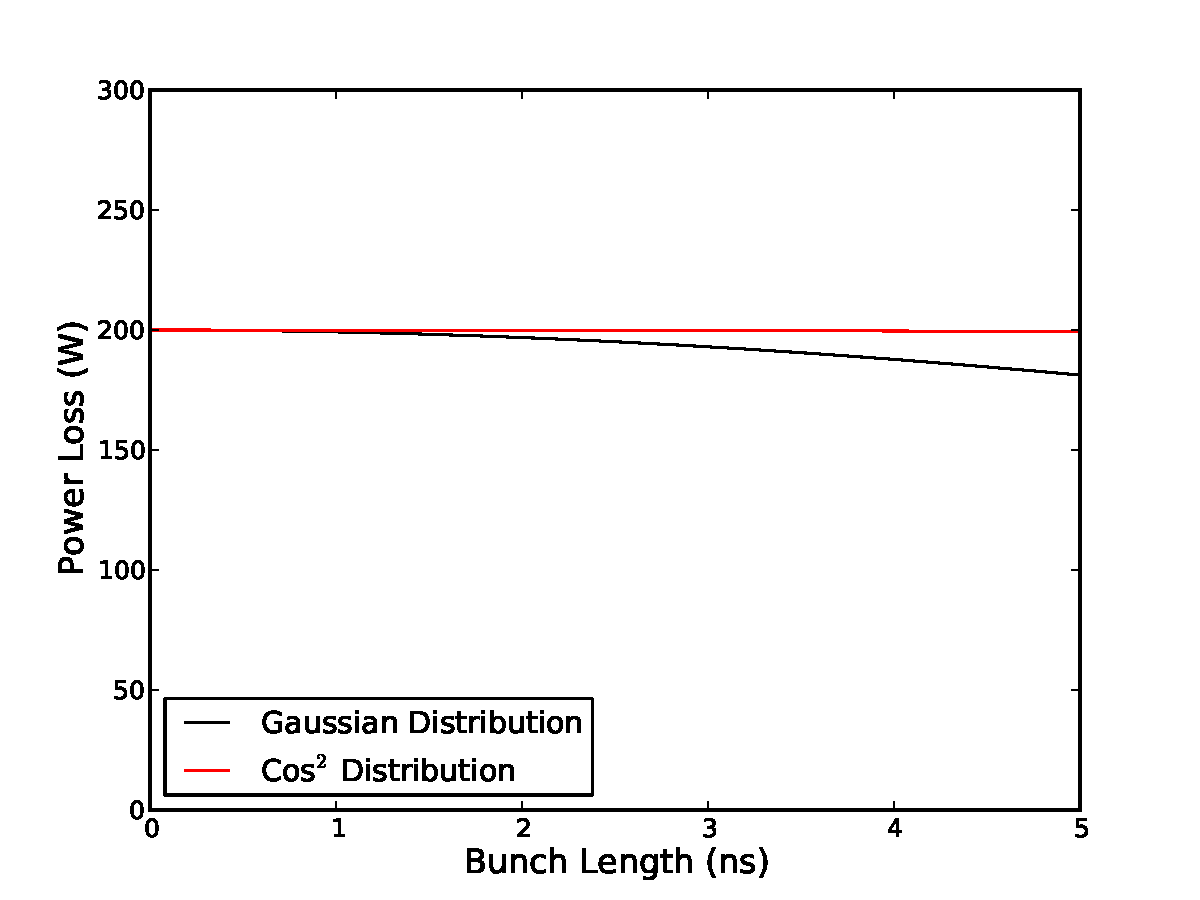
\includegraphics[width=0.5\textwidth]{Wakefields_and_Impedances/figures/heating_broadband_gausscos_bunch_length.pdf}
\label{fig:broadband_heat_bunch_len}
}
\subfigure[]{
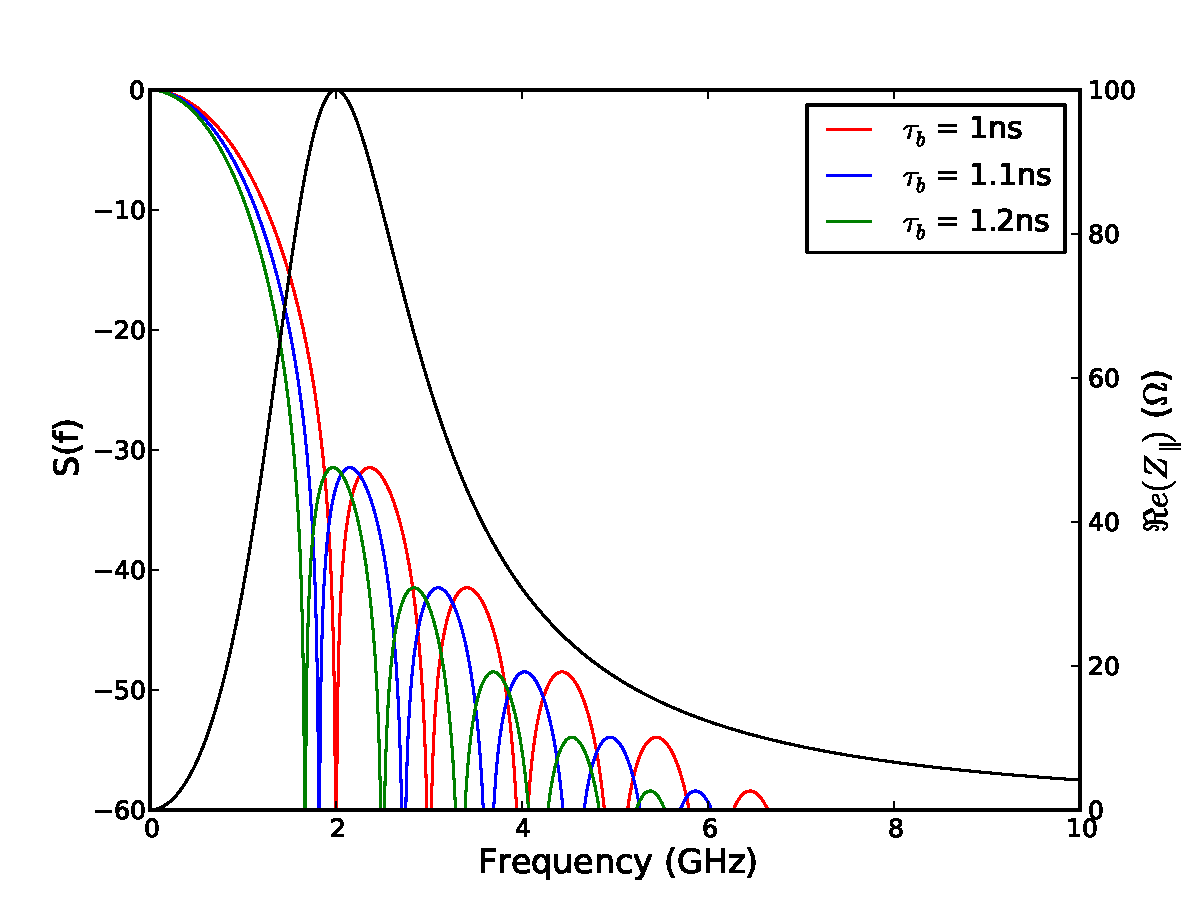
\includegraphics[width=0.5\textwidth]{Wakefields_and_Impedances/figures/impedance_and_power_cos_res_broad.pdf}
\label{fig:broadband_power_loss}
}
\caption{\ref{fig:broadband_heat_bunch_len} The change in power loss due to a narrow band resonance characterised by $\omega_{0} = 2GHz$, $R_{s} = 100\Omega$, $Q = 1$ interacting with a cos$^{2}$ bunch distribution with different bunch lengths. The impedance and the beam power spectrum are shown in \ref{fig:broadband_power_loss} to illustrate how this relates to the power loss.}
\end{figure}

\subsection{Beam-Induced Heating due to two traversing beams}

Previous work [cite A. Grudiev TCTVB/TCLIA] has investigated the effect of two beams in a vacuum on the beam-induced heating. This is restated here for the sake of completeness.

To begin, consider the two currents $I_{b1} = I_{0}e^{i\phi_{1}}$ and $I_{b1} = -I_{0}e^{i\phi_{2}}$ representing two counter rotating beams. $I_{0}$ represents the beam current, and $\phi_{1/2}$ the phase of beam 1 and beam 2 respectively. Each beam also sees a seperate potential when it traverses the impedance, given by $V_{b1} = \int_{b1} E_{z} e^{i\omega_{0}z/c} dz$ and $V_{b2} = \int_{b2} E_{z} e^{i\omega_{0}z/c} dz$ respectively. By Ohms law it can then be seen that

\begin{equation}
\begin{pmatrix}
V_{b1} \\
V_{b2}
\end{pmatrix}
=
\begin{bmatrix}
Z_{11} & Z_{12} \\
Z_{21} & Z_{22}
\end{bmatrix}
\begin{pmatrix}
I_{b1} \\
I_{b2}
\end{pmatrix}.
\end{equation}

The power loss due to both beams can then be seen to be

\begin{equation}
P_{loss} = \begin{pmatrix}
V_{b1} & V_{b2}
\end{pmatrix}
\begin{pmatrix}
I_{b1} \\
I_{b2}
\end{pmatrix}^{*}.
\end{equation}

In the worst case scenario, the values of the impedance matrix are real, and are equal in value to the peak values of the resonant impedance
\begin{equation}
Z_{11} = 2R^{b1}_{s};\text{    } Z_{22} = 2R^{b2}_{s};\text{    }  Z_{12} = Z_{21} = 2 \sqrt{R^{b1}_{s}R^{b2}_{s}}.
\end{equation}

The power loss then becomes

\begin{equation}
P_{loss} = I_{0}^{2} 2 \left( R_{s}^{b1} +  R_{s}^{b1} - 2\sqrt{R^{b1}_{s}R^{b2}_{s}} cos \left( \delta \phi \right) \right)
\end{equation}

where $\delta \phi = \phi_{1} - \phi_{2}$ is the phase difference between beam 1 and beam 2. This can be found relatively easy by comparing the distance $\delta s$ from a collision IP of the machine. Assuming the beams are ultrarelativistic $\delta \phi = \omega_{rev} 2  \delta s /c$. It can then be seen that the the last term may either reduce or increase the power loss depending on whether $cos\left( \delta \phi \right) = 1$ or $cos\left( \delta \phi \right) = -1$ respectively.


\subsection{Beam Instabilities}

Beam Instabilities is the collective term for a various group of mechanisms which attribute to the degradation of beam properties during the circulation of a beam within a synchrotron. These can typically be into a number of different subgroups, summarised below:

\begin{enumerate}
\item{Coherent Effects - Occuring due to the bulk oscillation of the bunch(es)}
\item{Incoherent Effects - Occuring due to a mechanism that effects particles dependent on their position within in the bunch}
\item{Single-Bunch - Occuring only on the scale of a single bunch}
\item{Multi-Bunch - Occuring due to coupling of the motion between multiple bunches}.
\end{enumerate}

The mechanisms driving these instabilities are multitudinous and of which beam coupling impedance is just one. Others include space charge effects (both direct and indirect)[cite], beam-beam interactions [cite], electron cloud [cite], IBS [cite] amongst others. Here we shall give a brief overview of how these effects cause a degradation in beam operation.

\subsubsection{Tune Shift and Tune Spread} 

As seen in Sec. [ref introduction transverse motion], the transverse equation of motion can be viewed as an oscillatory system. If the particles experience an additional force $ F^{pert}_{x}$ due an external mechanism, not due to the machine optics, it's equation of motion (in the horizontal plane, for example) can be written as

\begin{equation}
\frac{d^{2}x}{ds^{2}} + \left(\frac{Q_{0,x}}{R}\right)^{2} x = \frac{F^{pert}_{x}}{\beta^{2} E_{total}}.
\end{equation}

This subsequently leads to a perturbed oscillation frequency, characterised by the equation

\begin{equation}
\frac{d^{2}x}{ds^{2}} + \left(\frac{Q_{0,x}+ \Delta Q_{pert,x}}{R}\right)^{2} x = 0.
\end{equation}

where $\Delta Q_{pert,x}$ is the part of the betatron frequency caused by the perturbing force. The perturbed tune may also be subsequently be further divided into coherent (the motion of the bunch centroid) and incoherent (motion of individual particles), such that $\Delta Q_{pert,x} = \Delta Q^{coh}_{pert, x} + \Delta Q^{incoh}_{pert, x}$. This seperation leads to the creation of a tune spread in a machine, in which the tune of the beam covers an area of the tune diagram as shown in Fig.~\ref{fig:tune_diag_tune_shift}. In this case particles may be lost when this tune shift causes them to lie upon a major resonance of the beam optics, there by causing cpherent oscillation growth and ultimately particle loss. This leads to negative effects such as emittance growth and lower beam lifetimes.

\begin{figure}
\caption{A tune diagram illustrating the unperturbed tune of a machine, and the resulting perturbed tune and the tune spread as a result of an impedance source. Note that the tune spread has caused some particle to lie upon a major resonance harmonic.}
\label{fig:tune_diag_tune_shift}
\end{figure}

\subsubsection{Longitudinal Single Bunch Instabilities}

Similar to the change in the equations of motion for transverse particles, considering the induced fields in the longitudinal plane produces a perturbation in the longitudinal motion also. This can be thought of as an additional force alongside the electromagnetic force applied by the accelerating cavities. This leads to two interesting phenomenon; potential well distortion, occuring at bunch intensities below some stability criteria, and longitudinal mode coupling instability, or LMCI, above some stability criteria.

The potential well distortion is a direct effect of the incoherent synchrotron tune shift (again, similar in nature to the tune shifts experienced in the transverse plane), which is responsible for a growth in the stable emittance of the bunch. This reveals itself from measurements by a change in the bunch length with increasing bunch intensity, as shown in Fig.~\ref{fig:pot_well_dist}. It should be noted that depending on the source of impedance, the bunch length may increase or decrease depending on whether the bunch is above or below the transition energy of the accelerator.

\begin{figure}
\caption{The change in the bunch length of a proton beam in an SPS like machine due to the effects of a broadband resonator impedance (). Note that the bunch length increases when the beam is above transition, and decreases below transition, as the bunch intensity is increase}
\label{fig:pot_well_dist}
\end{figure}

LMCI occurs when a certain intensity threshold is crossed in the accelerator, leading to a regime known as \emph{turbulent bunch lengthening}. In this mechanism the eigenfrequencies of the natural modes of oscillation of the particles within the RF bucket are shifted due to the changing potential due to the induced wakefield. In high intensity bunches two neighbouring modes may have their frequencies shifted to such an extent that the modes merge into one, thus leading to a case where the modes no longer have only a damped solution, but also a exponentially growing solution. This subsequently leads to the bunch oscillations becoming unstable.

\subsubsection{Transverse Single Bunch Instabilities}

In the transverse plane a number of instability mechanisms apply, which maybe seperated into two forms, those that occur on a time scale much shorter than the synchrotron period, and those that occur on a longer time scale than the synchrotron period. In both cases the leading particles of the bunch, often called the head of the bunch, drives and oscillation in the end, or tails of the bunch. This gives these instabilities their names, the fast head-tail instability, or transverse mode coupling instability (TMCI) and the head-tail instability.

In the case of the fast head-tail instability, the are a number of transverse oscillation modes (see Fig.~\ref{fig:trans_oscillations} for examples), which as with the LMCI experience some frequency shift due to the presence of a wakefield. If the shift is large enough, two of these modes may again couple together, causing an exponential growth of the transverse size of the bunch to occur.

\begin{figure}

\caption{Examples of a number of modes of transverse oscillation. Note that radial and azimuthal modes may occur, as may coupled modes in which the motion of the horizontal and vertical planes is coupled.}
\label{fig:trans_oscillations}
\end{figure}


In the case of the head-tail instability, the movement of a particle from the head of the bunch to the tail and vice versa become important in determining the rate of growth of any unstable modes, and whether any stabilisation mechanisms have sufficient time to damp the growth. This means that the chromaticity of the beam now takes on a great importance, as this relates the betatron tune to the longitudinal motion. This leaves the option of changing the chromaticity of the beam to act as an additional stability mechanism.

\subsubsection{Coupled Bunch Instabilities}

In addition to single bunch instabilities, it is possible in machines where multiple bunches circulate, and possessing wakefields that do not damp in the spacing between bunches (typically caused by high Q resonant impedances), that the motion of the bunch centroids themselves may become coupled together, thus driving what are called coupled bunch instabilities (TCBI for the transverse plane, LCBI for the longitudinal plane). 

This can be understood by imagining the bunch train as a possessing M bunches. This train will then have M possible modes of oscillation with a characteristic frequency of $\omega_{M}$, which may be driven by an impedance at some frequency $\omega_{0}$. If $\omega_{0} \approx n\omega_{M}$ where n is an integer, then the wakefield due to the impedance may drive the oscillation either in a damped fashion (wakefield is out of phase with the oscillation of the mode) or an anti-damped fashion (wakefield is in phase with the oscillation of the mode). In the latter case, this driven oscillation may cause particle losses unless the oscillation is damped via an external mechanism, such as Landau damping or the use of a damper. This motion can occur in both the longitudinal and transverse planes of motion.



\chapter{Beam Based Measurements of Beam Coupling Impedance}
\section{Longitudinal Beam Impedance Measurements}


\subsection{Potential Well Distortion with Bunch Intensity}

The equation for the longitudinal motion of a charged particle in an RF bucket can be linearised and solved to find the so called incoherent synchrotron frequency, that is it's oscillation in energy and phase, given by,

\begin{equation}
\omega_{s} = \frac{\omega_{RF}}{\beta} \left( \frac{\eta V_{T}cos\bar{\phi}}{2\phi E/e}  \right)^{\frac{1}{2}}
\label{eqn:syn_volt}
\end{equation}

where $\omega_{RF} = h\omega_{0}$ is the RF frequency, $\omega_{0}$ is the revolution frequency, h is the harmonic
number of the RF, $\eta = \alpha_{c} - \gamma^{-2}$ is the slip factor, $\alpha_{c} = \gamma_{t}^{-2}$ is the momentum compaction factor, $\gamma_{t}$ is the transition energy gamma factor, $E=\gamma E_{0}$ is the total particle energy, $E_{0}$ is the rest eergy of the particle, $\bar{\phi}$ is the stable phase angle and $V_{T}$ is the total voltage seen by the beam. For an empty bucket (i.e. no particles present) the voltage present is just that of the RF voltage $V_{RF}$ , giving an associated synchrotron frequency $\omega_{s0}$. We can subsequently see from Eqn.~\ref{eqn:syn_volt} that we have the ratio

\begin{equation}
V_{T} = V_{RF}\left(  \frac{\omega_{s}}{\omega_{s0}} \right)^{2}.
\label{eqn:volt_emit}
\end{equation}

Additionally the bunch length L and the energy spread of the bunch $\Delta E/E$ can be shown to be related by

\begin{equation}
L = \frac{\left| \eta \right|c}{\beta\omega_{s}}\frac{\Delta E}{E}
\end{equation}

within the linear approximation. If we assume that the emittance of the bunch is preserved (usually the case in a proton machine), i.e. $L\Delta E = constant$, Eqn.~\ref{eqn:volt_emit} leads to

\begin{equation}
L^{2}\omega_{s} = L_{0}^{2}\omega_{s0}.
\end{equation}

The resulting induced voltage of the bunch depends heavily on the nature of the impedance on which the beam interacts with. In this case we shall illustrate the characteristics of the bunch lengthening with a simple inductive impedance ($Z = j\omega L$). More examples and detail can be found in Ref [B. zotter]. The voltage induced by a bunch with a parabolic line density through a purely inductive impedance is gives a resulting synchrotron frequency given by

\begin{equation}
\omega_{s}^{2} = \omega_{s0}^{2}\left[ 1 - \frac{C}{B^{3}} \frac{I_{b}}{hV_{RF}cos\bar{\phi}} \left( \left| \frac{Z}{n}  \right| - \frac{gZ_{0}}{2\beta\gamma^{2}}   \right)    \right]
\end{equation}

where $c = \frac{3}{\pi^{2}}$ is a constant dependent on the bunch profile, $B = \frac{L}{\pi R}$ is the bunching
factor, given by the ratio of the bunch length to the machine circumference, $I_{b}$ is the bunch current, $g = 1 + 2ln\left(\frac{b}{a} \right)$ is the direct space charge factor, $b$ is the beam pipe radius, $a$ is the beam radius and $Z_{0} = 377\Omega$ is the impedance of free space.

If we consider an ultrarelativistic beam ($\gamma \rightarrow 1$), the space charge factor $g = 0$. Then, considering the value of $\bar{\phi}$ (i.e. whether the bunch is above transition $cos\bar{\phi} > 0$, or below transition $cos\bar{\phi} < 0$), the bunch length increases with the increased bunch current above transition, and decreases below transition. All variables other than $Z/n$ may be measured directly using various instrumentation.

Generalisation of this method to a general complex impedance shows that it is the imaginary component of the longitudinal impedance that contributes the induced voltage, thus being the component of the impedance measured using this method.

\subsection{Synchronous Phase Shift}

As discussed in Section [ref beam induced heating], a particle circulating in circular accelerator losses energy due to interacting with impedances in the machine. If the particle is not undergoing acceleration, it can be seen that to keep the same energy, the particle must have a phase relative to the RF that ensures that the energy losses due to wakefields are equal to the energy gained during the traversal of the RF cavities, given by the equivalence of the energy gain by transit and the energy loss by traversal,

\begin{equation}
U = qeVsin\phi
\end{equation}

where $U$ is the total energy lost by a particle per turn, $q$ is the unit charge, $e$ is the electron charge, $V$ is the RF voltage amplitude and $\phi$ is the synchronous phase. The total energy lost is the sum of all energy losses in the machine, given by

\begin{align}
U & = -e^{2}N_{b}k \\
   & = -e^{2}N_{b}\displaystyle\sum\limits_{n} k_{n} \\
   & = -e^{2}N_{b}\displaystyle\sum\limits_{n} \Re{}e\left( Z_{\parallel,n}\left( \omega \right) \right)\left| \lambda \left( \omega \right) \right|^{2} d\omega
\end{align}

where $k_{n}$ is the kick factor of device n in the accelerator and $ Z_{\parallel,n}$ is the longitudinalimpedance of device n. It can be seen that this allows the measurement of the impedance of the whole device. In addition where the movement of a device is permissible and can be carried out during operation (in collimation systems or insertion devices for example) it is possible to determine the impedance of specific devices by the change in their contribution to the total kick factor. Examples of this measuring method can be found in [ref energy loss of a single bunch in the sps, TDI measurements BS and J]

\section{Transverse Beam Impedance Measurements}


For a bunch interacting with a transverse impedance there are two commonly used methods of measuring the transverse impedance - the variance of the coherent betatron tune shift with bunch intensity and the change of growth/decay rate of head tail instabilities with the chromaticity of the beam [ref Sacherer, Zotter].

When a bunch is exposed to a tranverse inmpedance $Z_{\perp}$, it undergoes a complex frequency shift in in betatron frequency


\begin{equation}
\Delta{}\omega_{\beta} = \frac{N_{p}ec}{4\sqrt{\pi}\omega_{\beta} \left( E/e \right)T_{0}\sigma_{t}} i\left( Z_{\perp} \right)_{eff}
\label{eqn:complex_tun_shift}
\end{equation}

where $N_{p}$ is the number of particles in the bunch, $E$ is the energy, $T_{0}$ is the revolution frequency, $\sigma_{t} = \sigma_{z}/c$ is the bunch length, $\omega_{\beta} = 2\pi{}Q f_{rev}$ is the betatron frequency and $\left( Z_{\perp} \right)_{eff}$ is the effective transverse impedance. This is given by the impedance convolved with a weighting function h which is determined by the longitudinal bunch profile given by

\begin{equation}
\left( Z_{\perp} \right)_{eff} \left( \omega_{\xi} \right) = \int_{-\infty}^{\infty} Z_{\perp} \left( \omega \right) h){m} \left(  \omega - \omega_{\xi} \right) d\omega.
\end{equation}

As an example, for the 0-mode coherent bunch oscillation and assuming a gaussian bunch profile the weighting function can be written as

\begin{equation}
h_{0} \left( \omega \right) = \frac{\sigma_{t}}{\sqrt{\pi}}e^{ \left(  \omega \sigma_{t}  \right)^{2}}.
\label{eqn:weighting_func}
\end{equation}

It can be seen from Eqn.~\ref{eqn:weighting_func} that the function is centred on $\omega_{\xi}$ which is dependent on the chromaticity $\xi$ (see section[insert]) and the phase slip factor $\eta$ as

\begin{equation}
\omega_{\xi} = \xi \frac{\omega_{\beta}}{\eta}.
\end{equation}

Eqn~\ref{eqn:complex_tun_shift} indicates that the imaginary component of the effective transverse impedance contributes to a real coherent tune shift, which the real component to an imaginary tune shift, visible as a growth/decay time in the oscillation. For a broadband impedance ($Q=1$), at low frequencies it is possible to assume that $\Im{}m\left(  Z_{\perp} \right) \approx const.$ It then follows that this is directly proportional to the real tune shift which can be obtained by measuring the coherent tune as a function of bunch intensity.

\subsection{Tune shift change with bunch intensity}

The real component of the solution to Eqn~\ref{eqn:complex_tun_shift} can be related to the integer betatron tune by

\begin{equation}
\Delta Q = \frac{\Omega - \omega_{\beta}}{\omega_{0}} \approx \frac{1}{\omega_{0}} \frac{N_{p}ec^{2}}{4\sqrt{\pi}\omega_{\beta} \left( E/e \right)T_{0}\sigma_{t}} \Im{}m\left(  Z_{\perp} \right)_{eff},
\end{equation} 

where $\Omega$ is the measured betatron frequency. It can easily be seen that by altering the bunch population the tune shift $\Delta Q$ can be measured also and subsequently the value for $\Im{}m\left(  Z_{\perp} \right)$ can be obtained.

\subsection{Growth time change with chromaticity}

Similarly to the tune shift measurements, we consider the imaginary component of the solution. Similarly to a harmonic oscillator, the imaginary part of the solution denotes a damping time of the oscillation, $\tau$, in this case given by

\begin{equation}
\frac{1}{\tau} = -T_{0} \frac{N_{p}ec^{2}}{4\sqrt{\pi}\omega_{\beta} \left( E/e \right)T_{0}\sigma_{t}} \Re{}e\left(  Z_{\perp} \right)_{eff}.
\end{equation}

$\Re{}e\left(  Z_{\perp} \right)_{eff}$ is dependent only on the chromaticity $\xi$, being zero at $\xi = 0$ and different from zero for other values of chromaticity. Depending on whether the measurements are done above or below transition the produces either a damping for positive chromaticity above transition and growth below transition, and vice versa for negative chromaticity. Further details can be found in.

%%%%%% Bench Top Impedance Measurements %%%%%%

\chapter{Bench Top Measurements of Beam Coupling Impedance}


Due to the sensitivity of the beam coupling impedance to the boundary conditions of the equipment used, it is necessary to utilise different measurement techniques to fully analyse the impedance of accelerator structures.

\section{Low Q-factor Impedances}

For structures that are expected to contain mostly low Q-resonances (i.e. resistive wall impedance) it is appropriate to use the coaxial wire method[ref], sometimes also called the stretched wire method. This method relies on the similarity of the electromagetic field profile due to an ultrarelativistic charged particle and that of a short electrical pulse sent along a coaxial wire. 

An moving charged particle produces an electromagnetic field in a arc transverse to its direction of motion, where the angle of the arc opening is proportinal to the relativistic factor of the particle $\gamma$. For an ultrarelativistic particle ($\gamma \leftarrow \infty$), the field becomes entirely perpendicular to the direction of motion. If we place a conductive wire along the same path we would expect the charged particle to take (in most cases this is well represented by a straight wire), a short electrical pulse sent along this wire would propogate in the TEM (transverse electrical and magnetic field) mode, producing a field profile similar to that emitted by the ultrarelativistic charged particle (see. Fig. \ref{fig:coax-part-profile})


\begin{figure}

\caption{Comparison of the electromagnetic field profile of a moving charged particle and a short time pulse propogating along a coaxial wire.}
\label{fig:coax-part-profile}
\end{figure}

\subsection{Classical Coaxial Wire Method}

The classical coaxial wire method, first proposed by V. Vaccarro in 1990 [ref], is a transmission method that measures the complex transmission coefficient of a DUT (Device Under Test) made up of the equipment whose impedance is to be measured and a coaxial wire passing through it. 

The experimental setup is as shown in Fig. \ref{fig:classic-coax}. Firstly the external circuit (i.e. everything not the DUT) is matched to the characteristic impedance of the coaxial line inside the DUT. This is done by measuring the reflection coefficient $\Gamma$ for the setup with only one port connected to the DUT and the other end terminated by an open connection. Knowing the characteristic impedance of the VNA and associated cables (typically $Z_{0} = 50\Omega$), we can easily calculate the characteristic impedance, $Z_{c}$, from the relation,

\begin{equation}
\Gamma = \frac{Z_{c} - Z_{0}}{Z_{c} + Z_{0}}.
\end{equation}

We then electrically match the characteristic impedance by adding resistors in series just before the DUT to resistively match the characteristic impedance of the VNA to that of the DUT. It is possible to use physical matching also using transition cones but these are costly, time consuming to construct and require new cones for each piecof equipment measured. And as can be seen in Fig. \ref{fig:matching-plot}, matching with a resistor is highly effective at removing the presence of reflections in coaxial measurements.

\begin{figure}

\caption{Experimental setup for a measurement of the beam coupling impedance using the classical coaxial wire method}
\label{fig:classic-coax}
\end{figure} 

\begin{figure}

\caption{An example of a reflection measurement made with and without a matching resistor. The faded line is the measurement without matching, the bold line that with. The reduction in the reflection can be seen.}
\label{fig:matching-plot}
\end{figure}

The value that we wish to measure to evaluate the beam coupling impedance of a device are the scattering parameters of the resulting circuit, in particular $S_{21}$, the normalised transmission parameter through the DUT. $S_{21}$ is calculated by taking the measured transmission parameter $S_{21,DUT}$ and dividing it by the transmission parameter through a reference line of the same physical length as the DUT,

\begin{equation}
S_{21} = \frac{S_{21,DUT}}{S_{21,REF}}
\end{equation}.

The effect of this is to correct the measured phase change in the DUT to be that only caused by the imaginary component of the beam coupling impedance.

There are subsequently a number of ways to evaluate the beam coupling impedance of the DUT depending on it's expected properties. For devices that are expected to have a either a small impedance, or those that are physically very short in length, it is possible to use the so called lumped impedance formula[ref];

\begin{equation}
Z = 2Z_{c} \frac{1-S_{21}}{S_{21}}
\end{equation}.

For distributed impedances, it is suitable to use the so called log formula (called so due to attenuation causing a log function to appear in the evaluation),

\begin{equation}
Z = -2Z_{c} ln \left( S_{21} \right)
\end{equation}.

For long components or measurements at very high frequencies there exists the improved log formula. This takes into account more completely the electrical length of the device, given by

\begin{equation}
Z = -2Z_{c} ln \left( S_{21}  \right) \left( 1 + j\frac{ln \left( S_{21}\right) }{2\Theta}  \right)
\end{equation}

where $\Theta = 2\pi \frac{L}{\lambda}$ is the normalised electrical length of the device, $L$ the length of the device, $\lambda$ the wavelength of the frequency of measurement. It is possible to see that the lumped impedance formula can be used when $\Theta \leq 1$, and the improved log formula becomes useful for $\Theta \geq 5$[erk's paper].




\subsection{Resonator Coaxial Wire Method}

An alternative method for measuring the beam coupling impedance is by using the so called resonator method. The setup for this method is similar to that of the classical coaxial wire method, except that the matching resistor network between the VNA and DUT is replaced by a weak capacitive coupling ($S_{11} < 0.5dB$) at both ends of the DUT. This then produces a structure which resonates at frequencies where the wavelength corresponds to the classical closed structure form,

\begin{equation}
\lambda = \frac{2L}{n}
\end{equation}

where $\lambda$ is the wavelength of the resonance, n the harmonic of the resonance and L the length of the device. 

The resonant method enables accurate measurement of the transmission losses due to the real longitudinal impedance. Additional advantages are that no matching is required, and a large number of mechanical uncertainties (electrical connections, consistency of calibration) can be avoided. However it can be seen that the frequency resolution is limited due to the length of the DUT so the method is not recommended as the only measurement method for structures expected to contain high-Q, narrowband resonances. It can however be used to corroborate the results obtained using the classical method.

For each resonancce peak, the loaded Q-factor and the frequency of the resonance are measured. For a weak coupling at both ends of the DUT, we can write the coupling coefficient k as

\begin{equation}
k = \frac{\left| S_{21} \right|}{1 - \left| S_{21} \right| }.
\label{eqn:coupling_coeff}
\end{equation}

The difference between the unloaded $Q$-factor, $Q_{0}$ , and the loaded $Q$-factor, $Q_{L}$, is a function of k. We can get an approximate correction by using the formula

\begin{equation}
Q_{0} = Q_{L} \left( 1 + k  \right).
\label{eqn:Q_correc}
\end{equation}

Subsequently the measured line attenuation (in Np/m) is then calculated

\begin{equation}
\alpha_{m} = \frac{\pi}{\lambda Q_{0}}.
\label{eqn:atten}
\end{equation}

Note that this attenuation includes both that from the beam coupling impedance due to the finite resistance of the wire material. We can estimate the attenuation due to the wire material as

\begin{equation}
\alpha_{w} = \sqrt{\pi \rho_{w} \epsilon f} \frac{1}{d ln D/d}
\label{eqn:wire_atten}
\end{equation}

where $\rho_{w}$ is the wire resistivity, $\epsilon$ the permitivitty, $f$ the frequency, $d$ the diameter of the inner conductor and $D$ the diameter of the outer conductor. At very low frequencies the finite skin depth of the inner conductor would also have to be taken into account. Using the corrected attentuation $\alpha = \alpha_{m} - \alpha_{w}$, the real longitudinal impedance per unit length can be found to be 

\begin{equation}
\Re e\left\{ Z \right\} = 2Z_{c} \alpha
\label{eqn:res_imp}
\end{equation}

\begin{figure}

\label{fig:res-resonancce-examples}
\caption{An example of the resonance pattern seen whilst performing measurements using the resonant method. Each peak corresponds to one data point in the final measurements.}
\end{figure}

To calculate the imaginary impedance using the resonant method involves a more involved calculation. In particular it is necessary to carry out measurements using the resonant method on a reference pipe of the same physical length to the DUT, either using physical measurements or a simulated measurement.

If we consider the complex impedance of the two measurements, $Z_{DUT}$ for the DUT and $Z_{REF}$ for a perfectly conducting reference pipe, we can simplify them as

\begin{align}
Z_{DUT} & =  R + jX_{1}  =  Z_{1}e^{j \phi} \\
Z_{REF} & =  jX_{2}  =  Z_{2}e^{j.0}
\end{align}

where $R$ is the resistive component of the DUT impedance, $X_{1/2}$ the imaginary component of the impedance (DUT and reference pipe respectively), $\phi$ is the angle of DUT impedance projected onto a complex plane and $Z_{2} = \sqrt{R^{2} + X^{2}}$. If we consider a measured value depedent on the impedance, for example the transmission parameter $S_{21}$ at a resonance peak, we have the following relations

\begin{align}
S_{21}^{DUT} = S_{0}e^{j \left( \omega_{1}t + \phi \right)} \\
S_{21}^{REF} = S_{0}e^{k \left( \omega_{2}t \right)}
\end{align}

where $S_{0}$ is some normalised scalar, $\omega_{1/2}$ is the frequency of the resonance and $t = \frac{L}{c}$ . Thus for a pair of corresponding peaks from resonance measurements for which we have measured $\omega_{1}$ and $\omega_{2}$ we can equate $S_{21}^{DUT} = S_{21}^{REF}$ and thus show

\begin{equation}
\phi = t \left( \omega_{2} - \omega_{1} \right).
\end{equation}

Subsequently we can see that

\begin{equation}
X = Z_{DUT} sin \phi = R \frac {sin \phi}{cos \phi} = R tan \phi
\end{equation}

where $R = \Re e(Z)$.

\subsection{Transverse Impedance Measurements}

The above methods give a general impression of how to carry out coaxial wire measurements of the impedance of accelerator components. Directly applied as described they allow the measurement of the longitudinal impedance of a DUT. However, from a beam stability point of view it is often more interesting to look at the transverse imedance of a device. In particular it would be useful to have a method of determining the vertical/horizontal dipolar (or driving) impedance and the vertical/horizontal quadrupolar (detuning) impedance of any device. In this section we describe how do this for structures with top/bottom, left/right symmetry and then generalising to asymmetric structures, with illustration from simple examples evaluated using simulations.

To allow a complete explanation of how to verify the methods of measuring transverse impedances, let us first consider the general form of the $m$-th order ($m = 0, 1, 2,...$) longitudinal beam coupling impedance, given by [ref]

\begin{equation}
\bar{Z}_{m} = \frac{-1}{I^{2}} \int dV \mathbf{\bar{E}_{m}. \bar{J}_{m}^{*}}
\end{equation}

where $\bar{J}_{m}$ is the current density of the source. For a beam propogating along the z-axis with an offset a and moment $cos \left( m \theta \right)$,

\begin{equation}
\mathbf{\bar{J}_{m}} = \frac{I}{\pi a^{m +1} \left( 1 + \delta_{m0} \right)} \delta \left( r - a \right) cos \left( m \theta \right) exp \left( j \left( \omega t - k z  \right) \right) \mathbf{e_{z}}.
\end{equation}

The electromagnetic field associated with a given current source $\mathbf{\bar{J}_{m}}$ is $\left( \mathbf{\bar{E}_{m}}, \mathbf{\bar{H}_{m}} \right)$. 

What can be seen is that any different azimuthal components of the $m$-th field of order n (i.e. $sin \left( n\theta \right)$ and $cos \left( n\theta \right)$ terms) are neglected in this treatment. To allow the treatment of coupling between different azimuthal orders we can define a longitudinal beam coupling impedance $Z_{m,n}$ (where $m,n = 0, \pm 1, \pm 2, ... $)

\begin{equation}
Z_{m,n} = \frac{-1}{I^{2}} \int dV \mathbf{E_{m}. J_{n}^{*}}
\end{equation}

where

\begin{equation}
\mathbf{J_{m}} = \frac{I}{\pi a^{|m |+1}} \delta \left( r - a \right) exp \left(j m \theta \right) exp \left( j \left( \omega t - k z  \right) \right) \mathbf{e_{z}}.
\end{equation}

Importantly, this allows us to see that 

\begin{align}
\mathbf{\bar{J}_{0}} &= \mathbf{J_{0}} \nonumber \\
\mathbf{\bar{J}_{m}} &= \mathbf{J_{m}} + \mathbf{J_{-m}}.
\end{align}

From here we use the principle of superposition for electromagnetic fields, and thus can derive

\begin{align}
\bar{Z}_{0} &= Z_{0} \\
\bar{Z}_{x} &= \bar{Z}_{1} = Z_{1,1} + Z_{1,-1} + Z_{-1,1} + Z_{-1,-1} = kZ^{dip}_{x}\\
\bar{Z}_{x} &= \bar{Z}_{1} \text{(cos replaced with sin)}= Z_{1,1} - Z_{1,-1} - Z_{-1,1} + Z_{-1,-1} = kZ^{dip}_{y}\\
\bar{Z}_{m} &= Z_{m,m} + Z_{m,-m} + Z_{-m,m} + Z_{-m,-m}, m=1,2,...
\end{align}

From this start we will apply this two both two wire measurements and to displaced single wire measurements.

\subsubsection{Two Wire Measurements}

It is possible to directly measure the dipolar impedance of a device through the use of a two wire coaxial method. The measurement setup is identical to that of the single wire method, except that two wires, seperated by distance $\Delta$, are placed in the device, and a 180$^{\circ}$ hybrid is place between the wires and the VNA at both ends of the device. This setup is illustrated in Fig. \ref{fig:two_wire_measure}

\begin{figure}

\label{fig:twowiremeasure}
\caption{Measurement setup for measurements of the dipolar beam coupling impedance using the two wire setup for the classical coaxial wire method.}
\end{figure}

The measurements are done in the same way as described in the previous sections for either the classical transmission method or the resonator method. By using two wires each carrying a signal 180$^{o}$ out of phase with one another we produce a field pattern similar to a dipole and thus measure the dipole impedance in either the horizontal or vertical plane depending on the orientation of the two wires. 

What is directly measured is the longitudinal impedance of just the dipole impedance, as is to be expected from the Panofsky-Wenzel theorem (see Chap. \ref{chap:wake_imp} for further explanation). 

For two wire placed as positions $x = \pm a$, the current density is given by [ref]

\begin{align}
J & =  I \left( \delta \left( x - a \right) - \delta \left( x + a  \right) \right) \delta (y) exp \left( j \left( \omega t - kz \right) \right) \nonumber \\
& =  \frac{I}{\pi a} \displaystyle\sum\limits_{m=-\infty}^{\infty} exp \left(j \left( 2m +1 \right) \theta \right) exp \left( j \left( \omega t - kz \right) \right) \nonumber \\
& =  2\displaystyle\sum\limits_{m=-\infty}^{\infty} a^{|2m + 1 |} J_{2m + 1}.
\end{align}

The impedance is then

\begin{align}
Z & =  - \frac{1}{I^{2}} \int dV \left( 2\displaystyle\sum\limits_{m=-\infty}^{\infty} a^{|2m + 1 |} E_{2m + 1}  \right)  \left( 2\displaystyle\sum\limits_{n=-\infty}^{\infty} a^{|2n + 1 |} J_{2n + 1}^{*}  \right) \nonumber \\
& =  4 \displaystyle\sum\limits_{m,n} a^{|2m + 1 | + |2n + 1|} Z_{2m + 1, 2n+1} \nonumber \\
& =  \left(2a \right)^{2}\left( Z_{1,1} + Z_{-1,1} + Z_{1,-1} + Z_{-1,-1} \right) + O(a^{4}) \nonumber \\
& =  (2a)^{2}\bar{Z}_{x} + O(a^{4}). 
\end{align}

Again using the Panofsky-Wenzel theorem we can deduce that the transverse dipolar impedance $Z^{dip}_{x/y}$ is given by 

\begin{equation}
Z^{dip}_{x/y} = \frac{\bar{Z}_{x/y}}{k} = \frac{c}{\omega} \frac{Z}{\Delta^{2}}
\end{equation}

where $\Delta = 2a$ and $Z$ is the measured complex impedance.

\subsubsection{Structures with Top/Bottom, Left/Right Symmetry}

If we consider a source particle at at $x_{1} = a_{1}cos\theta_{1}, y_{1} = a_{1}sin\theta_{1}$ and a test particle at $x_{2} = a_{2}cos\theta_{2}, y_{2} = a_{2}sin\theta_{2}$, the source current density is

\begin{align}
J_{z} &= I\delta \left( x-x_{1} \right) \delta \left( y-y_{1} \right) exp \left( k \left( \omega t - kz \right) \right) \nonumber \\
          &=\displaystyle\sum\limits_{m=-\infty}^{\infty}a_{1}^{|m|}exp\left( -jm\theta_{1} \right) J_{m}
\end{align}

The impedance would therefore be

\begin{align}
Z = &\frac{-1}{I^{2}} \int dV \left( \displaystyle\sum\limits^{\infty}_{m=-\infty} a_{1}^{|m|} exp \left( jm\theta_{1} \right) E_{m}\right) \left( \displaystyle\sum\limits^{\infty}_{n=-\infty} a_{1}^{|n|} exp \left( jn\theta_{2} \right) J^{*}_{n}\right) \nonumber \\
   = &\displaystyle\sum\limits^{\infty}_{m,n=-\infty} a_{1}^{|m|} a_{2}^{|n|} exp\left( -jm\theta_{1} \right) exp\left( -jn\theta_{2} \right) Z_{m,n} \nonumber \\
   = &Z_{0,0} + \left( x_{1}- jy_{1} \right)Z_{1,0} + \left( x_{1} + jy_{1} \right)Z_{-1,0} + \left( x_{2} + jy_{2} \right)Z_{0,1} +  \left( x_{2} - jy_{2} \right)Z_{0,-1} \nonumber \\
      & +\left( x_{1} - jy_{1} \right)^{2}Z_{2,0} +  \left( x_{1} - jy_{1} \right)\left( x_{2} - jy_{2} \right)Z_{1,-1} + \left( x_{2} - jy_{2} \right) Z_{0,-2} \nonumber \\
      & +\left( x_{1} - jy_{1} \right)\left( x_{2} + jy_{2} \right)Z_{1,1} + \left( x_{1} + jy_{1} \right) \left( x_{2} - jy_{2} \right) Z_{-1,-1} \nonumber \\
      & +\left( x_{1} + jy_{1} \right)^{2}Z_{-2,0} + \left( x_{1} + jy_{1} \right)\left( x_{2} - jy_{2} \right) Z_{-1,1} + \left( x_{2} - jy_{2} \right)^{2}Z_{0,2} \nonumber \\
      & +O\left( \left(  x_{1},y_{1},x_{2},y_{2} \right)^{3} \right).
\label{eqn:gen_imp}
\end{align}

By applying Panofsky-Wenzel we see

\begin{align}
kZ_{x} =\frac{\partial Z}{\partial x_{2}} = & Z_{0,1} + Z_{0,-1} + \left( x_{1} - jy_{1} \right) Z_{1,-1} + 2\left( x_{2} - jy_{2} \right) Z_{0,-2} \nonumber \\
						&+ \left( x_{1} - jy_{1} \right) Z_{1,1} + \left( x_{1} + jy_{1} \right) Z_{-1,-1} + \left( x_{1} + jy_{1} \right) Z_{-1,1} + 2\left( x_{2} + jy_{2} \right) Z_{0,2} \nonumber \\
						& + O\left( \left( x_{1},y_{1},x_{2},y_{2} \right)^{2} \right) \nonumber \\
						= & Z_{0,1} + Z_{0,-1} + x_{1}\bar{Z}_{x} + jy_{1} \left( -Z_{1,-1} - Z_{1,1} + Z_{-1,-1} + Z_{-1,1} \right) \nonumber \\
						& + x_{2}\left( 2Z_{0,-2} + 2Z_{0,2}  \right) + jy_{2}\left( -2Z_{0,-2} + 2Z_{0,2}  \right) +  O\left( \left( x_{1},y_{1},x_{2},y_{2} \right)^{2} \right)
\end{align}

\begin{align}
kZ_{y} =\frac{\partial Z}{\partial y_{2}} = & jZ_{0,1} - jZ_{0,-1} - j\left( x_{1} - jy_{1} \right) Z_{1,-1} - 2j\left( x_{2} - jy_{2} \right) Z_{0,-2} \nonumber \\
						&+ j\left( x_{1} - jy_{1} \right) Z_{1,1} - j\left( x_{1} + jy_{1} \right) Z_{-1,-1} + j\left( x_{1} + jy_{1} \right) Z_{-1,1} + 2j\left( x_{2} + jy_{2} \right) Z_{0,2} \nonumber \\
						& + O\left( \left( x_{1},y_{1},x_{2},y_{2} \right)^{2} \right) \nonumber \\
						= & j\left(Z_{0,1} - Z_{0,-1} \right)+ y_{1}\bar{Z}_{y} + jx_{1} \left( -Z_{1,-1} + Z_{1,1} + Z_{-1,-1} + Z_{-1,1} \right) \nonumber \\
						& + y_{2}\left(- 2Z_{0,-2} - 2Z_{0,2}  \right) + jx_{2}\left( -2Z_{0,-2} + 2Z_{0,2}  \right) +  O\left( \left( x_{1},y_{1},x_{2},y_{2} \right)^{2} \right).
\end{align}

Two properties to note for later use are that

\begin{align}
\textbf{J}_{-m} \left( \omega \right) & = \textbf{J}_{m}^{*} \left( -\omega \right) \\
Z_{-m,-n} \left( \omega \right) & = Z_{m,n}^{*} \left( -\omega \right).
\end{align}

If we now assume a single wire rather than a source and test particle, such that $x_{1}=x_{2}=x_{0}, y_{1}=y_{2}=y_{0}$. This gives a source current density

\begin{align}
J & = I \delta \left( x-x_{0} \right)\delta \left( y-y_{0} \right) exp\left( j \left(\omega t -kz \right)\right) \nonumber \\
  & = \frac{I}{2\pi a} \delta \left( r-a \right)\displaystyle\sum\limits_{m=-\infty}^{\infty} exp\left( jm \left( \theta -\theta_{0} \right) \right) exp\left( jm \left( \theta -\theta_{0} \right) \right) exp\left( j \left( \omega t - kz \right) \right) \nonumber \\
  & = \displaystyle\sum\limits_{m=-\infty}^{\infty} a^{|m|}exp\left( -jm\theta_{0} \right)J_{m}.
\end{align}

We can then define $x_{0}=acos\theta_{0}, y_{0}=asin\theta_{0}$. Entering this into Eqn. \ref{eqn:gen_imp} gives

\begin{align}
Z &=&Z_{0,0} +  \left( x_{0} - jy_{0} \right) Z_{1,0} + \left( x_{0} + jy_{0} \right)  Z_{-1,0} + \left( x_{0} + jy_{0} \right) Z_{0,1} \nonumber \\
   &   &+ \left( x_{0} - jy_{0} \right) Z_{0,-1} + \left( x_{0} - jy_{0} \right)^{2} Z_{2,0} + \left( x_{0} - jy_{0} \right)^{2} Z_{1,-1} + \left( x_{0} - jy_{0} \right) ^{2}Z_{0,-2} \nonumber \\
   &   &+\left( x_{0} - jy_{0} \right) \left( x_{0} + jy_{0} \right) Z_{1,1} + \left( x_{0} + jy_{0} \right)\left( x_{0} - jy_{0} \right) Z_{-1,-1} + \left( x_{0} + jy_{0} \right)^{2}Z_{-2,0} \nonumber \\
   &   &+\left( x_{0} + jy_{0} \right)^{2} Z_{-1,1} + \left( x_{0} + jy_{0} \right)^{2}Z_{0,2} + O\left( \left(x_{0},y_{0} \right)^{2} \right) \nonumber \\
   &=&Z_{0,0} + x_{0}\left( Z_{1,0}+Z_{-1,0}+Z_{0,1}+Z_{0,-1} \right) +jy_{0} \left( -Z_{-1,0} + Z_{-1,0} + Z_{0,1} - Z_{0,-1} \right) \nonumber \\
   &   &+x_{0}^{2} \left(  Z_{1,-1}+Z_{1,1}+Z_{-1,-1}+Z_{-1,1} + Z_{2,0} + Z_{0,-2} + Z_{0,2} + Z_{-2,0} \right) \nonumber \\
   &   &+y_{0}^{2} \left(  -Z_{1,-1}+Z_{1,1}+Z_{-1,-1}-Z_{-1,1} - Z_{2,0} - Z_{0,-2} - Z_{0,2} - Z_{-2,0} \right) \nonumber \\
   &   &+2jx_{0}y_{0}\left( -Z_{2,0} - Z_{0,-2} + Z_{-2,0} + Z_{0,2} + Z_{-1,1} - Z_{1,-1} \right) \nonumber \\
   &=&Z_{0,0} + x_{0}\left( Z_{1,0}+Z_{-1,0}+Z_{0,1}+Z_{0,-1} \right) +jy_{0} \left( -Z_{-1,0} + Z_{-1,0} + Z_{0,1} - Z_{0,-1} \right) \nonumber \\
   &   &+x_{0}^{2} \left( \bar{Z}_{x} + Z_{2,0} + Z_{0,-2} + Z_{0,2} + Z_{-2,0} \right) \nonumber \\
   &   &+y_{0}^{2} \left( \bar{Z}_{y} - Z_{2,0} - Z_{0,-2} - Z_{0,2} - Z_{-2,0} \right) \nonumber \\
   &   &+2jx_{0}y_{0}\left( -Z_{2,0} - Z_{0,-2} + Z_{-2,0} + Z_{0,2} + Z_{-1,1} - Z_{1,-1} \right).
\label{eqn:gen_single_wire}
\end{align}

It can then be seen that if measurements are made with $x_{0} = 0$ and take different values of $y_{0}$ that one obtains data with a parabolic fit in the $y_{0}$ axis. Be fitting a curve to this we obtain constant (equal to the longitudinal impedance), linear and quadratic terms. Doing the same for $y_{0}=0$ allows us to derive two quadratic terms

\begin{align}
Z^{\perp}_{x} & = \left( \bar{Z}_{x} + kZ_{quad} \right)\frac{1}{k} =  Z^{dip}_{x} + kZ_{quad}\\
Z^{\perp}_{y} & = \left( \bar{Z}_{y} - kZ_{quad} \right)\frac{1}{k}= Z^{dip}_{y} - kZ_{quad} \\
\end{align}

where $Z_{quad}=\frac{1}{k}\left( Z_{0,2}+Z_{2,0}+Z_{0,-2}+Z_{-2,0}  \right) = \frac{2}{k}\left( Z_{0,2}+Z_{0,-2}  \right)$, representing the impedance due to the displacement of the test particle in an accelerator. As we can measure $\bar{Z}_{x/y}$ independently using the two wire method we can thus indepedently measure $Z_{quad}$ using a displaced single wire scan in both the x- and y-planes.

It can also be seen that

\begin{align}
Z^{\perp}_{x} + Z^{\perp}_{y} = \frac{1}{k}\left( \bar{Z}_{x} + \bar{Z}_{y} \right) = Z^{dip}_{x} + Z^{dip}_{y}
\end{align}

where $\bar{Z}_{x/y}$ can be measured independently which gives a method of obtaining confidence in the wire measurements.

\subsubsection{Asymmetric Structures}

If Eqn. \ref{eqn:gen_single_wire} is transformed from $\left( x,y \right)$ coordinates to $\left( a, \theta \right)$, the result is

\begin{align}
Z &=Z_{0,0} +a\left[ cos\theta \left( Z_{-1,0} + Z_{0,1} \right) +jsin\theta \left( Z_{-1,0} + Z_{0,1} \right)  cos\theta \left( Z_{1,0} + Z_{0,-1} \right) - jsin\theta \left( Z_{1,0} + Z_{0,-1} \right)\right] \nonumber \\
   &+a^{2}\left[ cos^{2} \left( Z_{1,1} + Z_{-1,-1} \right) + sin^{2} \left( Z_{1,1} + Z_{-1,-1} \right)\right] \nonumber \\
   &+a^{2}\left[ cos^{2} \left( Z_{2,0} + Z_{0,-2} +Z_{1,-1} \right) +2jsin\theta cos\theta\left( Z_{2,0} + Z_{0,-2} +Z_{1,-1} \right) \right] \nonumber \\
   & - a^{2}\left[sin^{2} \left( Z_{2,0} + Z_{0,-2} +Z_{1,-1} \right)\right] \nonumber  \\
   &+ a^{2}\left[ cos^{2} \left( Z_{-2,0} + Z_{0,2} +Z_{-1,1} \right) +2jsin\theta cos\theta\left( Z_{-2,0} + Z_{0,2} +Z_{-1,1}  \right) \right] \nonumber \\
   &+ a^{2}\left[sin^{2} \left( Z_{-2,0} + Z_{0,2} +Z_{-1,1}  \right) \right].
\end{align}

Grouping like terms this becomes
\begin{align}
Z   &=Z_{0,0} + a\left[ e^{-j\theta}\left( Z_{-1,0} + Z_{0,1} \right) +  e^{j\theta}\left( Z_{1,0} + Z_{-0,1} \right)\right] \nonumber \\
     &+a^{2}\left[ \left( Z_{1,1} + Z_{-1,-1} \right) + e^{-2j\theta} \left(  Z_{2,0} + Z_{0,-2} +Z_{1,-1} \right) + e^{2j\theta} \left( Z_{-2,0} + Z_{0,2} +Z_{-1,1} \right) \right] \nonumber \\
     &=A_{1} + ae^{-j\theta}A_{2} + ae^{-j\theta}A_{3}+ a^{2}e^{-2j\theta}A_{4} +a^{2}e^{2j\theta}A_{5} +  a^{2}A_{6}
\label{eqn:rot_gen}
\end{align}

where $A_{1} = Z_{0,0}$, $A_{2} = Z_{0,1}+Z_{-1,0}$, $A_{3} = Z_{0,-1}+Z_{1,0}$, $A_{4} = Z_{0,2}+Z_{-1,1}+Z_{-2,0}$, $A_{5} = Z_{2,0}+Z_{1,-1}+Z_{0,-2}$ and $A_{6}=Z_{1,1}+Z_{-1,-1}$. Taking the earlier definition of $Z_{quad}$ it can be deduced that

\begin{align}
Z_{quad} & = \left( A_{4}+A_{5}+A_{6} - \bar{Z}_{x} \right)\frac{1}{k} =\frac{ A_{4}+A_{5}+A_{6}}{k} - Z^{dip}_{x} \\  
	    & = \left( A_{4}+A_{5} - \frac{\bar{Z}_{x}- \bar{Z}_{y}}{2}\right)\frac{1}{k} =\frac{ A_{4}+A_{5}}{k} - \frac{Z^{dip}_{x}-Z^{dip}_{y} }{2}.
\end{align}

Consideration of Eqn. \ref{eqn:rot_gen} lets it be seen that

\begin{align}
 A_{4}+A_{5}+A_{6} & = \frac{Z\left( a,0 \right)+Z\left( a,\pi \right) - 2Z\left( 0,0 \right)}{2a^{2}} \\
 A_{4}+A_{5} & = \frac{Z\left( a,0 \right)+Z\left( a,\pi \right) - Z\left( a,\frac{\pi}{2} \right)-Z\left( a,\frac{3\pi}{2} \right)}{2a^{2}}
\end{align} 

\subsection{Measurements on Example Geometries}

In this section shall be presented a number of example analyses of coaxial wire measurements done on geometries exhibiting top/bottom, left/right symmetry and an asymmetric structure. 

\section{High Q-factor Impedances}

For high Q-factor impedances, such as cavity impedances, it is not appropriate to use a coaxial wire method to measure the impedance due to the large perturbation of the boundary conditions that it causes [ref Vaccaro coaxial method], in particular below the cut-off frequency of the connecting beam pipes. This is due to the presence of the coaxial wire reducing the cut-off frequency to 0Hz, thus allowing propogation losses at all frequencies rather than just above cut-off. To illustrate this, we can consider the total Q of a cavity to be related to the "trapped" cavity mode Q and the propogation losses as;

\begin{equation}
\frac{1}{Q_{total}} = \frac{1}{Q_{cavity}} + \frac{1}{Q_{prop}}
\end{equation}

Under excitation by a charged particle beam, propogation losses do not exist below the cutoff frequency and thus $Q_{prop} = 0$. However, the addition of the coaxial wire causes these propogation losses to occur at all frequencies. Importantly, the Q-factor of these propogation losses is of a similar magnitude or smaller than that of the cavity resonance, leading to a great distortion of the measured Q. Similarly, the perturbation of the conductive wire in the centre of the structure leads to a shift in the resonance frequency of the cavity modes. 

To illustrate this phenomena, a number of simulations have been carried out to compare the measurements using the coaxial wire method compared to the impedance as simulated using CST Particle Studio[ref]

\begin{figure}
\subfigure[]{
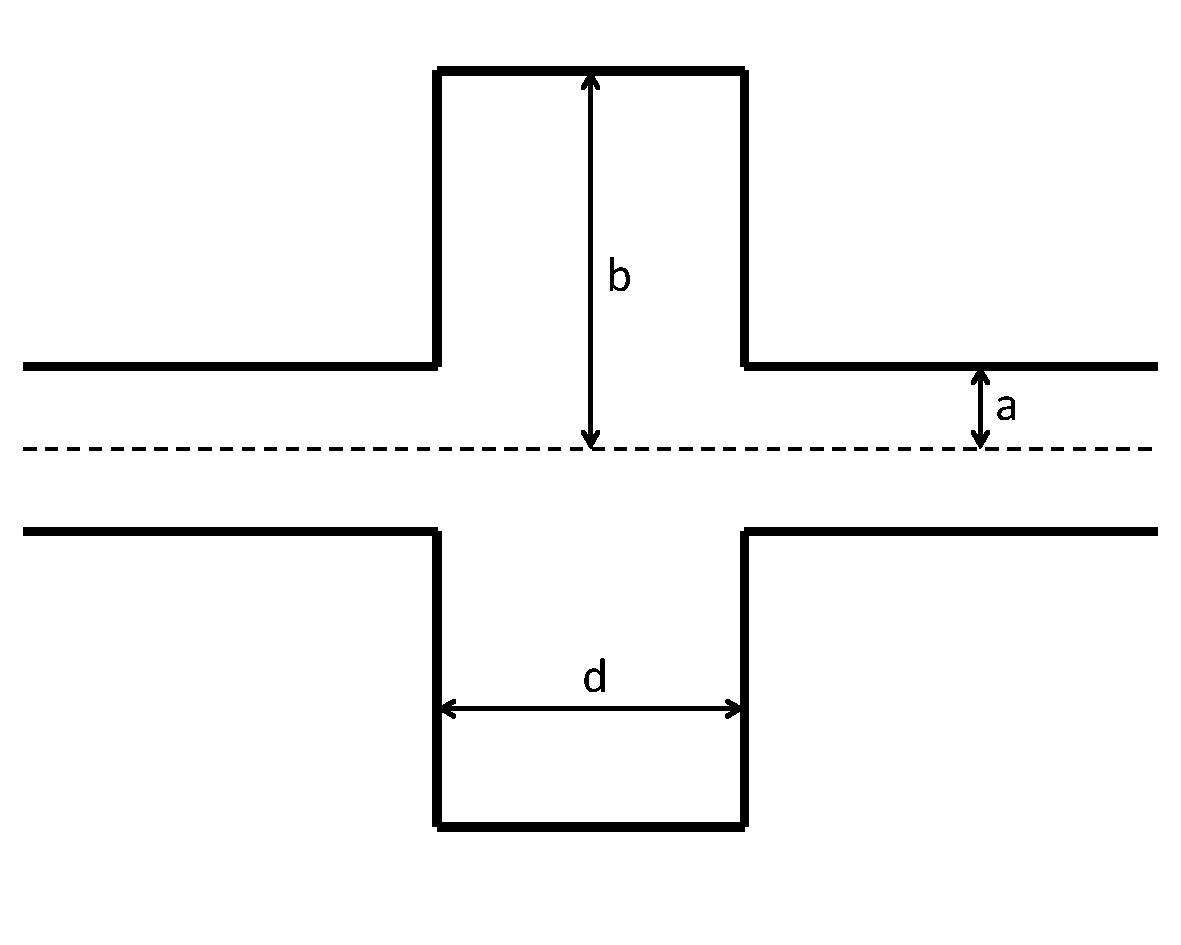
\includegraphics[width=0.5\linewidth]{figures/cavity_beampipe.pdf}
\label{fig:cavity_beampipe}
}
\subfigure[]{
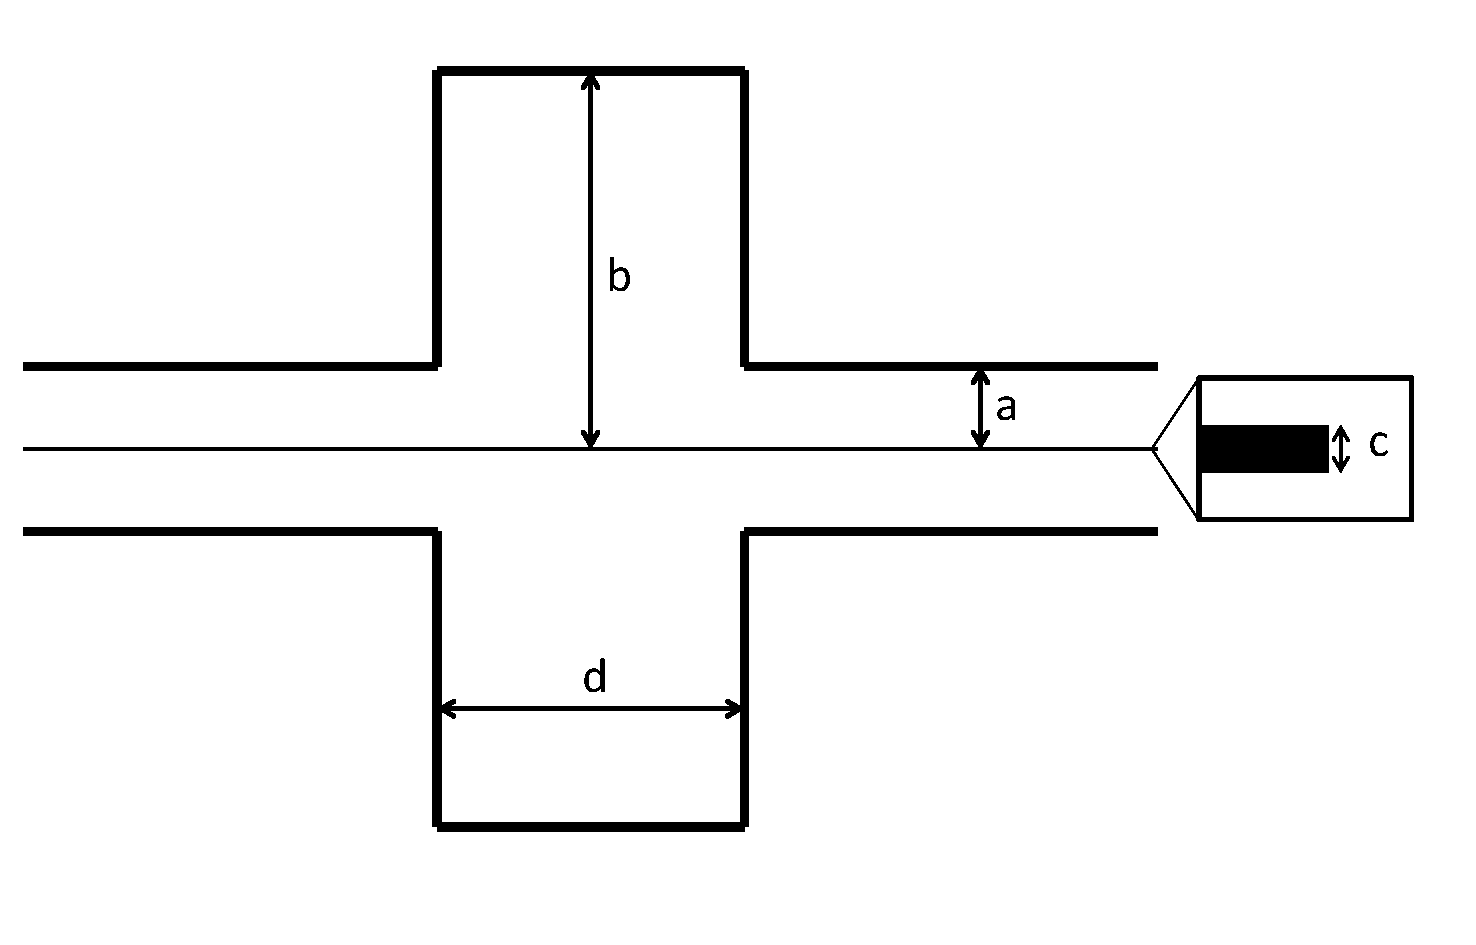
\includegraphics[width=0.625\linewidth]{figures/cavity_beampipe_coaxial.pdf}
\label{fig:cavity_beampipe_coaxial}
}
\caption{Comparison of the geometries of a cavity and attached beampipes \ref{fig:cavity_beampipe} without and \ref{fig:cavity_beampipe_coaxial} with the coaxial wire in place. Note the dimensions and that the dashed line in \ref{fig:cavity_beampipe} represents the rotational plane of symmetry}

\end{figure}

%
%  Things to do for high Q factor measurements
% - Simulation of transmission coefficients with and without coaxial wire
% - Comparison of impedance due to these resonances with time domain simulations
%
%
%
%
%
%
%
%
%
%


%%%%%% Simulations of Beam Impedance %%%%%%%

\chapter{Computational Simulations of Beam Coupling Impedance}
Whilst beam-based measurements and bench-top measurements techniques have been used for some time to measure the impedance of devices and machines, the use of numerical codes to solve 2D and 3D structures is relatively young as a method of identifying the impedance of devices. Recent progress in computational power has now made these a powerful tool in the regime of impedance evaluation. Codes exist that solve simple 2D structures (ECHO2D, ABCI [ref both]), 3D structures (CST Particle Studio, HFSS, Maxwell 3D, ECHO3D, MAFIA) and 3D structures using highly parallelised codes (GdFidl, ACE3P) which allow the simulation of large, complex structures. The codes may be seperated in to two seperate families of codes; time-domain, which calculate the EM fields in a structure by solving Maxwell's equations in the time domain due to a signal inpulse, and frequency-domain which can be used in a number of ways to simulate the beam coupling impedance.

Each of these families of codes has there own relative advantages and disadvantages and peculiarities to use. In this chapter there will a general introduction to a number of the techniques that may be used to calculate the beam coupling impedance from both time-domain and frequency-domain simulations, along with the limitations of each method.
\section{Time Domain Simulations}



\begin{itemize}
\item{A VERY general introduction to time domain simulations codes. This is not a thesis of computational methods, only one thing you may do with them. Write this way}
\item{General experience - advantages of time domain methods (speed, memory footprint). Weaknesses (mesh resolution of structure, CPU limitation, long simulations times for high-Q resonances)}
\end{itemize}

\subsection{Direct Simulation of a Particle Beam}

A large majority of time domain simulation codes (ECHO, MAFIA, CST Particle Studio, GdfidL) use a method that in effect simulates the passage of a particle beam through the structure and evaluates the subsequent electromagnetic fields in the structure by this signal. This is done in the following way:

\begin{enumerate}
\item{A signal representing the source bunch is defined using a given profile, and then passed through the structure from a defined starting displacement and at a given velocity. Additionally a line of integration is defined along which the witness signal will be taken. This is effect defines a source bunch and a witness particle.}
\item{The simulation is propogated for a given period of time to acquire a significant quantity of the wakefield to correctly analyse the frequency components. It can be seen that for both high-Q resonances and low frequencies this requires a longer wakelength, to encompass the long damping time and correctly resolve the signal this frequency respectively.}
\item{The observed signal is subsequently deconvolved with the source signal to obtain a single particle wakefunction.}
\item{This may then be fourier transformed (using an FFT algorithm or other numerical methods) to acquire the beam coupling impedance.}
\end{enumerate}

These steps are illustrated for clarity in Fig.~\ref{fig:time_domain_beam} using a simple pillbox cavity as an example using the time domain code CST Particle Studio.

\begin{figure}
\subfigure[]{

\label{fig:cst_source_signal}
}
\subfigure[]{

\label{fig:cst_witness_signal}
}
\subfigure[]{

\label{fig:cst_wakepotential}
}
\subfigure[]{

\label{fig:cst_impedance}
}

\caption{An illusration of the \ref{fig:cst_source_signal} source signal and \ref{fig:cst_witness_signal} witness integration in a time domain code. The source signal and the resulting wakefield are shown in \ref{fig:cst_wakepotential}, and the subsequent calculated impedance in \ref{fig:cst_impedance}.}
\ref{fig:time_domain_beam}
\end{figure}

It can readily be seen that by defining either the source signal or witness at different displacements it is possible to acquire both the dipolar and quadrupolar impedances. Additional, by taking the gradient of the transverse impedances any constant transverse impedance terms can also calculated.

\section{Frequency Domain Simulations}

There are a number

\begin{itemize}
\item{Advantages of frequency domain - good resolution of structure by meshing, fast solution for individual modes, accurate for resonant structures. Weaknesses - Very memory intensive. Very time consuming to characterise structures over a large frequency ranges}
\end{itemize}

\subsection{Eigenmode Simulations}

Eigenmode solvers are a subset of frequency domain solver that are used to identify strongly resonant modes in a structure. These can be cavity modes, antenna like oscillations or a number of other resonances within the structure. The resulting output of the simulation is typically the resonant frequency of the eigenmode(s), the quality factor $Q$ of the mode (if lossy boundary materials are defined) and the field pattern of the eigenmode solution.

From the field pattern it is possible to readily calculate the longitudinal and transverse $R/Q$ of each cavity mode as defined in Sec.~\ref{sec:sec:imp_geo_imp}. The field patterns may also be used to calculate a number of other properties for each eigenmode, such as surface losses and stored energy in the cavity, which will be explained in further details in Sec.~\ref{sec:ferrite_damping}.

\begin{itemize}
\item{To identify cavity modes of structures}
\item{Extract the resonant frequency and Q of cavity modes}
\item{fields on axis/off axis to extract R/Q, transverse R/Q}
\end{itemize}

\subsection{The Coaxial Wire Method by Simulation}

The coaxial wire method as described in Sec.~\ref{sec:coax_wire_meth} can be directly simulated using waveguide ports to represent matched connections at the ends of the device under test. The resulting simulations provide a transmission coefficient $S_{21}$ which may subsequently be evaluated in the same manner as measurements made with a physical wire. As with the measurements used in practice, a displaced wire and two wires may be simulated and again treated as measurements.

\begin{itemize}
\item{port solutions for driven modal simulations}
\item{Allow the extraction of S21}
\item{Evaluate as in previous section}
\end{itemize}

\subsection{Simulation of the particle beam}

It is also possible to simulate a particle beam directly in the frequency domain. This is done by defining a wave source that produces a field similar to that of the particle beam. For ultrarelativistic beams this neccessitates a source field that is tangential to the direction of motion, and this may technically be possible for cases in which $\beta < 1$. The field components due to the source may be acquired and are the equivalent of the wakefield contribution at a given frequency. The beam impedance $Z$ can subsequently be easily evaluated from the resulting fields

\begin{itemize}
\item{Refer back to the nature of the EM field surrounding a charged particle beam (TEM-like)}
\item{We can enforce a TEM like profile on emitted radiation of a surface}
\item{With a TEM source with no wire - basically a particle beam}
\item{Evaluation as mentioned in Oleksey's paper}
\end{itemize}

%%%%%% Beam Impedance Reduction Techniques %%%%%

\chapter{Beam Coupling Impedance Reduction Techniques}
\begin{itemize}
\item{Introduction to the concepts behind impedance reduction - we must let the image currents follow a path of miniml resistance}
\item{Commence introduction to different impedance reduction methods}
\end{itemize}
\section{Tapering of Step Transitions}
\label{sec:step_ins}

Although the ideal beam pipe of an accelerator would be a pipe of unchanging diameter, it is often necessary to vary the width of the beam pipe for the use of beam instrumentation, insertion devices and machine protection, amongst others. As was shown in Sec.~\ref{sec:imp_geo_imp}, the presence of changes in the pipe diameters gives rise to beam impedance originating at the point of transition. It has been previously demonstrated that this impedance is heavily influenced by the angle of the transition [cite], in addition to the frequency of the resonance of the resulting cavity structure. In particular, this has an influence on the low-frequency broadband impedance, with gentler slopes causing a reduction in the low-frequency impedance. 

There are of course space constraints which restrict the length which tapers may have, both in terms of machine length and the neccessities of size due to the correct operation of the device (for example, collimators or beam instrumentation such as synchrotron radiation monitors). And example of this approach is shown in Fig.~\ref{fig:taper_ex}. This reduction technique has a strong effect of the broadband impedance contribution of a strong resonant impedance caused by step transitions. In particular, it is effective at reducing the imaginary component of the longitudinal beam coupling impedance, as could be seen in the design of the LHC Yellow Book design report for instance [cite]. In this case it was determined that all transitions must observe a maximum gradient of 15$^{\circ}$ unless a design requirement neccessitated otherwise.

\begin{figure}
\subfigure[]{

\label{fig:taper_geometry}
}
\subfigure[]{

\label{fig:taper_impedance}
}

\label{fig:taper_ex}
\caption{An example pillbox structure with and without a tapered transition region \ref{fig:taper_geometry}, in this case with the taper at 45$^{\circ}$. The resulting imaginary component of the longitudinal impedances are shown in \ref{fig:taper_impedance}, as these are the most significant for beam stability.}
\end{figure}

\begin{itemize}
\item{Introduction to the changes in impedance with the steepness of a taper}
\end{itemize}
\section{Transition Pieces}
\label{sec:transitions}

Often it is necessary to have transitions in the beam pipe which can not be tapered, either due to space constraints or the operational requirements of the device containing the transition. This a common requirement in devices that require some mechanical freedom, such as bellows, or electrical isolation from the beam pipe, such as kicker magnets. For these devices it is often possible to use a transition piece, that is a one or several pieces of conducting material to screen any transition. These may be rigid, as is shown in Fig.~\ref{fig:transition_pieces}, or moveable as shown in Fig.~\ref{fig:rf_fingers}, often referred to as RF fingers.

\begin{figure}
\subfigure[]{

\label{fig:transition_pieces}
}
\subfigure[]{

\label{fig:rf_fingers}
}

\label{fig:transition_pieces_geo}
\caption{Examples of both \ref{fig:transition_pieces} transition pieces (for the SPS Injection Kicker Magnets, between the kicker cells and the vacuum tank) and \ref{fig:rf_fingers} RF fingers (in this case for the PIMS module, placed between cryo-modules in the LHC).}
\end{figure}


This method of impedance reduction is effective for a number of reasons. Firstly it provides a short, good conducting path for the image currents to flow that does not expose it to the cavity created by the transition. This serves to reduce the broadband impedance increase due to the transition. Secondly, by correctly designing the spacing in the transitions, it is possible to minimise field leakage to the surrounding cavities therefore decreasing the visibility of cavity resonances. As an example of a cavity with and without RF fingers and a number of intermediatary steps, see Fig.~\ref{fig:rf_finger_imp}, which illustrates the case of the VMTSA, a vacuum interconnect in the injection region of the LHC. It is characterised by a large vacuum chamber (due to needing to contain two circulating beams) with a long set of bellows. They were screened by a long set of RF fingers, which functioned well when good surface contact was maintained between the fingers and the beam pipe. However, when this connection was disrupted (easily created via mechanical stress due to the weak pressure exerted by the afixing spring).


\begin{figure}
\subfigure[]{

\label{fig:vmtsa_operations}
}
\subfigure[]{

\label{fig:vmtsa_failure}
}

\subfigure[]{

\label{fig:vmtsa_impedance}
}


\label{fig:rf_finger_imp}
\caption{The layout of the RF fingers in the VMTSA both in \ref{fig:vmtsa_operations} the fully operational configuration and \ref{fig:vmtsa_failure} when the RF fingers lose contact. \ref{fig:vmtsa_impedance} shows the resulting beam coupling impedance of the two types of impedance as acquired by coaxial wire measurements.}
\end{figure}
\section{Conductive Coatings}
\label{sec:conductive_coatings}

As can be seen in Sec.~\ref{sec:res_wall_imp}, a higher conductivity in the material seen by the beam in a particle accelerator results a lower beam coupling impedance. Typically this rule of thumb is followed in the design of particle accelerators, however the operational requirements of devices in the machine often require that they not be made from a good conducting material. Examples of this include collimators (requiring high strength, mechanical stability and certain radiation properties),  beam instrumentation and numerous other devices.

It has been seen [citey mccite cite] that a thin layer of high conductivity material placed on the surface of a poorly conducting material can effectively screen the beam from interacting with the poorly conducting material for a large frequency range. This can be explained by considering the skin depth of a material $\delta$. As shown in Sec.~\ref{sec:res_wall_imp}, 

\begin{equation}
\delta \left( \omega \right) = \sqrt{\frac{2}{\mu_{0} \sigma \omega}}.
\end{equation}

The skin depth can be thought of as the distance of penetration of the electromagnetic field into the material. In thus be seen that for a good conducting material like copper ($\sigma_{cu} \approx 6 \times 10^{7} S m^{-1}$), for frequencies of the order of a hundred megahurtz or above, a thickness of a $10\mu m$ is much larger than the skin depth at 100MHz ($\delta \left( 100\text{MHz} \right) = 6\mu m$), thus effectively screening the layer below. For many machines the part of the frequency spectrum of concern is above this area (most electron machines, small hadron colliders). It is possible to use thicker coatings (on the order of millimetres) for machines that require a very broad frequency range screened. This is investigated in detail in Sec.~\ref{sec:phase_2_res_wall}.


\section{Beam screens in kicker magnets}
\label{sec:beam_screens}

A substantial contributor to the beam coupling impedance in many machines, in both the longitudinal and transverse planes, are kicker magnets. These are magnets that generate a pulsed magnetic field for a limited period of time (i.e. not always on during beam operation as the dipoles and quadrupoles used for beam optics are), often for orbit corrections, extraction and injection. They have been known to be a problematic component of particle accelerators for a number of decades, mostly in lepton machines due to the traditionally higher beam currents that operate in these machines.

In lepton machines they suffered from problems of heating due to eddy currents induced by traversing bunches, and the neccessity that a remedy to this solution maintain the rapid rise time of the magnetic field required for normal kicker magnet operation, which typically requires a field rise time on the order of the bunch or bunch train seperation in a machine [citing all the cite]. 

A plain ceramic chamber contributes it's own problem from a beam impedance point of view, especially contributing a large imaginary component to the longitudinal impedance due to it's high permitivitty and poor conductivity. In addition it is liable to build up static charges due to being an insulator in a region subject to high electric and magnetic fields. The solution to these problems neccessitates a thin conductive coating on the inside surface of the chamber, either a continuous thin layer (which itself can greatly reduce the field rise time of the kicker magnetic field), or the use of longitudinal stripes, which carry a large proportion of the beam image current, whilst maintaining the rise time characteristics of the magnetic field.

This method will be studied in further depth in Sec.~\ref{sec:mki_studies}, with particular attention to the limitations in use in a high current hadron machine.

\begin{itemize}
\item{Kickers are usually constructed from materials with either large losses (magnetic losses - ferrite) or from strong segmentations (laminated kickers) - both bad for impedance}
\item{We need kickers - find a way to screen the beam from kicker material whilst allowing the kicker to operate as intended - capacitively coupled screens etc.}
\end{itemize}

\section{Seriagraphy on Kicker Magnets}
\label{sec:seriagraphy}

As described in Sec.~\ref{sec:beam_screens}, kicker magnets are often a substantial contributor towards beam coupling impedance. For many machines they were not foreseen to be a limiting factor to beam operation during construction due to either low beam current, long bunch lengths, large bunch seperations or both. However, with increasing improvements in machine performance, it is possible that they may become a limiting factor, as was the case in the SPS extraction kicker magnets[cite]. 

For these existing devices, limitations of both time and budget may require the use of retroactive solutions to large beam impedances. Often these must be added to the original equipment, as the continued correct operation of the device requires minimal disruption to the geometry and surfaces of the device. In the case of the SPS extraction kicker magnet (SPS-MKE), the aperture size had to be preserved, as well as the field rise time of the kicker. In this an innovative solution was found - The use of seriagraphy. This entailed the printing of a set of interleaved fingers (see Fig.~\ref{fig:mke_figures}) made from a good conductor (in the case of the SPS-MKE silver), which form a good conductive path for the beam image currents, capactively coupled across the seperation of the interleaved fingers. This serves to replace the broadband impedance typically associated with a ferrite dominated resistive wall impedance with a low broadband impedance, with strong resonant impedances due to the capcitively coupling and physical length of the fingers. The results in the case of the SPS-MKE can be seen in Fig.~\ref{fig:mke_impedance}.


\begin{figure}
\subfigure[]{

\label{fig:mke_layout}
}
\subfigure[]{

\label{fig:mke_picture}
}
\subfigure[]{

\label{fig:mke_impedance}
}

\caption{An example of seriagraphy in the SPS Extraction Kicker Magnets (SPS-MKE). The layout of the interleaved fingers is shown in \ref{fig:mke_layout} and the actual seriagraphed magnets in \ref{fig:mke_picture}. A comparison of the longitudinal beam coupling impedance with and without the seriagraphy is shown in \ref{fig:mke_impedance}.}
\label{fig:mke_figures}
\end{figure}

\begin{itemize}
\item{Kicker magnet problems, introduced in }

\end{itemize}
\section{Use of damping materials to de-Q resonant caviities}
\label{sec:damping_materials}

For a number of devices it is unavoidable to have a cavity present in the structure. In addition it is often not possible to design the cavity with either tapering or transition pieces due to the need for moveable components, such as a wire scanner or a collimator whose aperture changes with beam parameters. In this case it is necessary to find a way of reducing the beam impedance by altering the properties of resonances. Often it is only the peak value of the impedance attributable to a resonance that is of concern from a beam stability/beam induced heating point of view. 

If we consider the defining properties of a resonant impedance, $f_{res}$, $R/Q$ and $Q$, there are a number of properties that should be noted in changing them. Both $f_{res}$ and $R/Q$ are strongly determined by the geometry of the structure, and thus can not be significantly modified without possibly neccessitating a modification of the device being altered which may hinder the intended operation. Thus one approach to use is to alter the Q of the resonance. A well known method of altering the Q of a resonant cavity is to add a dispersive or ferritic material to the cavity volume [cite ferrite RF cavities from CAS RF for accelerators], that is a material that has complex permitivitty or permeability , given by $\epsilon_{r} = \epsilon^{'} - j \epsilon^{''}$ and $\mu_{r} = \mu^{'} - j \mu^{''}$ respectively. An example of the permeability of some sample ferrite damping materials is shown in Fig.~\ref{fig:ferr_mu_damp}

\begin{figure}

\label{fig:ferr_mu_damp}
\caption{The complex permeability of a number of sample materials used to damp cavity modes.}
\end{figure}

The addition of this family of materials to the cavity has the following effect on the cavity resonances:

\begin{enumerate}
\item{The resonant frequency of any resonance $\omega_{res}$ is reduced by the inclusion of the dispersive material. This can be understood either by considering the $\mu_{r} / \epsilon_{r}$ increasing the effective electrical volume of the cavity by it's inclusion, thereby increasing the dimensions of the resonant cavity. Alternatively, considering the RLC equivalent circuit of a cavity resonance, the inclusion of the dispersive material increases either or both of (depending the properties of the material) the inductance and capacitance of the cavity.}
\item{The $R/Q$ of the cavity experiences little change. There is a slight modification; either an increase that can be attributed to the increased stored energy in the cavity mode due to $\epsilon^{'} \> 1$ or a decrease due to the reaaranging field patterns (caused by the incluson of the dispersive material) decreasing the stored energy.}
\item{The $Q$ of the resonance is drastically reduced. This is due to the strong change in the damping time of the resonance that the addition of the damping material. In terms of cavity properties this can be thought of as the losses in the cavity increasing more rapidly than the stored energy in the cavity. In equivalent circuit terms this may be thought of as the capacitance of the cavity decreasing or the inductance increasing depending on whether a dielectric or ferrous material is added.}
\end{enumerate} 

As can be seen, the resulting effect is to drastically reduce the $Q$ of a cavity resonance, and then by the relation $R_{s} = R_{s}/Q Q$ it can be seen that the shunt impedance will decrease proportional to $Q$. This reduces the peak of $R_{s}$, but broadens the width of the resonance peak, as can be seen in Fig.~\ref{fig:shunt_imp_q_change}. This indicates two effects of using damping materials as an impedance reduction technique; effects dependent on the shunt impedance $R_{s}$ are suppressed, however effects dependent on the broadband behaviour may suffer negatively as a result. Due to the strong frequency dependent nature of many impedance-driven instability mechanisms and beam-induced heating, these negative side effects rarely outway the benefits using damping material in a cavity if necessary.


\begin{figure}

\label{fig:shunt_imp_q_change}
\caption{The change in the peak impedance value of a cavity impedance with a constant R/Q, but changing Q.}
\end{figure}

\subsection{Heat Loads on the Damping Material}

During experience of estimating the heat loads on ferrite damped cavities in high intensity hadron machines (see Sec.~\ref{sec:tctp} for more details), a number of surprising observations were made. In particular was that the placement of ferrite in a cavity does not always produce a significant reduction in the $Q$ of a resonance and that is such cases the percentage of the power loss in the ferrite was comparatively small compared to conventional wisdom, this being that the ferrite experienced the majority of the heat load of the damped cavity. It was thus decided to investigate how the addition of a damping material, in this case a ferrous material, to a cavity would alter both the characteristic resonance properties of the cavity and the location of the power load due to interaction with the beam in the cavity.

Two different geometries were used, one of which could be treated analytically to provide a benchmark for the simulation code, and one in which the ferrite is shielded from being directly seen by the traversing beam, as is normally done to reduce the effects of a resistive wall type impedance due to the ferrite. These geometries are shown in Fig.~\ref{fig:ferr_cav_res}. A single eigenmode of each cavity is investigated, both with and without a damping material. 

\begin{figure}
\subfigure[]{
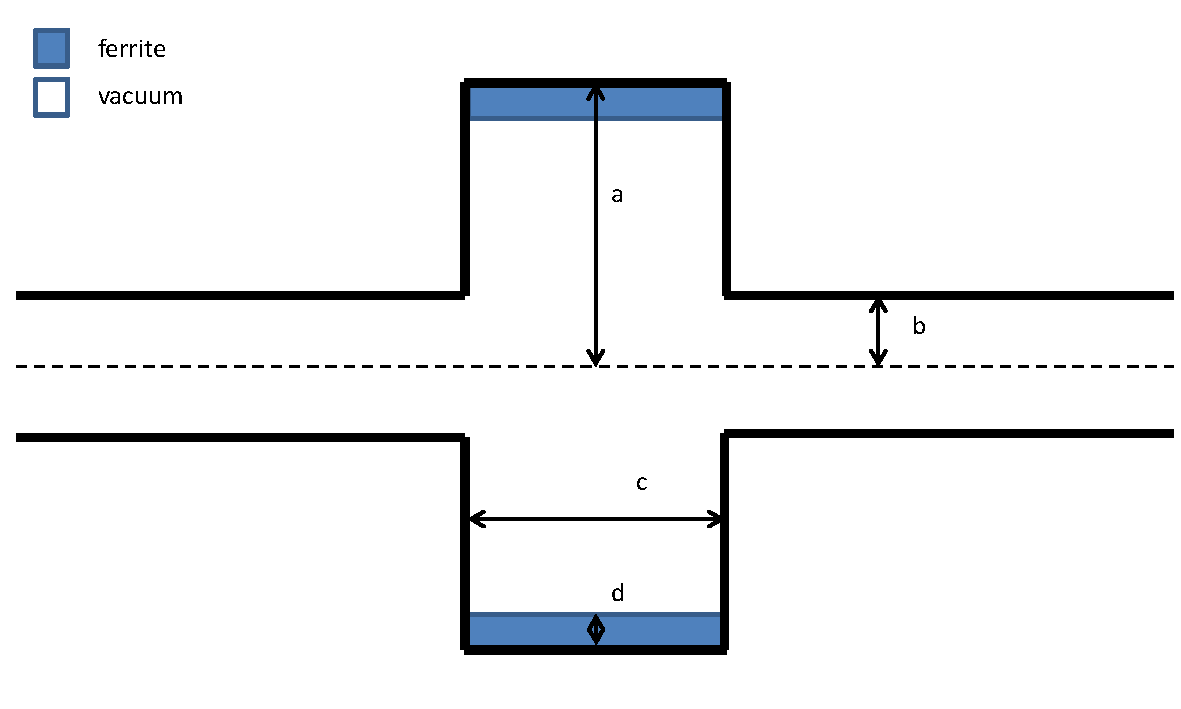
\includegraphics[width=0.45\textwidth]{Beam_Coupling_Impedance_Reduction_Techniques/figures/pillbox_cavity_ferr.pdf}
\label{fig:cav_ferr_no_shield}
}
\subfigure[]{
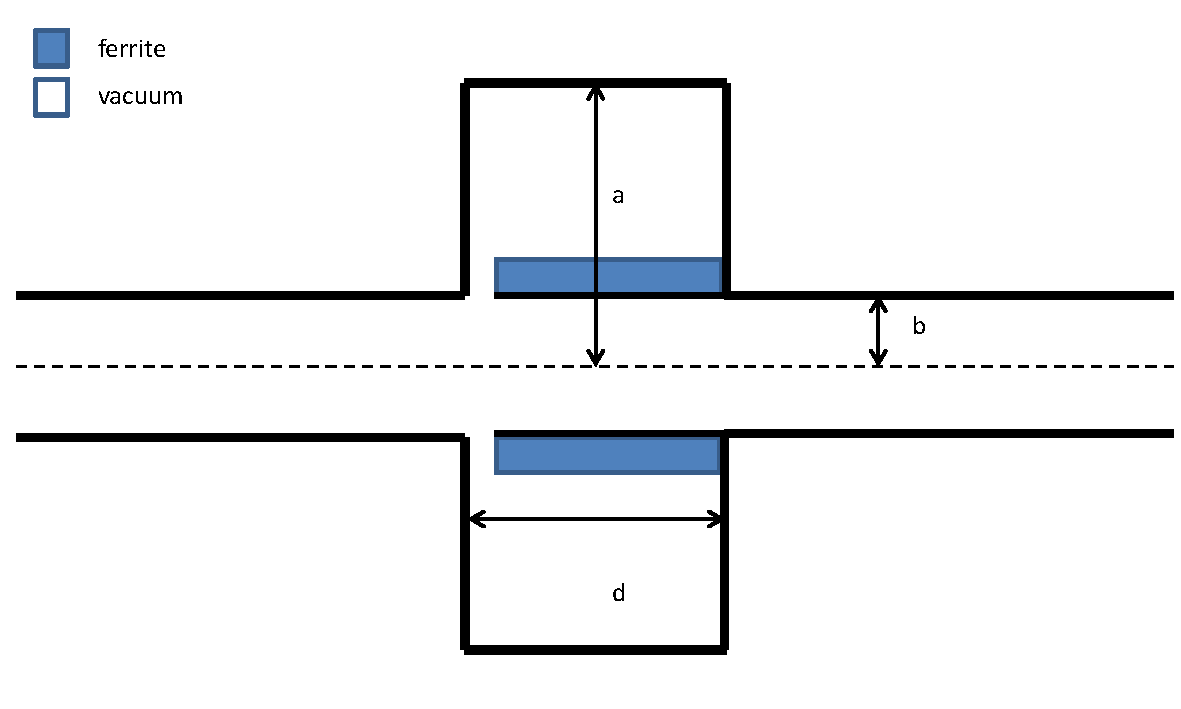
\includegraphics[width=0.45\textwidth]{Beam_Coupling_Impedance_Reduction_Techniques/figures/pillbox_cavity_shielded_ferr.pdf}
\label{fig:cav_ferr_shield}
}
\label{fig:ferr_cav_res}
\caption{Two sample geometries used to examine the effects of ferrite damping material on cavity resonances. \ref{fig:cav_ferr_no_shield} shows a cavity with the ferrite unshielded, and \ref{fig:cav_ferr_shield} shows a more realistic case in which the ferrite is shielded from directly seeing the traversing beam.}
\end{figure}

For this analysis, a cavity of dimensions $a=60mm$, $b=5mm$, $c=20mm$, made from a material with a conductivity $\sigma = 1.1 \times 10^{6} S m^{-1}$ is used for the simulations of an unshielded cavity. A layer of "ferrite" 0.5mm thick is placed as shown in Fig~\ref{fig:cav_ferr_no_shield}. This material is given the following properties: $\epsilon^{'} = 10$, $\epsilon^{''}/\epsilon^{'} = 0$, $\mu^{'}=/1$. $\mu^{''}/ \mu^{'}$ is changed between 0 and 0.02 in steps of 0.02 in order to alter the Q of the resonant mode in incremental steps with the intent of observing how the properties of the cavity change with different scales of damping of the resonance. The "ferrite" is also given a mild conductivity ($\sigma_{ferr} = 10^{-6} S m^{-1}$) as is normal in accelerator ferrites to reduce electrostatic charge build up. For comparison to an analytical formalism, we use the Biancacci finite length impedance model for axisymmetric structures [cite Biancacci IPAC '12].

For the shielded geometry, we use a cavity of the same dimensions as for the unshielded case, with a layer of conductive material 1mm thick placed on the interior of the cavity. A gap of 5mm is left between the beam pipe and the cavity for the beam to couple to the cavity. A ring of ferrite 0.5mm in thickness is then placed on this surface as is shown in Fig.~\ref{fig:cav_ferr_shield}.

Before carrying out the analysis of the location of the heat loss in ferrite, it is prudent verify that the losses calculated using the field calculator in HFSS are self-consistent and well understood. HFSS calculates two losses internally; the surface loss density and volume loss density. The surface loss density $p_{s}$ is defined in HFSS as

\begin{equation}
p_{s} = \Re{}e \left( \mathbf{S}.\mathbf{n} \right)
\end{equation}

where $\mathbf{S}$ is the Poynting vector and $n$ is the out normal vector to the surface boundary[cite HFSS docs]. By integrating this over all surfaces the total surface losses in the cavity are obtained. The total wall losses are also given by 

\begin{equation}
P_{loss, wall} = \frac{R_{wall}}{2} \int_{S} \left| \mathbf{H_{surf}} \right|^{2} dS
\label{eqn:wall_losses}
\end{equation}

where $R_{wall}$ is the surface resistance of the wall and $\mathbf{H_{surf}}$ is the surface magnetic field.

HFSS defines the volume loss density $p_{v}$ as 

\begin{equation}
p_{v}=\frac{1}{2}\Re{}e\left( \mathbf{E}.\mathbf{J} + \left( -\mathbf{\nabla} \times \mathbf{E} \right).\mathbf{H} \right) 
\label{eqn:vol_loss_density}
\end{equation}

where again this may be intergrated over all space to obtain the total volume losses. In addition to these methods of loss calculations of the losses due to the fields in the cavity, it is possible to calculate an equivalent loss of a particle traversing on axis. By considerations of ohmic losses, with the voltage $V$ that experienced by the particle traversing the cavity, the voltage $R = R_{s}$ the shunt impedance of the cavity resonance and $I$ the beam current. As the eigenmode simulation does not directly simulate a beam, the effective power loss is given by 

\begin{equation}
P_{loss} = \frac{V^{2}}{R_{s}}.
\end{equation}

The surface losses and volume losses are subsequently seperately compared. For the surface losses, the internal surface loss density integrated over all surfaces calculated by HFSS, wall losses as given by Eqn.~\ref{fig:wall_losses} and the equivalent losses of a particle on axis are compared. For this we use the unscreened cavity with no ferrite present to have only surface losses present. The different calculated results are shown in Tab.~\ref{tab:surface_losses_ferr}, given in watts normalised to a peak electric field of $1v m^{-1}$ in the cavity. It can be seen that the two calculations due to the surface fields themselves agree exceptionally well, and the calculation for the equivalent loss of an on-axis particle is agrees to within 20\%. 

\begin{table}
\caption{Comparison of the power loss on the surface of a pillbox cavity by both direct calculation and internal calculation by HFSS (In units normalised to 1V/m maximum electric field)}
\begin{center}
\begin{tabular}{c | c }
Calculation Type & Normalised Power Loss (W)\\ \hline
Direct Calculation & 6.2e-10\\ \hline
HFSS Internal Loss Calculations & 6.22e-10 \\ \hline
Loss of an on-axis particle	 & 5.1e-10 \\
\end{tabular}
\end{center}
\label{tab:surface_losses_ferr}
\end{table}

For the volume losses the cavity geometry for the unshielded case is used, with a layer of ferrite 0.5mm thick on inside surface of the cavity. This ferrite has the following material properties; $\epsilon^{'} = 10$, $\epsilon^{'}=0$, $\mu^{'}=10$, $\mu^{"} / \mu^{"} = 0.1$. For this comparison the internal volume loss density integrated over the whole volume as calculated by HFSS, calculating the volume losses using Eqn.~\ref{eqn:vol_loss_density} and the equivalent loss of an on axis particle are calculated, again with loss normalised to a peak electric field of $1 V m^{-1}$ in the cavity. The results are shown in Tab.~\ref{tab:volume_losses_ferr}. It can be seen that the agreement between all three methods of calculating the losses in the cavity is exceptionally good, differing by less than 10\%.

\begin{table}
\caption{Comparison of the power loss in the volume of a pillbox cavity by both direct calculation and internal calculation by HFSS (In units normalised to 1V/m maximum electric field)}
\begin{center}
\begin{tabular}{c | c }
Calculation Type & Normalised Power Loss (W)\\ \hline
Direct Calculation & 1.28e-8\\ \hline
HFSS Internal Loss Calculations & 1.29e-8 \\ \hline
Loss of an on-axis particle & 1.33e-8 \\
\end{tabular}
\end{center}
\label{tab:volume_losses_ferr}
\end{table}


The resulting real component of the longitudinal beam coupling impedance for the case of unshielded ferrite is shown in Fig.~\ref{fig:no_screen_long_imp}. The change in the resonant frequency and the increase in the peak impedancefrom the cavity without any damping material to that with is due to the presence of a region of $\epsilon_{r}>1$. Clearly seen can be the effect of the presence of increasing loss tangent of the ferrite, greatly broadening the impedance peak, with the effect of reducing $R_{s}$ of the resonance. The cause of this reduction of $R_{s}$ can be attributed to the reduction in $Q$ for each resonance, as shown in Fig.~\ref{fig:cav_ferr_no_shield_tan_v_q}. It can be clearly seen that the presence of a small piece of ferrite very strongly decreases the Q of a resonance. The corresponding change in the percentage of the power loss in the ferrite itself as the Q is decreased is shown in Fig.~\ref{fig:cav_ferr_no_shield_q_v_loss_ferr}. It can be seen that the power loss is rapidly localised to the ferrite as the Q decreases. To quantification to this power loss, the power loss due to this cavity resonance is calculated assuming a beam with $1.15 \times 10^{11}$ particles per bunch, 288 bunches, a ring circumference 6911m and a bunch length $4\sigma = 0.04m$ assuming a gaussian bunch distribution and that the resonance falls on a beam harmonic, shown in Fig.~\ref{fig:no_screen_loss_tan_v_power}. Here it can be clearly seen that the power loss in the ferrite rapidly converges to the total losses in the cavity, confirming the assumption that most of the power loss for a cavity resonance damped by a damping material is lost in the damping material. Further information on the numerical results of these simulations is give in Appendix.~\ref{app:ferr_losses}.

\begin{figure}
\begin{center}
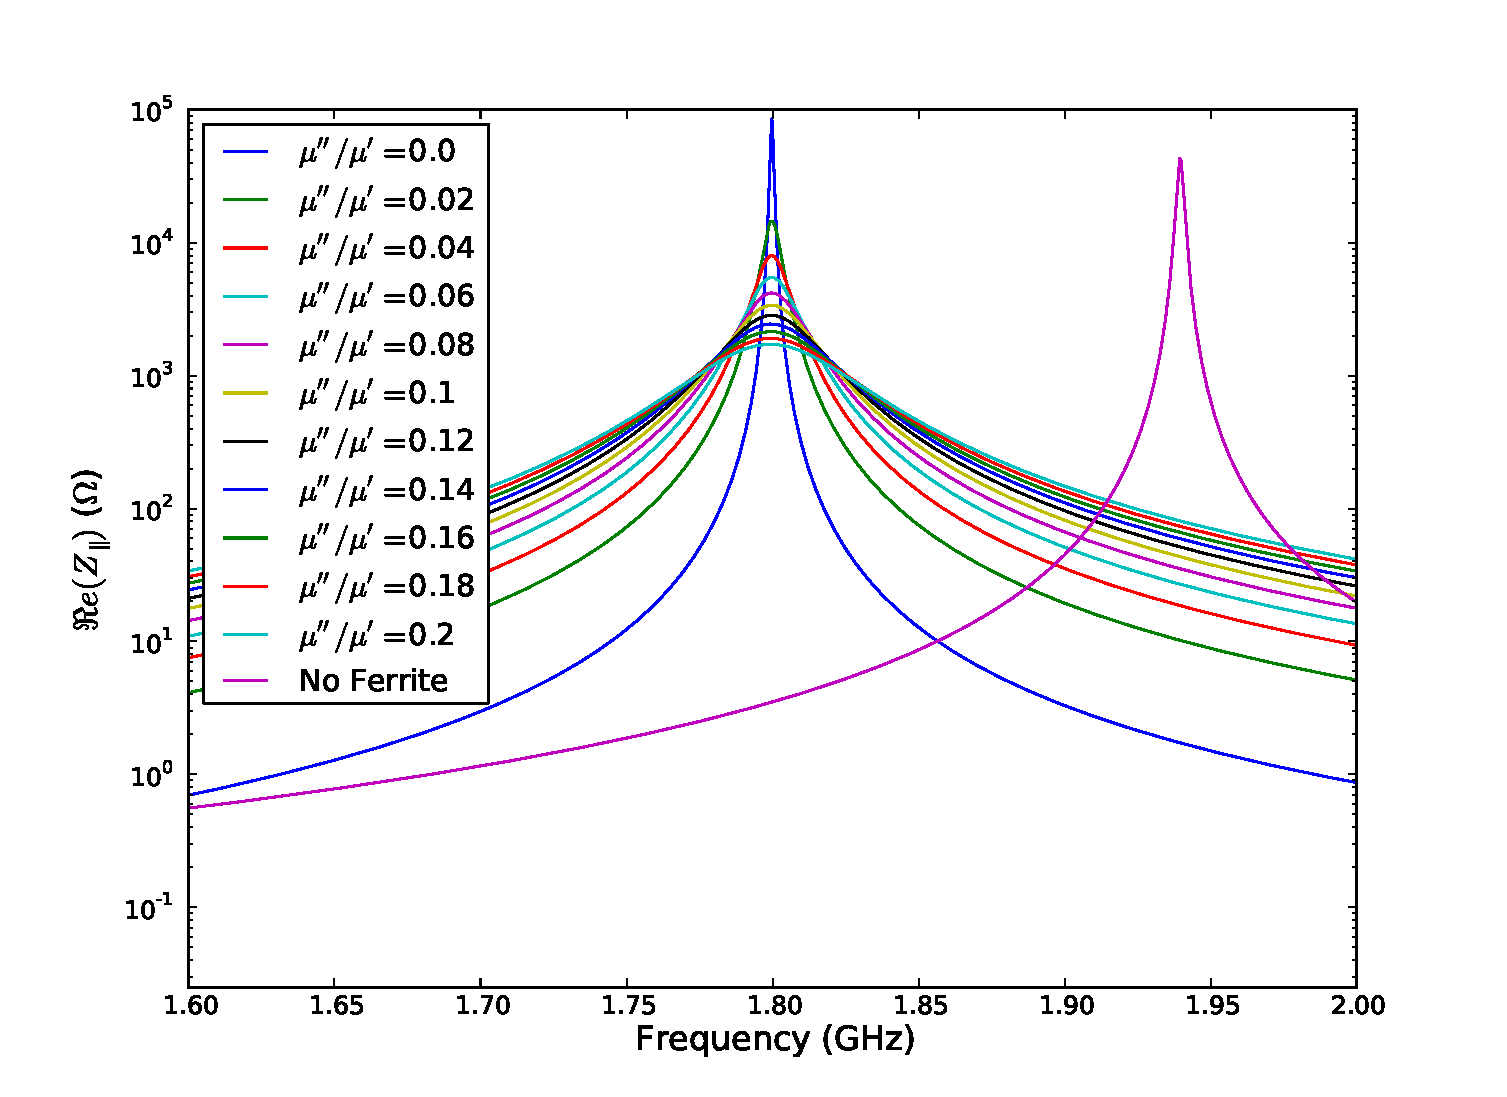
\includegraphics[width=0.7\textwidth]{Beam_Coupling_Impedance_Reduction_Techniques/figures/no_screen_long_imp_all.pdf}
\end{center}
\label{fig:no_screen_long_imp}
\caption{The real component of the longitudinal beam coupling impedance of a cavity without and with a damping material with $\epsilon^{'}=10$, $\mu^{'}=10$ and $\mu^{'}/\mu^{'}$ is varied. The non-damped cavity is shown for comparison. The change in resonance frequency and shunt impedance impedance is due to the increased $\epsilon^{'}$ of the damping material.}
\end{figure}

\begin{figure}
\subfigure[]{
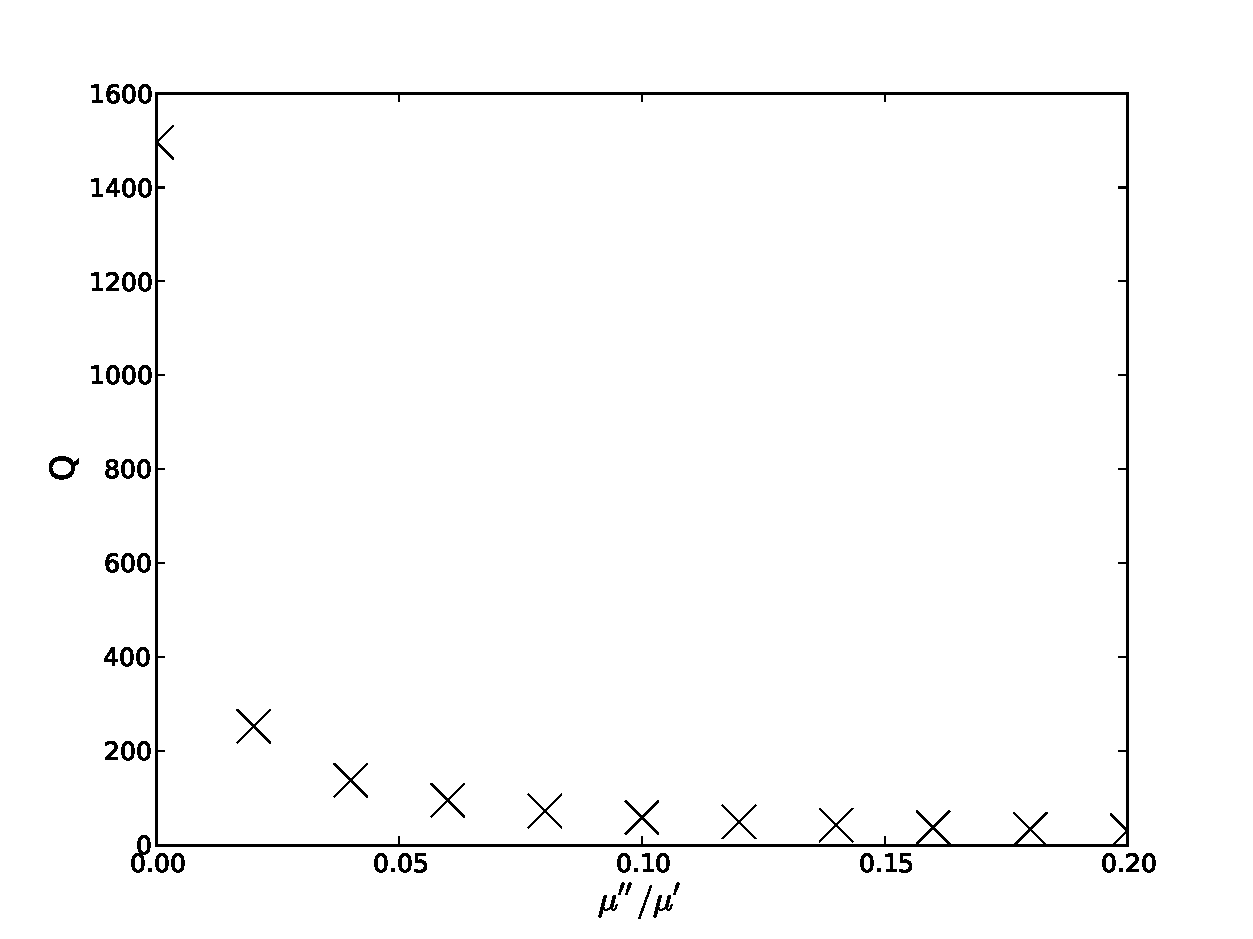
\includegraphics[width=0.45\textwidth]{Beam_Coupling_Impedance_Reduction_Techniques/figures/no_screen_loss_tan_vs_q.pdf}
\label{fig:cav_ferr_no_shield_tan_v_q}
}
\subfigure[]{
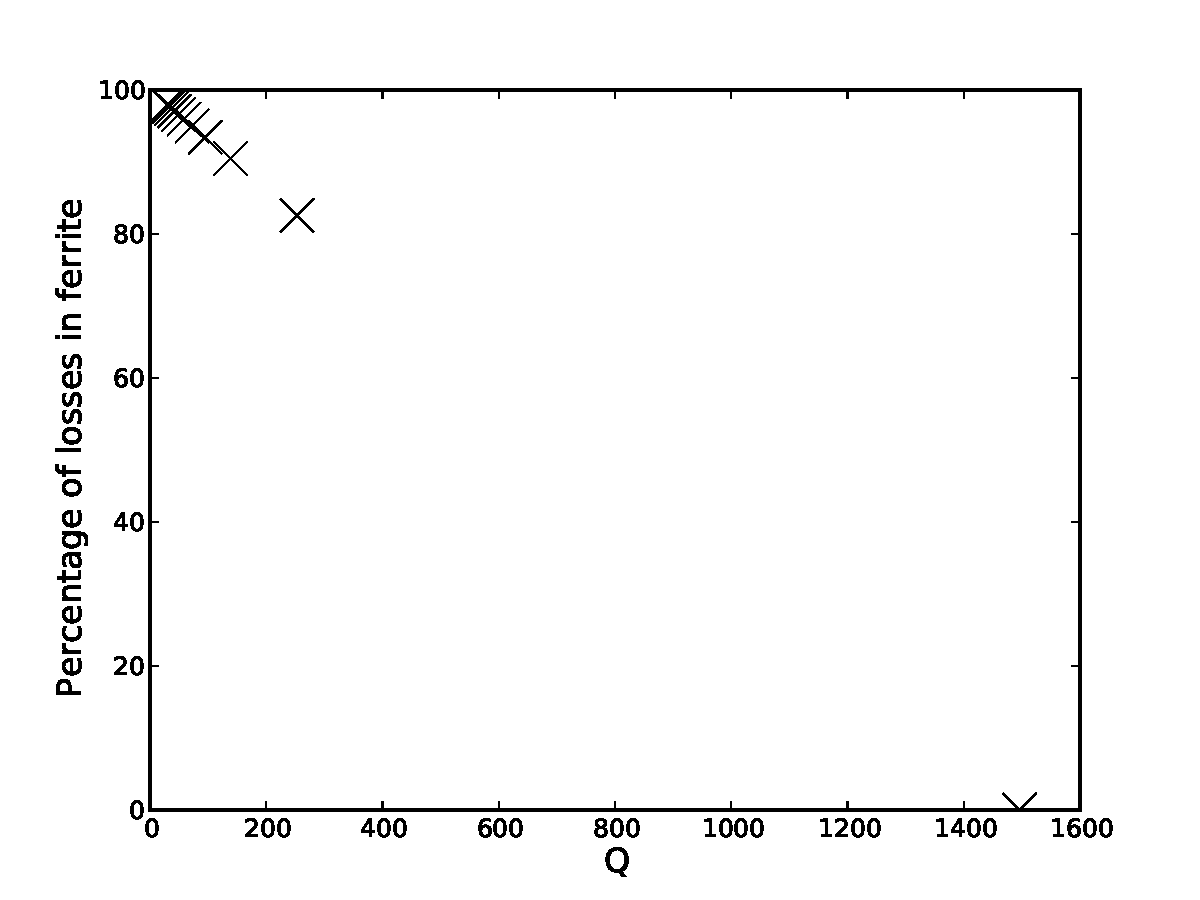
\includegraphics[width=0.45\textwidth]{Beam_Coupling_Impedance_Reduction_Techniques/figures/no_screen_q_vs_loss_ferr.pdf}
\label{fig:cav_ferr_no_shield_q_v_loss_ferr}
}
\label{fig:no_screen_res_alterations}
\caption{\ref{fig:cav_ferr_no_shield_tan_v_q} The reduction in the Q of the cavity resonance with the increasing loss tangent of the ferrite damping, showing a strong decrease of the resonant Q with a small increase in loss tangent. \ref{fig:cav_ferr_no_shield_q_v_loss_ferr} The percentage of the power loss in the ferrite as the resonant Q decreases. this can be seen to tend towards 100\% as the Q approaches 0.}
\end{figure}

\begin{figure}
\begin{center}
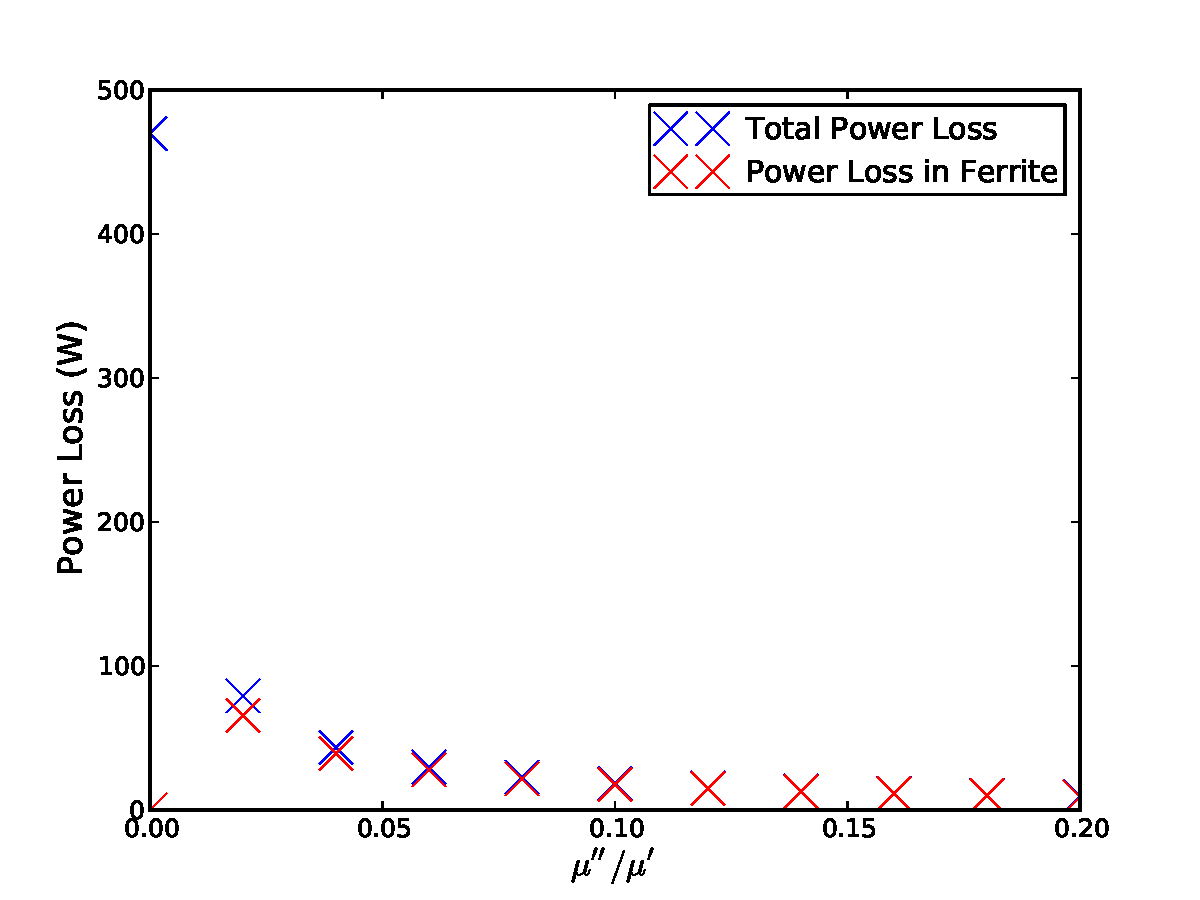
\includegraphics[width=0.7\textwidth]{Beam_Coupling_Impedance_Reduction_Techniques/figures/no_screen_loss_tan_vs_power.pdf}
\end{center}
\label{fig:no_screen_loss_tan_v_power}
\caption{The power loss due to  a beam with $1.15 \times 10^{11}$ particles per bunch, 288 bunches, a ring circumference 6911m and a bunch length $4\sigma = 0.04m$ assuming a gaussian bunch distribution in the unscreened cavity.}
\end{figure}

For the case of the shielded ferrite, the real component of the beam coupling impedance is shown in Fig.~\ref{fig:screen_long_imp}. As with the case of the unshielded ferrite, the addition of the damping material causes a decrease in the resonant frequency of the cavity mode, again due to the addition of a material with $\epsilon_{r} > 1$. In addition, the shielding causes a further decrease in the resonant frequency, in this case due to the rearrangement of the field lines due to the changed boundary conditions.

As can be seen from Fig.~\ref{fig:cav_ferr_shield_tan_v_q} the decrease in the Q of the resonance by the increasing more lossy ferrite follows a similar pattern to that shown by the unshielded structure, as is the increase in the percentage of power loss in the ferrite for the increasing damping of the resonance, shown in Fig.~\ref{fig:cav_ferr_shield_q_v_loss_ferr}. The corresponding change in the power loss in both the cavity as a whole and the ferrite is shown in Fig.~\ref{fig:screen_loss_tan_v_power}. As with the unscreened case, the power lost in the ferrite rapidly converges with the power loss in the entire cavity, indicating that magnetic losses are dominating the losses.	

\begin{figure}
\begin{center}
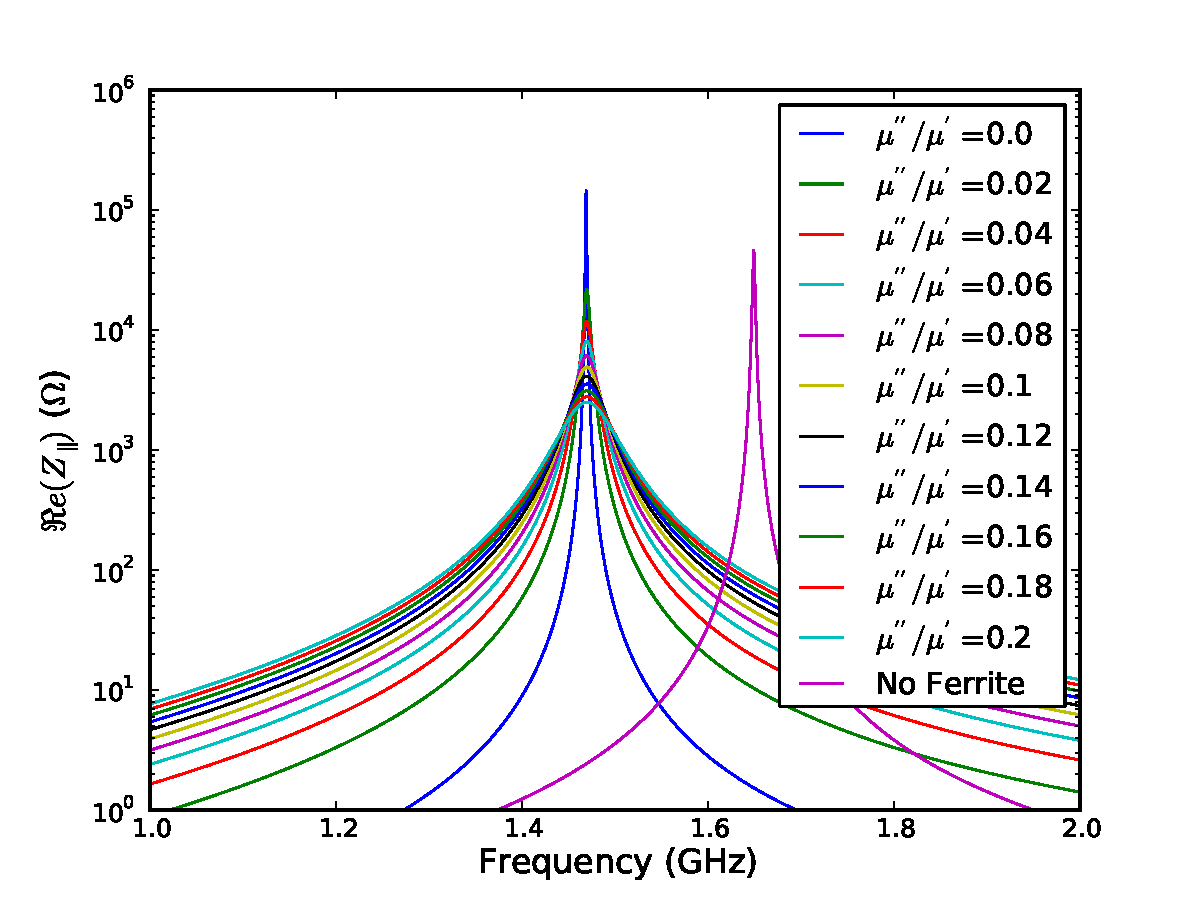
\includegraphics[width=0.7\textwidth]{Beam_Coupling_Impedance_Reduction_Techniques/figures/screen_long_imp_all.pdf}
\end{center}
\label{fig:screen_long_imp}
\caption{The real component of the longitudinal beam coupling impedance of a cavity without and with shielded damping material with $\epsilon^{'}=10$, $\mu^{'}=10$ and $\mu^{'}/\mu^{'}$ is varied. The non-damped cavity is shown for comparison. The change in resonance frequency and shunt impedance impedance is due to the increased $\epsilon^{'}$ of the damping material.}
\end{figure}


\begin{figure}
\subfigure[]{
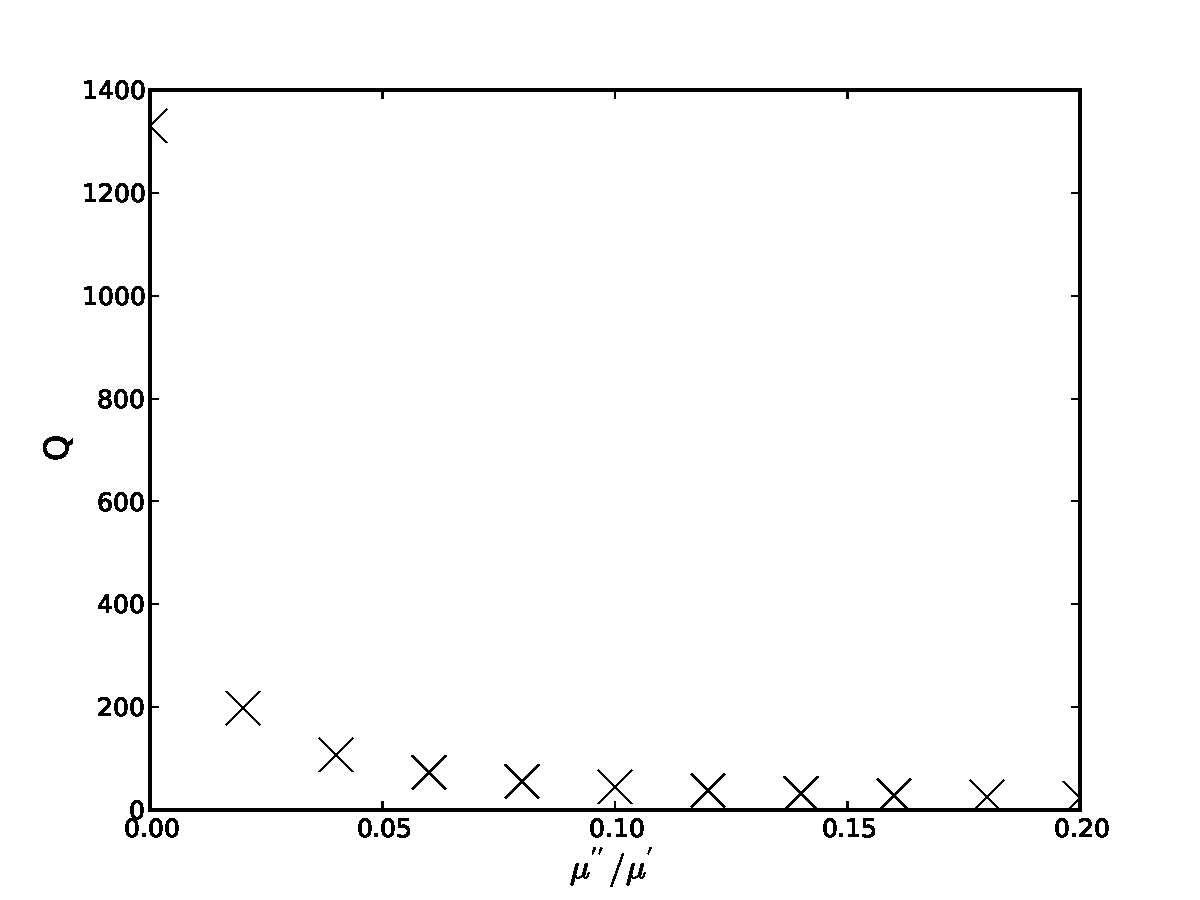
\includegraphics[width=0.45\textwidth]{Beam_Coupling_Impedance_Reduction_Techniques/figures/screen_loss_tan_vs_q.pdf}
\label{fig:cav_ferr_shield_tan_v_q}
}
\subfigure[]{
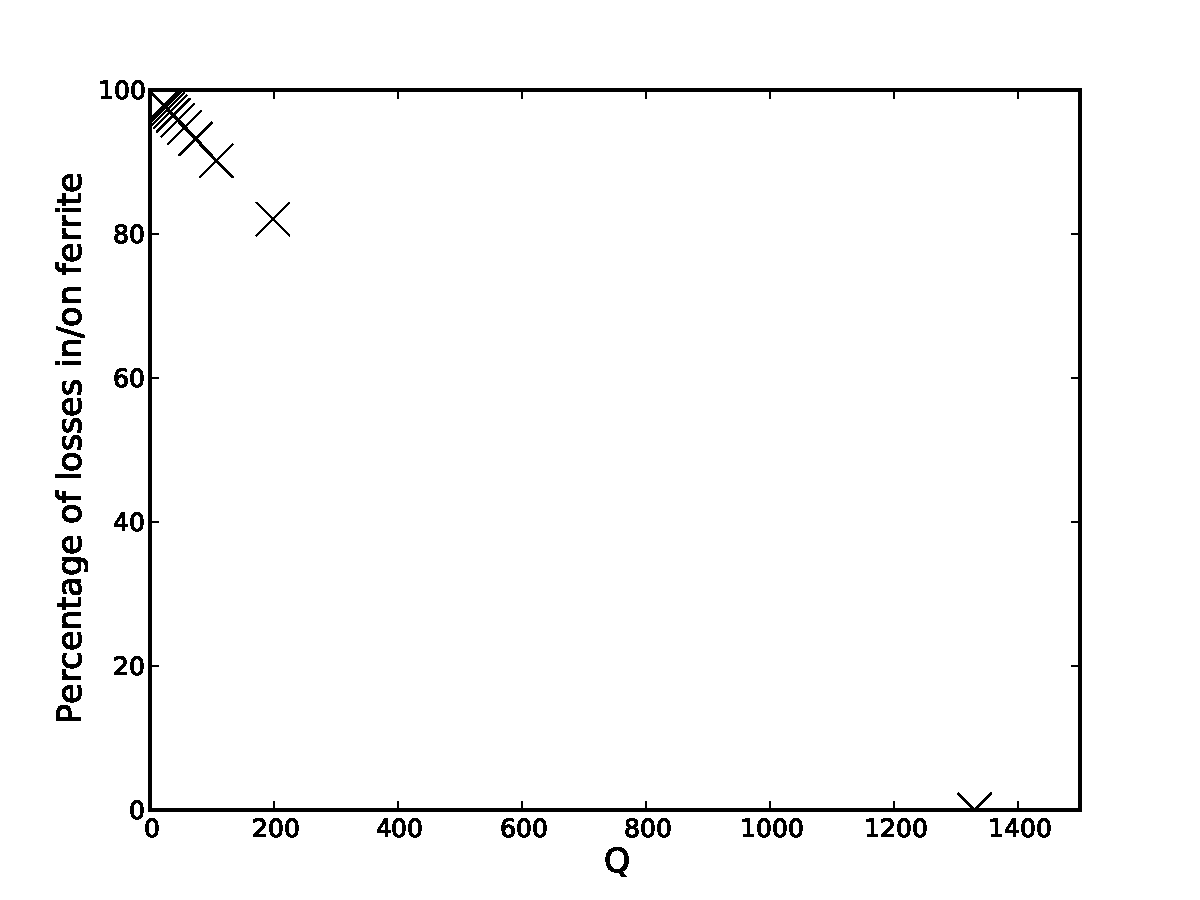
\includegraphics[width=0.45\textwidth]{Beam_Coupling_Impedance_Reduction_Techniques/figures/screen_q_vs_loss_ferr.pdf}
\label{fig:cav_ferr_shield_q_v_loss_ferr}
}
\label{fig:screen_res_alterations}
\caption{\ref{fig:cav_ferr_shield_tan_v_q} The reduction in the Q of the cavity resonance with the increasing loss tangent of the ferrite damping, showing a strong decrease of the resonant Q with a small increase in loss tangent. \ref{fig:cav_ferr_shield_q_v_loss_ferr} The percentage of the power loss in the ferrite as the resonant Q decreases. this can be seen to tend towards 100\% as the Q approaches 0.}
\end{figure}

\begin{figure}
\begin{center}
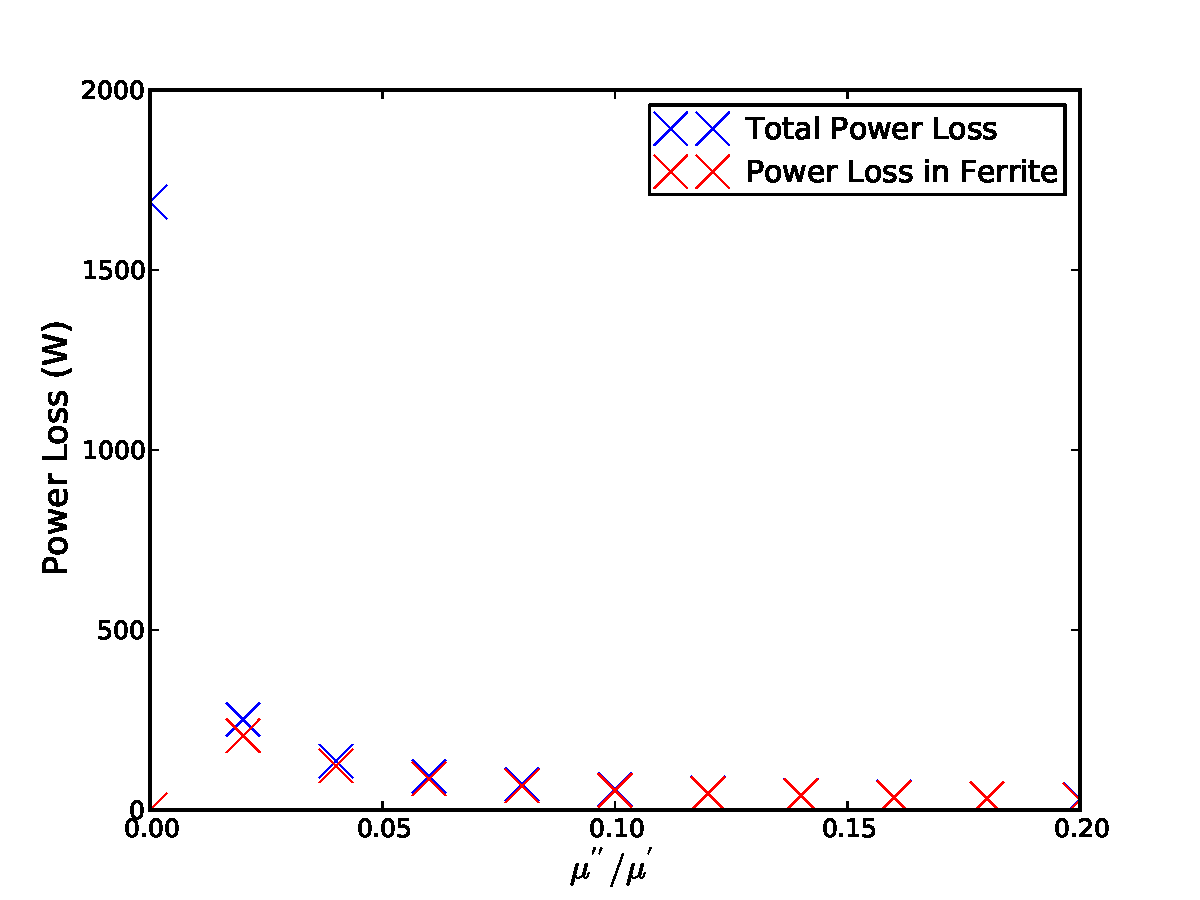
\includegraphics[width=0.7\textwidth]{Beam_Coupling_Impedance_Reduction_Techniques/figures/screen_loss_tan_vs_power.pdf}
\end{center}
\label{fig:screen_loss_tan_v_power}
\caption{The power loss due to a beam with $1.15 \times 10^{11}$ particles per bunch, 288 bunches, a ring circumference 6911m and a bunch length $4\sigma = 0.04m$ assuming a gaussian bunch distribution in the screened cavity.}
\end{figure}

From these results it can thus be seen that the inclusion of the shielding does not substantially effect the losses due to strong cavity resonances, whilst aiding in reducing the effects of image current flowing through the ferrite (a broadband effect, and thus not considered in the eigenmode simulations). In addition, we see that if the cavity mode is strongly damped by the presence of ferrite (i.e. the $Q$ is reduced by a factor 20 or so) it should be expected that the vast majority of the remaining power lost by particles interacting with the cavity resoance should ultimately be lost in the damping material. 

%%%%%% LHC Collimation Upgrades %%%%%%

\chapter{LHC Collimation Upgrades}
\section{Introduction}

The LHC collimation system is a key part of the machine protection system in the LHC. Due to extremely high stored beam and magnetic energy in the LHC [cite], amounting to some 160MJ of beam energy and 3GJ of stored magnetic energy, it is neccessary to keep close control on the losses experienced by the system. In the LHC this is done by a combination of monitoring the losses within the machine, carefully controlled losses by the collimation system, and a rigorous interlock system designed to dump the beam safely in the event of the development of dangerous behaviour by the circulating beam [LHC machine protection].

The collimation system in the LHC is a four-stage system, composed primarily of primary (TCP), secondary (TCS), and tertiary (TCT) collimators. These serve to scatter the particle halo, then further scatter and absorb the scattered particles. Further protection is provided by absorbers (TCLA), collimators at the injection regions (TCLI and TDI) and at the extraction region (TCDQA). In particular the TCTs are placed near the experimental IPs to protect the inner triplet magnets (used for final focusing of the beam before collision). In total the collimation system is broken down into two IRs; IR3 for betatron cleaning, in which there are:

\begin{enumerate}
\item{1 primary collimator}
\item{4 secondary collimators}
\item{4 absorbers}
\end{enumerate}

per beam and IR7 for momentum cleaning, which is composed of:

\begin{enumerate}
\item{3 primary collimators}
\item{11 secondary collimators}
\item{5 absorbers}
\end{enumerate}

per beam, with an additional 8 tertiary collimators (2 per experimental IP) per beam. In addition to the collimators at the injection and extraction region each beam is exposed to 44 different moveable collimators per circulation of the machine. The primary and secondary collimators presently all have a jaw material carbon reinforced graphite (conductivity $\sigma_{graphite} = 7 \times 10^{4} S m^{-1} $). This material was chosen due to the requirement for a robust jaw material (mechanically stable under large thermal shock) from a machine protection point of view, however not optimised from a beam impedance point of view.

The current collimation system has demonstrated to be exceptionally effective at it's job of providing machine protection to the LHC [cite Chamonix 2012 MP presentation], however it has been shown to be a limiting factor in the luminousity of the LHC due to the large contribution to the transverse beam coupling impedance by the primary, and especially the numerous secondary collimators in the system, which are also almost double the length of the primary collimators[cite]. 

\begin{figure}
\subfigure[]{
\label{fig:phase-1-col-longitudinal-rf}
}
\subfigure[]{
\label{fig:phase-1-col-sliding-contacts}
}
\label{fig:pĥase-1-rf}
\caption{Different components the impedance reduction measures in the phase 1 collimator design. \ref{fig:phase-1-col-longitudinal-rf} shows the longitudinal RF fingers, ensuring a good conducting path for the beam image currents, and \ref{fig:phase-1-col-sliding-contacts} shows the sliding RF contacts on the collimators jaw. These are intended to minimise the volume seen by the beam, thus making any cavity modes that may be excited by the beam at very high frequencies where the beam power spectrum is very small.}
\end{figure}

The phase 1 collimator (those presently (as of 2012) in place in the LHC) designs have a number of design features that are designed to reduce the beam coupling impedance of each device. Although the resistive wall contribution to the beam coupling impedance due to the poorly conducting jaw material is significant, the use of longitudinal RF fingers in the transition between the beam pipe to the collimator jaws and of a system of sliding contact fingers to isolate the beam from seeing the collimator vacuum tank (see Fig~\ref{fig:phase-1-rf} for more details). These function well as impedance reduction techniques, however have some limitations from a mechanical point of view. In particular, the sliding contacts have been suspected to be a significant producer of dust in the LHC due to the moving physical contact during collimator alignment [cite]. 

Due to these factors (high transverse impedance due to the resistive wall impedance and problems of dust due to sliding contacts) a phase 2 upgrade of the LHC collimation system has been proposed. This entails two components;

\begin{enumerate}
\item{The replacement of the current secondary collimators (the prime contributor to the large transverse impedance) by a phase 2 design using a good conducting material as the jaw material. There will be some loss of mechnical robustness but it is thought that this will not be detrimental to the requirements of machine protection with a suitable choice of material.}
\item{Replacing the existing sliding RF contacts with a contactless RF system (shown in Fig.~\ref{fig:rf-system-phase-2}). This is designed to remove the problem of dust caused by the sliding RF contacts in the phase 1 system by removing the moving physical contacts. This increase the volume of the cavity visible to the particle beam, decreasing the frequency of the lowest cavity modes. To counteract these new resonances, ferrite is placed in the cavity to decrease the resulting Q of the resonances.}
\end{enumerate}

\begin{figure}
\begin{center}
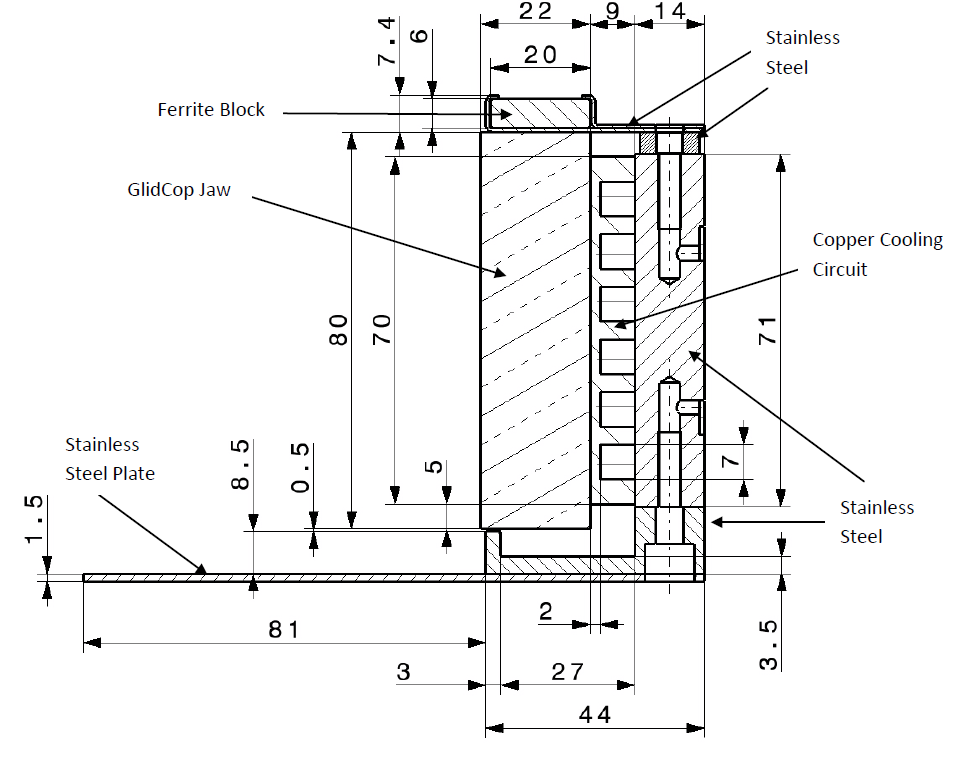
\includegraphics[width=0.7\textwidth]{LHC_Collimation_Upgrades/figures/cu-geo.png}
\end{center}
\label{fig:phase-2-rf-system}
\caption{The RF system for use in the phase 2 collimation system. The sliding RF contacts of the phase 1 design are replaced with a ferrite damping system. The RF contacts are removed, allowing the beam to see the entire RF cavity, causing resonances at lower frequencies. The Q of these resonances are decreased by the use of ferrite damping tiles.}
\end{figure}

In this chapter shall be presented an comparison of the different jaw materials proposed for use in the phase 2 secondary collimators, in particular a combination of jaw materials aimed at combining extremely robust materials with highly conductive metals, and the results of full 3D simulations of a TCTP collimator - a tertiary collimator for use in the LHC - which is incorporates the ferrite damping system in comparison to the sliding contacts of the phase 1 RF system. 



%
% Introduction to the new collimator design - Old collimator design, problems with sliding rails, new design, new material possibilities
% Material Evaluation - Comparison of CST simulations
% Whole collimator simulations of phase 2 secondary - Transverse and longitudinal modes with ferrite - compared to that from phase 1
% Sims in CST PS, GdFidl and HFSS
% Heating calculations also
%
%
%
%
%



\section{LHC Phase 2 Secondary Collimator Jaw Material}

The phase 2 secondary collimators are proposed as an addition to the current phase 1 secondary collimators. They have stringent mechanical requirements, particularly due to the neccessity to withstand impacts by a limited number of bunches in the LHC during injection. In addition they must meet a stringent limit on beam impedance - new devices in the LHC must not increase the total impedance of the machine due to the stability limits imposed due to the existing large transverse and longitudinal impedance. If possible, the effective impedance in the machine should be reduced during operation. 

To meet the strict requirements of the differing physical requirments on the jaw material, both from a mechanical point view and an impedance point of view a number of different jaw design solutions have been proposed. These include both single jaw material designs, mixtures of composites and pure metals, and varities on a design including ceramic. The proposed jaw material combinations are listed below:

\begin{enumerate}
\item{GlidCop, a copper compositie including aluminium oxide particles[ref]. The conductivity is marginally worse than pure copper (see Tab.~\ref{tab:phase2-cond}), but the addition of the aluminium oxide greatly increases the resistance to thermal softening and increases the strength at high temperatures.}
\item{Molybdenum - An metal with good mechanical properties and a conductivity comparable to copper.}
\item{Copper Diamond Composite - A copper composite formed by hot pressing copper with the addition of boron powder and small synthetic diamonds. Produces a very mechanically robust material.}
\item{Molybdenum Diamond Composite - As with the above, a molybdenum compositie formed by the use of sintering molybdenum with artificial diamonds.}
\item{Carbon reinforced carbon (CFC) - The current material of the phase 1 secondary collimators. Included for comparison.}
\end{enumerate}

More information on the material choices can be found in [cite AD/AB papers]. The conductivities of the different materials can be found in Tab.~\ref{tab:phase2-cond}. The layouts of the various possible jaw designs can be found in Fig.~\ref{fig:phase2-jaw-designs}.

\begin{table}
\caption{The electrical conductivity of the different jaw materials proposed for use in the phase 2 design. All results are given for measurements at room temperature (20$^{o}$C)}
\begin{center}
\begin{tabular}{c | c }
Chapter & Completeness \\ \hline
Glidcop & $5.4 \times 10^{7}$ \\ \hline
Molybdenum & $1.87 \times 10^{7}$ \\ \hline
Copper Diamond Compositie (CuCD) & $1.25 \times 10^{7}$ \\ \hline
Molybdenum Diamond Composite (MoCD) & $5.5 \times 10^{6}$ \\ \hline
Graphite & $7 \times 10^{4}$ \\ \hline
\end{tabular}
\end{center}
\label{tab:phase2-cond}
\end{table}

\begin{figure}
\subfigure[]{
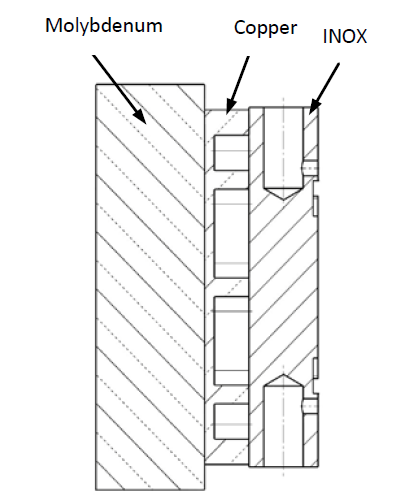
\includegraphics[width=0.45\textwidth]{LHC_Collimation_Upgrades/figures/mo-geo.png}
\label{fig:phase-2-moly}
}
\subfigure[]{
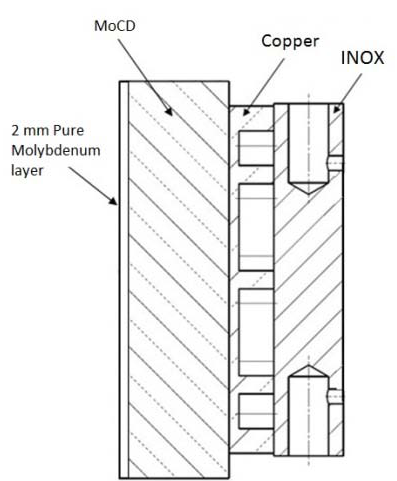
\includegraphics[width=0.45\textwidth]{LHC_Collimation_Upgrades/figures/mo-mocd-geo.png}
\label{fig:phase-2-molycd}
}
\label{fig:phase-2-jaw-designs}
\caption{A number of the proposed jaw designs for the phase 2 secondary collimators. \ref{fig:phase-2-moly} shows the jaw made entirely from molybdenum. Glidcop maybe substituted for molybdenum in this design. \ref{fig:phase-2-molycd} shows the jaw made from a mixture of molybdenum diamond composite with a 2mm coating of molybdenum on the surface. The composite ensure a mechanically strong jaw, whilst the coating screens the higher resistivity composite and provides a smooth surface on the beam-facing part of the jaw. In this case the composite maybe substituted with copper diamond composite, and likewise the coating may be replaced with GlidCop.}
\end{figure}


\begin{itemize}
\item{Introduction to the collimator upgrade project - Why are collimators important}
\begin{enumerate}
\item{The have two significant physical requirements - a rigid, sturdy material and must be placed very close to the beam}
\item{The first necessitated the use of graphite/carbon materials for the phase 1 collimators due to their survivability in the condition needed. The second means that the resistive wall impedance is very large}
\end{enumerate}
\item{Phase 2 collimator materials choice}
\begin{enumerate}
\item{Why a phase 2 collimator upgrade?}
\item{Summary of the material requirements and the available materials}
\item{Simple model used - simulations and comparison to analytical models}
\end{enumerate}

\section{TCTP Impedance Studies}

As part of the ongoing collimation upgrade in the LHC, several advances in the LHC design have been proposed. These are as follows:

\begin{enumerate}
\item{For the reasons given in Sec.~\ref{sec:phase-2-col-mat}, the jaw material of the collimators, specifically the secondary collimators is under review in an effort to reduce the beam impedance, improve cleaning efficiency and continue the present robustness and excellent performance of the LHC collimation system.}
\item{The inclusion of on collimator BPMs. This is due to the present method of alignment of the collimators relying on investigating the beam loss patterns in the LHC as a function of collimator aperture being a very time intensive procedure due to the inherentl slow natyure of beam loss. The use of on collimator BPMs allows a near instantaneous feedback on the position of the beam relative to the collimator jaw thus greatly increasing collimator setup time[cite setup paper gianluca/on collimator BPM paper]}
\item{A new RF system (Shown in Fig.~\ref{fig:phase-2-rf-system}) to reduce the side effects of the sliding RF contacts used in the phase 1 collimators.}
\end{enumerate}

As part of the upgrade, a series of TCTP collimators shall be installed in the LHC in replacement of a number of tertiary collimators (TCTs). In total, 8 TCTP and 1 TCSG will be added to the LHC. These collimators are in part intended to act as a test for two of these upgrades, the use of on collimator BPMs and the new RF system[cite collimators with onboard BPMs]. As part of the ongoing effort to limit increases to the LHC machine impedance (shown in Tab.~\ref{tab:lhc-impedance-budget}) and due to continuing concerns about beam-induced heating [cite cham/evian 2012], all new devices to be placed in the LHC must be examined for their effect on the beam and as a possibly luminuousity limiter in the LHC. Due to the large number of phase 2 secondary collimators that are planned to be put in the LHC (30 additional secondary collimators to be installed during long shutdown 2[cite eucard report]) it is vital that the new collimator design, especially the new RF system is verified for it's efficacy as an impedance reduction technique.  


\begin{table}
\caption{The impedance budgets (both transverse and longitudinal) for LHC. Taken from the LHC Design Report[cite LHC design report 2003-2004]}
\begin{center}
\begin{tabular}{c | c | c}
Beam Operation & Longitudinal $\Im{}m ( Z_{\parallel}/n )$ $( \Omega )$ & Longitudinal $\Im{}m ( Z_{\perp} )$ $( \Omega /m )$\\ \hline
Total Broadband at injection (450GeV) & 0.07 & 1.34 \\ \hline
Total Broadband at collisions with squeezed optics (7TeV) & 0.076 & 2.67 \\ \hline
\end{tabular}
\end{center}
\label{tab:lhc-impedance-budget}
\end{table}


\subsection{TCTP Collimator - Design and Geometry}

The TCTP 
\subsection{Impedance Simulations and Results}
\label{sec:imp-sims-tctp}

The impedance of the TCTP collimator is examined through the use of simulation codes. In order to verify the simulation results it was decided to use both a time domain and a frequency domain code, in this case CST Particle Studio[cite] for the time domain and Ansoft HFSS[cite] for the frequency domain. Due to the reduced simulation time for time domain simulations compared to frequency domain simulations (which must be evaluated mode by mode to correctly evaluate the eigenmodes), the preliminary comparisons are done using the time domain code and the most promising solutions are subsequently investigated in depth using the frequency domain model.

For this comparison we investigate a number of different designs of the RF system for comparison to the ferrite damping solution chosen for construction;

\begin{enumerate}
\item{The phase 1 sliding RF contacts, to provide comparison to the existing RF system. Shown in Fig.~\ref{fig:phase-1-rf}.}
\item{The proposed RF system including the ferrite damping tiles and the RF screen as shown in Fig.~\ref{fig:phase-2-rf-system}.}
\item{The proposed RF system without the ferrite damping tiles. This is too investigate the benefit of including the ferrite tiles.}
\end{enumerate}


\begin{figure}
\subfigure[]{

\label{fig:sliding-contacts}
}
\subfigure[]{

\label{fig:rf-circuit-ferrite}
}
\subfigure[]{

\label{fig:rf-circuit-no-ferrite}
}
\label{fig:rf-systems-tctp}
\caption{The different RF systems considered for the TCTP collimator. \ref{fig:sliding-contacts} shows an RF system similar to the phase 1 RF system. In these simulations the sliding RF contacts are replaced by a perfect connection - for frequencies lower than 2-3GHz this is a good approximation and greatly simplifies the simulation model. \ref{fig:rf-circuit-ferrite} shows the RF circuit complete with ferrite. \ref{fig:rf-circuit-no-ferrite} shows the phase 2 RF circuit but without any ferrite present.}
\end{figure}


The three different systems are shown in Fig.~\ref{fig:rf-systems-tctp}. 



\input{LHC_Collimation_Upgrades/tctp_collimator/transverse_impedance_concerns}
\subsection{Beam-Induced Heating}
\label{sec:beam-heating-tctp}

As seen in Sec.~\ref{sec:imp-sims-tctp}, the longitudinal impedance of the phase 2 RF design indicates a significant number of beam impedance resonances below 1GHz. Although their contribution in the imaginary component of the beam coupling impedance is not significant enough to be of concern from a stability point of view, the resonances may present a problem from the point of view of beam-induced heating. To fully investigate both the effectiveness of the ferrite in damping the cavity resonances and to identify the locations of the power loss the phase 2 structure is investigated using the frequency domain code HFSS. 

For these simulations we simulate half of the structure (due to the reflective symmetry in the longitudinal plane), using alternatively perfect E-field (enforcing perpendicular electric fields at the boundary) and H-field (enforcing perpendicular magnetic fields at the boundary) boundary conditions at the symmetry plane to indentify and characterise the eigenmodes up to 2GHz (to cover the majority of the beam spectrum). The structure with and without ferrite is simulated to characterise the effect of the ferrite in damping the cavity modes. Simulations are carried out using the following parameters:

\begin{itemize}
\item{Using a 2$^{nd}$ order basis function solver to ensure good resolution of the fields for R/Q and localised loss calculations.}
\item{The ferrite is assumed to be 4A4, materials data is imported from an external data file and interpretted fit is used between data points. An analytical model (see [cite entry] for details).}
\item{We simulate using a single jaw seperation, in this case a half-seperation of 2mm. This is an extremely close jaw seperation, closer in fact than the TCTP collimator would be placed at, but similar to that that the phase 2 collimators would be placed at. This allows some prediction of a worst case scenario for the TCTP and also an analysis of the efficacy of the RF system for the type of operational parameters the phase 2 secondary collimators would be placed at.}
\item{The mesh was auto-generated by the HFSS mesh generator, and run for a convergence criteria of a 0.5\% convergence of the eigenmode frequency between two successive meshes with a 30\% refinement of the mesh between successive solutions.}
\end{itemize}

\begin{figure}
\begin{center}
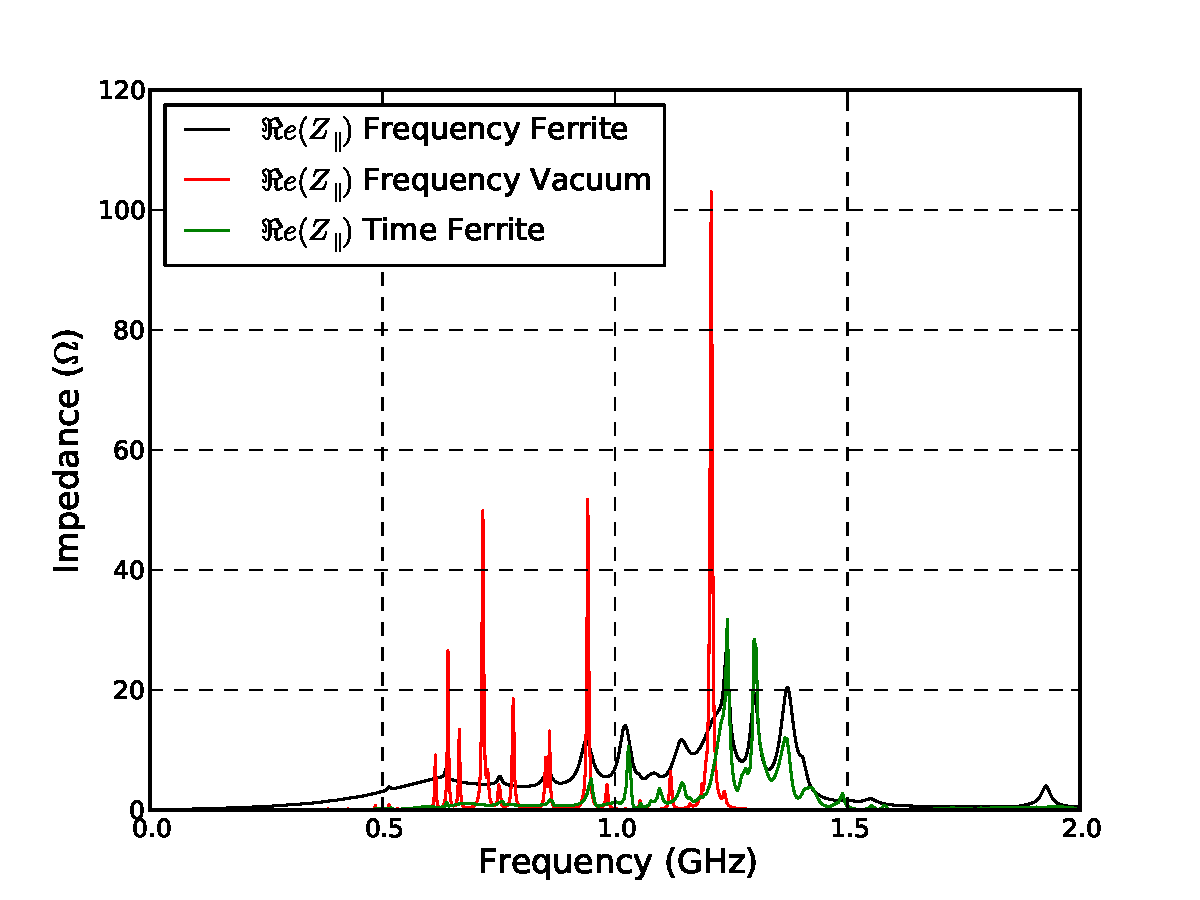
\includegraphics[width=0.7\textwidth]{LHC_Collimation_Upgrades/figures/longitudinal-impedance-tctp-ferr-freq-dom.pdf}
\end{center}
\label{fig:long-imp-tctp-freq}
\caption{The real component of the longitudinal impedance for the TCTP collimator as simulated by both the time and frequency domains for the case with and without ferrite damping tiles. The strong resonances present in the case without ferrite can be seen to be strongly damped when the ferrite tiles are added. However a substantial broadband component occurs in addition due to the broadened resonance peaks.}
\end{figure}

Here we shall evaluate the resonances as a whole, or a few key resonances from a heating point of view. For a complete listing of the eigenmodes please see App.~\ref{app:tctp-eigenmodes} for a complete breakdown of the TCTP eigenmode simulations. To have a comprehensive review of the heating we consider the following heating possibilities

\begin{itemize}
\item{A beam harmonic occuring exactly on the resonant frequency with a certain bunch profile. Here we consider gaussian and cos$^{2}$ bunch profiles. Parameters for a number of different beam operating modes (summarised in Tab.~\ref{tab:lhc-tctp-heating-para}) are considered.}
\item{Taking theoretical spectra for both 50ns and 25ns bunch spacings. In this case we consider the heating for both nominal operational parameters (1ns bunch length), running conditions from 2012 (bunch length between 1.2-1.4ns) and for HL-LHC parameters. These parameters are summarised in Tab.~\ref{tab:lhc-tctp-heating-para}. Different bunch profiles are considered - gaussian and cos$^{2}$ to account for high frequency lobes observed in measured beam spectra.}
\item{Using measured multi-bunch spectra for 50ns bunch spacing measured in the LHC. These measurements are for the beam from injection, through the ramp to squeeze and finally collisions.}
\end{itemize}

\begin{table}
\caption{The LHC operational parameters considered for heating estimates for the TCTP. Operational parameters include the nominal LHC parameters for 25ns bunch spacing, the peak operational intensity for 50ns bunch spacing used in 2012, and the two possible HL-LHC operational schemes, using both 25ns and 50ns bunch spacing. Here the bunch length is assumed to encompass the $4\sigma$ gaussian width.}
\label{tab:lhc-tctp-heating-para}
\begin{center}
\begin{tabular}{c | c | c | c | c }
Operational Mode & $\tau_{b}$ (ns) & $t_{bunch}$ (ns) & $N_{b}$ & $n_{bunches}$ \\ \hline
50ns, 2012 LHC Operation & 1.2 & 50ns & $1.7 \times 10^{11}$ & 1380 \\ \hline
25ns, Nominal LHC Operation & 1.0 & 25ns & $1.15 \times 10^{11}$ & 2808 \\ \hline
HL-LHC 25ns & 1.0 & 25ns & $2.0 \times 10^{11}$ & 2808 \\ \hline
HL-LHC 50ns & 1.0 & 50ns & $3.3 \times 10^{11}$ & 1380 \\ \hline
\end{tabular}
\end{center}
\end{table}

The heating estimates assuming on resonance beam harmonics can be seen in Tab.~\ref{tab:on-res-heating-tctp} for a variety of bunch lengths between 1-1.5ns assuming gaussian and cos$^{2}$ bunch distributions. The same data for the TCTP without the ferrite damping tiles can be seen in Tab.~\ref{tab:on-res-heating-tctp-no-ferr}. A number of things area immediately evident; 	The addition of the ferrite drastically reduces the power loss in the TCTP collimator, by a factor of $\approx$ 3. In addition, the consideration of the higher frequency lobes in the heating estimates for the TCTP is significant, as can be seen in Fig.~\ref{fig:tctp-heating-bunch-length-per-freq}. In this case the usefulness for the ferrites is clear.

\begin{table}
\label{tab:on-res-heating-tctp}
\caption{The power loss of a the TCTP collimator with ferrite for a number of operational modes in the LHC and HL-LHC assuming each cavity mode falls upon a beam harmonic. All losses are in watts using the parameters found in Tab.~\ref{tab:lhc-tctp-heating-para}}
\begin{center}
\begin{tabular}{c | c | c | c | c | c | c | c | c  }
$\tau_{b}$ (ns) & \multicolumn{2}{| c |}{50ns, 2012} & \multicolumn{2}{| c |}{25ns nominal} & \multicolumn{2}{| c |}{50ns, HL-LHC} & \multicolumn{2}{| c }{25ns, HL-LHC} \\ \hline
 & $P_{loss, g}$ & $P_{loss, c}$ & $P_{loss, g}$ & $P_{loss, c}$ & $P_{loss, g}$ & $P_{loss, c}$ & $P_{loss, g}$ & $P_{loss, c}$ \\ \hline
1.0 & 5.6 & 14.2 & 10.6 & 27.0 & 21 & 53.4 & 32.2 & 81.8 \\ \hline
1.1 & 3.8 & 10.2 & 7.2 & 19.6 & 14.4 & 38.8 & 22.0 & 59.0 \\ \hline
1.2 & 2.6 & 7.4 & 5.0 & 14.0 & 10.2 & 27.8 & 15.4 & 42.2 \\ \hline
1.3 & 2.0 & 5.4 & 3.6 & 10.0 & 7.2 & 20.0 & 11.0 & 30.4 \\ \hline
1.4 & 1.4 & 3.8 & 2.6 & 7.4 & 5.2 & 14.6 & 8.0 & 22.2 \\ \hline
1.5 & 1.0 & 2.8 & 2.0 & 5.4 & 3.8 & 10.8 & 5.8 & 16.4 \\ \hline
\end{tabular}
\end{center}
\end{table}

\begin{table}
\label{tab:on-res-heating-tctp-no-ferr}
\caption{The power loss of a TCTP collimator without the ferrite damping tiles for a number of operational modes in the LHC and HL-LHC assuming each cavity mode falls upon a beam harmonic. All losses are in watts using the parameters found in Tab.~\ref{tab:lhc-tctp-heating-para}}
\begin{center}
\begin{tabular}{c | c | c | c | c | c | c | c | c  }
$\tau_{b}$ (ns) & \multicolumn{2}{| c |}{50ns, 2012} & \multicolumn{2}{| c |}{25ns nominal} & \multicolumn{2}{| c |}{50ns, HL-LHC} & \multicolumn{2}{| c }{25ns, HL-LHC} \\ \hline
 & $P_{loss, g}$ & $P_{loss, c}$ & $P_{loss, g}$ & $P_{loss, c}$ & $P_{loss, g}$ & $P_{loss, c}$ & $P_{loss, g}$ & $P_{loss, c}$ \\ \hline
1.0 & 2.8 & 7.1 & 5.3 & 13.5 & 10.5 & 26.7 & 16.1 & 40.9 \\ \hline
1.1 & 1.9 & 5.1 & 3.6 & 9.8 & 7.2 & 19.4 & 11.0 & 29.5 \\ \hline
1.2 & 1.3 & 3.7 & 2.5 & 7.0 & 5.1 & 13.9 & 7.7 & 21.1 \\ \hline
1.3 & 1.0 & 2.7 &1.8 & 5.0 & 3.6 & 10.0 & 5.5 & 15.2 \\ \hline
1.4 & 0.7 & 1.9 & 1.3 & 3.7 &2.6 & 7.3 & 4.0 & 11.1 \\ \hline
1.5 & 0.5 & 1.4 & 1.0 & 2.7 & 1.9 & 5.4 & 2.9 & 8.2 \\ \hline
\end{tabular}
\end{center}
\end{table}

\begin{figure}
\label{fig:tctp-heating-bunch-length-per-freq}
\caption{The beam-induced heating of the TCTP with ferrite damping tiles for a number of different bunch lengths assuming both a gaussian and cos$^{2}$ distributions.}
\end{figure}

Considering the heating taking beam harmonics seperated the inverse of the bunch seperation (40$MHz$ for $t_{bunch} = 25ns$ and 20$MHz$ for $t_{bunch} = 50ns$) we acquire the results presented in Tab.~\ref{tab:heating-beam-harm-tctp-ferr} and Tab.~\ref{tab:heating-beam-harm-tctp-no-ferr} respectively, again for a variety of LHC operational parameters and assuming either a gaussian or a cos$^{2}$ longitudinal bunch profile. In this case it can be seen that the power loss for the ferrite case is larger than that experienced by the case without ferrite. This can be understood due to the fixed frequencies of the beam harmonics - if a high-Q resonance does not occur at or near a beam harmonic then the beam does not couple to the resonance. Due to the broad resonance peaks of the ferrite damped TCTP design the beam may couple to the resonance even if the resonance frequency of the cavity mode does not match the beam harmonic precisely due to the low-Q of the resonance.

\begin{table}
\label{tab:heating-beam-harm-tctp-ferr}
\caption{The power loss of a TCTP collimator with ferrite for a number of operational modes in the LHC and HL-LHC assuming beam harmonics spaced at the reciprocal of the bunch spacing. All losses are in watts using the parameters found in Tab.~\ref{tab:lhc-tctp-heating-para}}
\begin{center}
\begin{tabular}{c | c | c | c | c | c | c | c | c  }
$\tau_{b}$ (ns) & \multicolumn{2}{| c |}{50ns, 2012} & \multicolumn{2}{| c |}{25ns nominal} & \multicolumn{2}{| c |}{50ns, HL-LHC} & \multicolumn{2}{| c }{25ns, HL-LHC} \\ \hline
 & $P_{loss, g}$ & $P_{loss, c}$ & $P_{loss, g}$ & $P_{loss, c}$ & $P_{loss, g}$ & $P_{loss, c}$ & $P_{loss, g}$ & $P_{loss, c}$ \\ \hline
1.0 & 19.0 & 36.2 & 18.2 & 35.0 & 71.6 & 136.8 & 54.8 & 104.6 \\ \hline
1.1 & 14.8 & 29.2 & 14.2 & 28.0 & 56.2 & 110.0 & 42.8 & 85.0 \\ \hline
1.2 & 11.8 & 23.6 & 11.2 & 22.6 & 44.8 & 89 & 34.0 & 68.6 \\ \hline
1.3 & 9.6 & 19.2 & 9.0 & 18.4 & 36.2 & 72.6 & 27.4 & 55.6 \\ \hline
1.4 & 7.8 & 16.0 & 7.4 & 15.2 & 29.4 & 60.0 & 22.2 & 45.8 \\ \hline
1.5 & 6.4 & 13.2 & 6.0 & 12.6 & 24.2 & 50.0 & 18.4 & 38.0 \\ \hline
\end{tabular}
\end{center}
\end{table}

\begin{table}
\label{tab:heating-beam-harm-tctp-no-ferr}
\caption{The power loss of a TCTP collimator without ferrite for a number of operational modes in the LHC and HL-LHC assuming beam harmonics spaced at the reciprocal of the bunch spacing. All losses are in watts using the parameters found in Tab.~\ref{tab:lhc-tctp-heating-para}}
\begin{center}
\begin{tabular}{c | c | c | c | c | c | c | c | c  }
$\tau_{b}$ (ns) & \multicolumn{2}{| c |}{50ns, 2012} & \multicolumn{2}{| c |}{25ns nominal} & \multicolumn{2}{| c |}{50ns, HL-LHC} & \multicolumn{2}{| c }{25ns, HL-LHC} \\ \hline
 & $P_{loss, g}$ & $P_{loss, c}$ & $P_{loss, g}$ & $P_{loss, c}$ & $P_{loss, g}$ & $P_{loss, c}$ & $P_{loss, g}$ & $P_{loss, c}$ \\ \hline
1.0 & 2.8 & 7.1 & 5.3 & 13.5 & 12.1 & 25.0 & 16.1 & 40.9 \\ \hline
1.1 & 1.9 & 5.1 & 3.6 & 9.8 & 7.2 & 19.4 & 11.0 & 29.5 \\ \hline
1.2 & 1.3 & 3.7 & 2.5 & 7.0 & 5.1 & 13.9 & 7.7 & 21.1 \\ \hline
1.3 & 1.0 & 2.7 &1.8 & 5.0 & 3.6 & 10.0 & 5.5 & 15.2 \\ \hline
1.4 & 0.7 & 1.9 & 1.3 & 3.7 &2.6 & 7.3 & 4.0 & 11.1 \\ \hline
1.5 & 0.5 & 1.4 & 1.0 & 2.7 & 1.9 & 5.4 & 2.9 & 8.2 \\ 
\end{tabular}
\end{center}
\end{table}



\subsubsection{Location of Power Deposition}

\begin{figure}
\subfigure[]{

\label{fig:tctp-ferrite}
}
\subfigure[]{

\label{fig:tctp-long-rf-finger}
}

\label{fig:tctp-heat-loc}
\caption{The different thermally sensitive components of the TCTP collimator. \ref{fig:tctp-ferrite} shows the ferrite tiles, and \ref{fig:tctp-long-rf-finger} the longitudinal RF fingers.}
\end{figure}

Due to the poor cooling available in vacuum (cooled by radiative heating only. Although surrounded by a housing/in contact with surrounded components, the thermal contact between different components within the collimator is poor) it is important to know of the proportion of beam-induced power loss that is lost in thermally sensitive areas. These are areas where large increases in temperature can either lead to direct physical damage (as is the case with RF fingers) or may lead to a worsening physical condition of the collimator (if the ferrite tiles go above their Curie temperature). The components are highlighted in Fig.~\ref{fig:tctp-heat-loc}

The losses on or in different surfaces and volumes is calculated using the loss calculations within HFSS, and then normalised to the total losses in the TCTP structure for each mode. The produces a variety of losses depending on the field pattern of the mode. These are collated in App.~\ref{app:tctp-eigenmodes}. To provide a conservative estimate of the power load we take the highest proportions of power loss of all the modes and assume this is the case for all modes. The percentages for the total device, the ferrite tiles and the longitudinal RF fingers are shown in Tab.~\ref{tab:tctp-heating-loc}. 

\begin{table}
\label{tab:tctp-heating-loc}
\caption{The percentage of power loss lost in thermally sensitive components in the TCTP.}
\begin{center}
\begin{tabular}{c | c}
Component & Percentage of Power Loss \\ \hline
Whole Device & 100 \\ \hline
Ferrite Tiles & 5 \\ \hline
Longitudinal RF Fingers & 4 \\
\end{tabular}
\end{center}
\end{table}

\begin{table}
\label{tab:heating-ferr-power-load}
\caption{The power loss in the ferrite of the TCTP collimator. The most pessimistic of the losses estimated in Tab.~\ref{tab:on-res-heating-tctp} and Tab.~\ref{tab:heating-beam-harm-tctp-ferr} for the 1.0ns case. All losses are in watts using the parameters found in Tab.~\ref{tab:lhc-tctp-heating-para}}
\begin{center}
\begin{tabular}{c | c | c | c | c }
$\tau_{b}$ (ns) & 50ns, 2012 & 25ns nominal & 50ns, HL-LHC & 25ns, HL-LHC \\ \hline
 &  $P_{loss, c}$  & $P_{loss, c}$ &  $P_{loss, c}$  & $P_{loss, c}$ \\ \hline
1.0 & 1.8 & 1.7 & 6.8 & 5.2 
\end{tabular}
\end{center}
\end{table}


The thermal behaviour as a result of this power load can be analysed using design software such as ANSYS[cite]. The results of these thermal simulations can be seen in [cite F. Carra/M. Garlasche colwg meeting], a summary of which is given in Fig.~\ref{fig:tctp-ferrite-temp-rise}. The important figure of merit is in whether the temperature of the ferrite increases beyond its Curie temperature. For the TT2-111R, this 375$^{\circ}$C[cite data sheet]. The power loss for the worst cases of the nominal, HL-LHC and HL-LHC parameters without crab cavities (bunch length $0.5$ns rather than $1.0$ns) is considered, in this case with a factor of two margin of error included to be conservative (i.e. we assume double the power on the ferrite tiles), and it can be seen that the temperature increase for even the worst case results in the temperature being significantly below the Curie temperature for this material.

\begin{figure}
\begin{center}
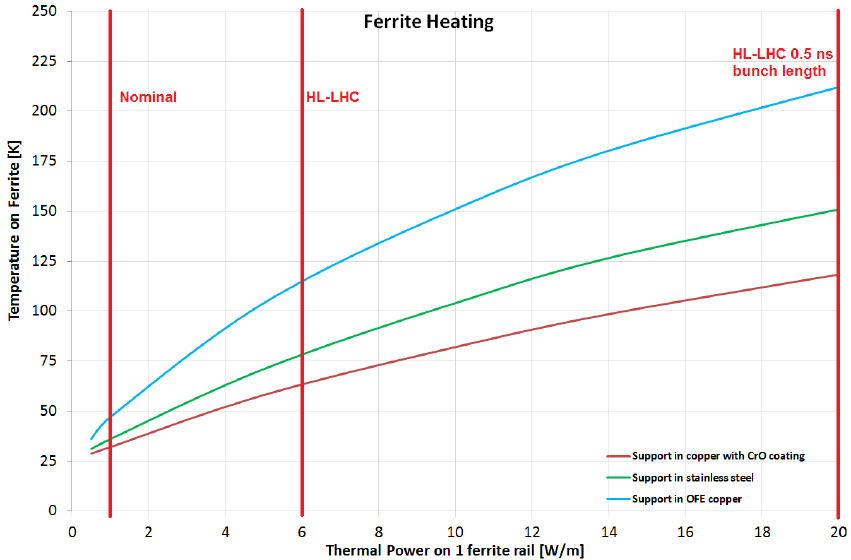
\includegraphics[width=0.75\textwidth]{LHC_Collimation_Upgrades/figures/temp_increase_tctp_col.png}
\end{center}
\label{fig:tctp-ferrite-temp-rise}
\caption{The temperature increase of the ferrite damping tiles in the TCTP collimator under a number of beam operating conditions and for a number of different jaw support materials. Plot taken from [cite Carra and Garlasche].}
\end{figure}

%%%%%% LHC Injection Kicker Magnet %%%%%%

\chapter{LHC Injection Kicker Magnet}

\begin{itemize}
\item{Introduction to the kicker magnet system}
\begin{enumerate}
\item{What are kicker magnets - Injection/Extractions systems}
\item{Why are they potentially a problem}
\end{enumerate}
\item{Explain the background of the LHC-MKI in particular}
\begin{enumerate}
\item{The original concern over heating, subsequent design of the beam screen}
\item{Observed problems with electrical breakdown of the beam screen, and subsequent removal of screen conductors}
\item{Recent observed heating in MKIs}
\end{enumerate}
\item{Summarise current state of the MKIs in the LHC - Beam screen layouts, two sets of kickers, one all of 15 screen conductors, one has one with 24}
\end{itemize}
\input{LHC_MKI/observations_during_operation}

\section{LHC Injection Kicker Magnet}

\begin{itemize}
\item{Introduction to the kicker magnet system}
\begin{enumerate}
\item{What are kicker magnets - Injection/Extractions systems}
\item{Why are they potentially a problem}
\end{enumerate}
\item{Explain the background of the LHC-MKI in particular}
\begin{enumerate}
\item{The original concern over heating, subsequent design of the beam screen}
\item{Observed problems with electrical breakdown of the beam screen, and subsequent removal of screen conductors}
\item{Recent observed heating in MKIs}
\end{enumerate}
\item{Summarise current state of the MKIs in the LHC - Beam screen layouts, two sets of kickers, one all of 15 screen conductors, one has one with 24}
\item{Comparison of the measurements and simulations of the LHC-MKI}
\begin{enumerate}
\item{Measurements of the Longitudinal BCI of the MKI - before and after bake out, with 15 and 19 screen conductors}
\item{Measurements of the transverse BCI of the MKI - if time just for interest and as a verification of the asymmetric method}
\end{enumerate}
\item{A breakdown of the impedance that we see in the MKI}
\begin{enumerate}
\item{Start with a simple c - core ferrite magnet}
\item{Add a ceramic tube}
\item{Add screen conductors in internal side - Brief interlude about the limitations this places on the magnet rise time due to creating a Faraday cage}
\item{Add the capacitive coupling - Different lengths of overlap to demonstrate that this controls the frequency of the resonances. Also lengths of the screen conductors for lower resonances}
\item{Add the ferrite damping rings - damp resonances of length of screen conductor - not(!) overlap}
\item{Hopefully show that this is the dominant cause of the resonances}
\end{enumerate}
\item{Summary of different beam screen designs - Where possible include discussion about the reduction of the voltage build up on each screen conductor}
\begin{enumerate}
\item{Screen conductors all of the same length with capactive coupling at one end - Show how increasing the number of screen conductors really helps to reduce the BCI}
\item{Screen conductors with a tapering of the length, with the longest at the side towards the ground plate and the shortest towards the HV plate}
\item{Alternating lengths of long and short screen conductors}
\item{Having the screen conductors in closed slots in the ceramic tube}
\item{The addition of small conducting spheres to the ends of the screen conductors to reduce the high fields at the conductor ends}
\item{Thicker ceramic at the capacitively coupled end of the beam screen to reduce the field gradient}
\item{Alternative beam screen design - Most screen conductor capactively coupled at both ends, with two connected to the beam pipe at one end. Aim to reduce the potential on all conductors by conductively connecting them at the capactively coupled end}
\item{Stepping the external metallization away from the ceramic tube at the ends of the screen conductors. The metallization will be removed and a conducting pipe placed there instead - different step out dstances are investigated}
\end{enumerate}

\item{Heating estimates for all of the above}
\begin{enumerate}
\item{Explain completely the methods of estimating the power losses here - bunch intensity, number of bunches, bunch length, distribution}
\item{Note the benefits of increasing the bunch length for the resonances with 15 screen conductors}
\item{Summary charts of the beam induced heating for the others, and plots illustrating how the changes in bunch length changes the power loss}
\item{Impedance profiles of all of the above - longitudinal predominantly}
\item{Some judgement on which is most appropriate for an impedance point of view}
\item{Comments on the improvements made to existing magnets already - 19 screen conductors}
\end{enumerate}
\end{itemize}
%
% Introduction to kicker magnet systems - PFNs and the materials normally used
% Risks of beam coupling impedance to the kicker magnet system
% Existing beam coupling impedance reduction - ceramic screen with conductive inserts. Limits of this (electrical breakdown)
% First - comparison of simulations to measurements
% Second - Proposals of improvements to the reduction measures - Rounded ends, changing strips arrangements
% Evaluation of new proposals - comparison of heat load (different methods of evaluating heat load (assume crosses resonance, or real spectrum)), explaination of 
% spectrum measurements and the differences bunch length and profile can make
%
%
%



\section{LHC Phase 2 Collimator Designs}
\begin{itemize}
\item{Introduction to the collimator upgrade project - Why are collimators important}
\begin{enumerate}
\item{The have two significant physical requirements - a rigid, sturdy material and must be placed very close to the beam}
\item{The first necessitated the use of graphite/carbon materials for the phase 1 collimators due to their survivability in the condition needed. The second means that the resistive wall impedance is very large}
\end{enumerate}
\item{Phase 2 collimator materials choice}
\begin{enumerate}
\item{Why a phase 2 collimator upgrade?}
\item{Summary of the material requirements and the available materials}
\item{Simple model used - simulations and comparison to analytical models}
\end{enumerate}
\item{TCTP Impedance Studies}
\begin{enumerate}
\item{What is the TCTP? Why do we need it?}
\item{Possibly designs}
\begin{itemize}
\item{Structure with RF fingers isolating the beam from the vacuum tank}
\item{Structure with a narrow connection between central cavity and vacuum tank - simulated with and without ferrite to demonstrate reduction in Q}
\end{itemize}
\item{Simulations Parameters and results}
\item{Heating estimates - using single bunch, multi-bunch, on resonance and equally spaced}
\item{Localisation of the heating - using both CST and HFSS}

\end{enumerate}
\end{itemize}
%
% Introduction to the new collimator design - Old collimator design, problems with sliding rails, new design, new material possibilities
% Material Evaluation - Comparison of CST simulations
% Whole collimator simulations of phase 2 secondary - Transverse and longitudinal modes with ferrite - compared to that from phase 1
% Sims in CST PS, GdFidl and HFSS
% Heating calculations also
%
%
%
%
%



\begin{enumerate}
\item{Start with a simple c - core ferrite magnet}
\item{Add a ceramic tube}
\item{Add screen conductors in internal side - Brief interlude about the limitations this places on the magnet rise time due to creating a Faraday cage}
\item{Add the capacitive coupling - Different lengths of overlap to demonstrate that this controls the frequency of the resonances. Also lengths of the screen conductors for lower resonances}
\item{Add the ferrite damping rings - damp resonances of length of screen conductor - not(!) overlap}
\item{Hopefully show that this is the dominant cause of the resonances}
\end{enumerate}


\section{LHC Injection Kicker Magnet}

\begin{itemize}
\item{Introduction to the kicker magnet system}
\begin{enumerate}
\item{What are kicker magnets - Injection/Extractions systems}
\item{Why are they potentially a problem}
\end{enumerate}
\item{Explain the background of the LHC-MKI in particular}
\begin{enumerate}
\item{The original concern over heating, subsequent design of the beam screen}
\item{Observed problems with electrical breakdown of the beam screen, and subsequent removal of screen conductors}
\item{Recent observed heating in MKIs}
\end{enumerate}
\item{Summarise current state of the MKIs in the LHC - Beam screen layouts, two sets of kickers, one all of 15 screen conductors, one has one with 24}
\item{Comparison of the measurements and simulations of the LHC-MKI}
\begin{enumerate}
\item{Measurements of the Longitudinal BCI of the MKI - before and after bake out, with 15 and 19 screen conductors}
\item{Measurements of the transverse BCI of the MKI - if time just for interest and as a verification of the asymmetric method}
\end{enumerate}
\item{A breakdown of the impedance that we see in the MKI}
\begin{enumerate}
\item{Start with a simple c - core ferrite magnet}
\item{Add a ceramic tube}
\item{Add screen conductors in internal side - Brief interlude about the limitations this places on the magnet rise time due to creating a Faraday cage}
\item{Add the capacitive coupling - Different lengths of overlap to demonstrate that this controls the frequency of the resonances. Also lengths of the screen conductors for lower resonances}
\item{Add the ferrite damping rings - damp resonances of length of screen conductor - not(!) overlap}
\item{Hopefully show that this is the dominant cause of the resonances}
\end{enumerate}
\item{Summary of different beam screen designs - Where possible include discussion about the reduction of the voltage build up on each screen conductor}
\begin{enumerate}
\item{Screen conductors all of the same length with capactive coupling at one end - Show how increasing the number of screen conductors really helps to reduce the BCI}
\item{Screen conductors with a tapering of the length, with the longest at the side towards the ground plate and the shortest towards the HV plate}
\item{Alternating lengths of long and short screen conductors}
\item{Having the screen conductors in closed slots in the ceramic tube}
\item{The addition of small conducting spheres to the ends of the screen conductors to reduce the high fields at the conductor ends}
\item{Thicker ceramic at the capacitively coupled end of the beam screen to reduce the field gradient}
\item{Alternative beam screen design - Most screen conductor capactively coupled at both ends, with two connected to the beam pipe at one end. Aim to reduce the potential on all conductors by conductively connecting them at the capactively coupled end}
\item{Stepping the external metallization away from the ceramic tube at the ends of the screen conductors. The metallization will be removed and a conducting pipe placed there instead - different step out dstances are investigated}
\end{enumerate}

\item{Heating estimates for all of the above}
\begin{enumerate}
\item{Explain completely the methods of estimating the power losses here - bunch intensity, number of bunches, bunch length, distribution}
\item{Note the benefits of increasing the bunch length for the resonances with 15 screen conductors}
\item{Summary charts of the beam induced heating for the others, and plots illustrating how the changes in bunch length changes the power loss}
\item{Impedance profiles of all of the above - longitudinal predominantly}
\item{Some judgement on which is most appropriate for an impedance point of view}
\item{Comments on the improvements made to existing magnets already - 19 screen conductors}
\end{enumerate}
\end{itemize}
%
% Introduction to kicker magnet systems - PFNs and the materials normally used
% Risks of beam coupling impedance to the kicker magnet system
% Existing beam coupling impedance reduction - ceramic screen with conductive inserts. Limits of this (electrical breakdown)
% First - comparison of simulations to measurements
% Second - Proposals of improvements to the reduction measures - Rounded ends, changing strips arrangements
% Evaluation of new proposals - comparison of heat load (different methods of evaluating heat load (assume crosses resonance, or real spectrum)), explaination of 
% spectrum measurements and the differences bunch length and profile can make
%
%
%



%
% Introduction to the new collimator design - Old collimator design, problems with sliding rails, new design, new material possibilities
% Material Evaluation - Comparison of CST simulations
% Whole collimator simulations of phase 2 secondary - Transverse and longitudinal modes with ferrite - compared to that from phase 1
% Sims in CST PS, GdFidl and HFSS
% Heating calculations also
%
%
%
%
%





\begin{itemize}

\item{Summary of different beam screen designs - Where possible include discussion about the reduction of the voltage build up on each screen conductor}
\begin{enumerate}
\item{Screen conductors all of the same length with capactive coupling at one end - Show how increasing the number of screen conductors really helps to reduce the BCI}
\item{Screen conductors with a tapering of the length, with the longest at the side towards the ground plate and the shortest towards the HV plate}
\item{Alternating lengths of long and short screen conductors}
\item{Having the screen conductors in closed slots in the ceramic tube}
\item{The addition of small conducting spheres to the ends of the screen conductors to reduce the high fields at the conductor ends}
\item{Thicker ceramic at the capacitively coupled end of the beam screen to reduce the field gradient}
\item{Alternative beam screen design - Most screen conductor capactively coupled at both ends, with two connected to the beam pipe at one end. Aim to reduce the potential on all conductors by conductively connecting them at the capactively coupled end}
\item{Stepping the external metallization away from the ceramic tube at the ends of the screen conductors. The metallization will be removed and a conducting pipe placed there instead - different step out dstances are investigated}
\end{enumerate}

\item{Heating estimates for all of the above}
\begin{enumerate}
\item{Explain completely the methods of estimating the power losses here - bunch intensity, number of bunches, bunch length, distribution}
\item{Note the benefits of increasing the bunch length for the resonances with 15 screen conductors}
\item{Summary charts of the beam induced heating for the others, and plots illustrating how the changes in bunch length changes the power loss}
\item{Impedance profiles of all of the above - longitudinal predominantly}
\item{Some judgement on which is most appropriate for an impedance point of view}
\item{Comments on the improvements made to existing magnets already - 19 screen conductors}
\end{enumerate}
\end{itemize}


\section{LHC Injection Kicker Magnet}

\begin{itemize}
\item{Introduction to the kicker magnet system}
\begin{enumerate}
\item{What are kicker magnets - Injection/Extractions systems}
\item{Why are they potentially a problem}
\end{enumerate}
\item{Explain the background of the LHC-MKI in particular}
\begin{enumerate}
\item{The original concern over heating, subsequent design of the beam screen}
\item{Observed problems with electrical breakdown of the beam screen, and subsequent removal of screen conductors}
\item{Recent observed heating in MKIs}
\end{enumerate}
\item{Summarise current state of the MKIs in the LHC - Beam screen layouts, two sets of kickers, one all of 15 screen conductors, one has one with 24}
\item{Comparison of the measurements and simulations of the LHC-MKI}
\begin{enumerate}
\item{Measurements of the Longitudinal BCI of the MKI - before and after bake out, with 15 and 19 screen conductors}
\item{Measurements of the transverse BCI of the MKI - if time just for interest and as a verification of the asymmetric method}
\end{enumerate}
\item{A breakdown of the impedance that we see in the MKI}
\begin{enumerate}
\item{Start with a simple c - core ferrite magnet}
\item{Add a ceramic tube}
\item{Add screen conductors in internal side - Brief interlude about the limitations this places on the magnet rise time due to creating a Faraday cage}
\item{Add the capacitive coupling - Different lengths of overlap to demonstrate that this controls the frequency of the resonances. Also lengths of the screen conductors for lower resonances}
\item{Add the ferrite damping rings - damp resonances of length of screen conductor - not(!) overlap}
\item{Hopefully show that this is the dominant cause of the resonances}
\end{enumerate}
\item{Summary of different beam screen designs - Where possible include discussion about the reduction of the voltage build up on each screen conductor}
\begin{enumerate}
\item{Screen conductors all of the same length with capactive coupling at one end - Show how increasing the number of screen conductors really helps to reduce the BCI}
\item{Screen conductors with a tapering of the length, with the longest at the side towards the ground plate and the shortest towards the HV plate}
\item{Alternating lengths of long and short screen conductors}
\item{Having the screen conductors in closed slots in the ceramic tube}
\item{The addition of small conducting spheres to the ends of the screen conductors to reduce the high fields at the conductor ends}
\item{Thicker ceramic at the capacitively coupled end of the beam screen to reduce the field gradient}
\item{Alternative beam screen design - Most screen conductor capactively coupled at both ends, with two connected to the beam pipe at one end. Aim to reduce the potential on all conductors by conductively connecting them at the capactively coupled end}
\item{Stepping the external metallization away from the ceramic tube at the ends of the screen conductors. The metallization will be removed and a conducting pipe placed there instead - different step out dstances are investigated}
\end{enumerate}

\item{Heating estimates for all of the above}
\begin{enumerate}
\item{Explain completely the methods of estimating the power losses here - bunch intensity, number of bunches, bunch length, distribution}
\item{Note the benefits of increasing the bunch length for the resonances with 15 screen conductors}
\item{Summary charts of the beam induced heating for the others, and plots illustrating how the changes in bunch length changes the power loss}
\item{Impedance profiles of all of the above - longitudinal predominantly}
\item{Some judgement on which is most appropriate for an impedance point of view}
\item{Comments on the improvements made to existing magnets already - 19 screen conductors}
\end{enumerate}
\end{itemize}
%
% Introduction to kicker magnet systems - PFNs and the materials normally used
% Risks of beam coupling impedance to the kicker magnet system
% Existing beam coupling impedance reduction - ceramic screen with conductive inserts. Limits of this (electrical breakdown)
% First - comparison of simulations to measurements
% Second - Proposals of improvements to the reduction measures - Rounded ends, changing strips arrangements
% Evaluation of new proposals - comparison of heat load (different methods of evaluating heat load (assume crosses resonance, or real spectrum)), explaination of 
% spectrum measurements and the differences bunch length and profile can make
%
%
%



\section{LHC Phase 2 Collimator Designs}
\begin{itemize}
\item{Introduction to the collimator upgrade project - Why are collimators important}
\begin{enumerate}
\item{The have two significant physical requirements - a rigid, sturdy material and must be placed very close to the beam}
\item{The first necessitated the use of graphite/carbon materials for the phase 1 collimators due to their survivability in the condition needed. The second means that the resistive wall impedance is very large}
\end{enumerate}
\item{Phase 2 collimator materials choice}
\begin{enumerate}
\item{Why a phase 2 collimator upgrade?}
\item{Summary of the material requirements and the available materials}
\item{Simple model used - simulations and comparison to analytical models}
\end{enumerate}
\item{TCTP Impedance Studies}
\begin{enumerate}
\item{What is the TCTP? Why do we need it?}
\item{Possibly designs}
\begin{itemize}
\item{Structure with RF fingers isolating the beam from the vacuum tank}
\item{Structure with a narrow connection between central cavity and vacuum tank - simulated with and without ferrite to demonstrate reduction in Q}
\end{itemize}
\item{Simulations Parameters and results}
\item{Heating estimates - using single bunch, multi-bunch, on resonance and equally spaced}
\item{Localisation of the heating - using both CST and HFSS}

\end{enumerate}
\end{itemize}
%
% Introduction to the new collimator design - Old collimator design, problems with sliding rails, new design, new material possibilities
% Material Evaluation - Comparison of CST simulations
% Whole collimator simulations of phase 2 secondary - Transverse and longitudinal modes with ferrite - compared to that from phase 1
% Sims in CST PS, GdFidl and HFSS
% Heating calculations also
%
%
%
%
%




\section{LHC Injection Kicker Magnet}

\begin{itemize}
\item{Introduction to the kicker magnet system}
\begin{enumerate}
\item{What are kicker magnets - Injection/Extractions systems}
\item{Why are they potentially a problem}
\end{enumerate}
\item{Explain the background of the LHC-MKI in particular}
\begin{enumerate}
\item{The original concern over heating, subsequent design of the beam screen}
\item{Observed problems with electrical breakdown of the beam screen, and subsequent removal of screen conductors}
\item{Recent observed heating in MKIs}
\end{enumerate}
\item{Summarise current state of the MKIs in the LHC - Beam screen layouts, two sets of kickers, one all of 15 screen conductors, one has one with 24}
\item{Comparison of the measurements and simulations of the LHC-MKI}
\begin{enumerate}
\item{Measurements of the Longitudinal BCI of the MKI - before and after bake out, with 15 and 19 screen conductors}
\item{Measurements of the transverse BCI of the MKI - if time just for interest and as a verification of the asymmetric method}
\end{enumerate}
\item{A breakdown of the impedance that we see in the MKI}
\begin{enumerate}
\item{Start with a simple c - core ferrite magnet}
\item{Add a ceramic tube}
\item{Add screen conductors in internal side - Brief interlude about the limitations this places on the magnet rise time due to creating a Faraday cage}
\item{Add the capacitive coupling - Different lengths of overlap to demonstrate that this controls the frequency of the resonances. Also lengths of the screen conductors for lower resonances}
\item{Add the ferrite damping rings - damp resonances of length of screen conductor - not(!) overlap}
\item{Hopefully show that this is the dominant cause of the resonances}
\end{enumerate}
\item{Summary of different beam screen designs - Where possible include discussion about the reduction of the voltage build up on each screen conductor}
\begin{enumerate}
\item{Screen conductors all of the same length with capactive coupling at one end - Show how increasing the number of screen conductors really helps to reduce the BCI}
\item{Screen conductors with a tapering of the length, with the longest at the side towards the ground plate and the shortest towards the HV plate}
\item{Alternating lengths of long and short screen conductors}
\item{Having the screen conductors in closed slots in the ceramic tube}
\item{The addition of small conducting spheres to the ends of the screen conductors to reduce the high fields at the conductor ends}
\item{Thicker ceramic at the capacitively coupled end of the beam screen to reduce the field gradient}
\item{Alternative beam screen design - Most screen conductor capactively coupled at both ends, with two connected to the beam pipe at one end. Aim to reduce the potential on all conductors by conductively connecting them at the capactively coupled end}
\item{Stepping the external metallization away from the ceramic tube at the ends of the screen conductors. The metallization will be removed and a conducting pipe placed there instead - different step out dstances are investigated}
\end{enumerate}

\item{Heating estimates for all of the above}
\begin{enumerate}
\item{Explain completely the methods of estimating the power losses here - bunch intensity, number of bunches, bunch length, distribution}
\item{Note the benefits of increasing the bunch length for the resonances with 15 screen conductors}
\item{Summary charts of the beam induced heating for the others, and plots illustrating how the changes in bunch length changes the power loss}
\item{Impedance profiles of all of the above - longitudinal predominantly}
\item{Some judgement on which is most appropriate for an impedance point of view}
\item{Comments on the improvements made to existing magnets already - 19 screen conductors}
\end{enumerate}
\end{itemize}
%
% Introduction to kicker magnet systems - PFNs and the materials normally used
% Risks of beam coupling impedance to the kicker magnet system
% Existing beam coupling impedance reduction - ceramic screen with conductive inserts. Limits of this (electrical breakdown)
% First - comparison of simulations to measurements
% Second - Proposals of improvements to the reduction measures - Rounded ends, changing strips arrangements
% Evaluation of new proposals - comparison of heat load (different methods of evaluating heat load (assume crosses resonance, or real spectrum)), explaination of 
% spectrum measurements and the differences bunch length and profile can make
%
%
%



\section{LHC Phase 2 Collimator Designs}
\begin{itemize}
\item{Introduction to the collimator upgrade project - Why are collimators important}
\begin{enumerate}
\item{The have two significant physical requirements - a rigid, sturdy material and must be placed very close to the beam}
\item{The first necessitated the use of graphite/carbon materials for the phase 1 collimators due to their survivability in the condition needed. The second means that the resistive wall impedance is very large}
\end{enumerate}
\item{Phase 2 collimator materials choice}
\begin{enumerate}
\item{Why a phase 2 collimator upgrade?}
\item{Summary of the material requirements and the available materials}
\item{Simple model used - simulations and comparison to analytical models}
\end{enumerate}
\item{TCTP Impedance Studies}
\begin{enumerate}
\item{What is the TCTP? Why do we need it?}
\item{Possibly designs}
\begin{itemize}
\item{Structure with RF fingers isolating the beam from the vacuum tank}
\item{Structure with a narrow connection between central cavity and vacuum tank - simulated with and without ferrite to demonstrate reduction in Q}
\end{itemize}
\item{Simulations Parameters and results}
\item{Heating estimates - using single bunch, multi-bunch, on resonance and equally spaced}
\item{Localisation of the heating - using both CST and HFSS}

\end{enumerate}
\end{itemize}
%
% Introduction to the new collimator design - Old collimator design, problems with sliding rails, new design, new material possibilities
% Material Evaluation - Comparison of CST simulations
% Whole collimator simulations of phase 2 secondary - Transverse and longitudinal modes with ferrite - compared to that from phase 1
% Sims in CST PS, GdFidl and HFSS
% Heating calculations also
%
%
%
%
%





\chapter{Conclusions}

\bibliographystyle{IEEEtran}
\bibliography{general_bibliography}

\end{document}
